\documentclass[graybox, envcountchap]{svmult}
% Springer document settings
\usepackage[bottom]{footmisc}% places footnotes at page bottom

\usepackage{newtxtext}       % 
\usepackage[varvw]{newtxmath}       % selects Times Roman as basic font
%%%%%%%%%%%%%%%%%%%%%%%%%%%%%%%

% \usepackage{amssymb}
\usepackage{ntheorem}
\usepackage{amsmath}
\usepackage{enumitem}


\usepackage{graphicx}
\usepackage{color}
\usepackage{cite}
\usepackage{makeidx}


\usepackage{ascmac}
\usepackage{eclbkbox}
\usepackage{dsfont}

\usepackage{longtable}

\usepackage{url}

\usepackage{hyperref}

\usepackage{multicol}

%% --川口追加--
\makeatletter
\let\MYcaption\@makecaption
\makeatother
\usepackage{subcaption}
\captionsetup{compatibility=false}      % 必要に応じて

\makeatletter
\let\@makecaption\MYcaption
\makeatother
% ----

%%
\theoremstyle{plain}
\theoremheaderfont{\bfseries}
\theorembodyfont{\rmfamily}
\theoremseparator{\hspace{1ex}}
\theoremindent0cm
\theoremnumbering{arabic}
\theoremprework{\vspace{1ex}\begin{shadebox}\vspace{1ex}}
\theorempostwork{\vspace{-1ex}\end{shadebox}\vspace{1ex}}

%%
\theoremclass{theorem}

%%
\theoremclass{theorem}

%%
\theoremclass{theorem}


%%
\theoremstyle{break}
\theoremheaderfont{\bfseries}
\theorembodyfont{\rmfamily}
\theoremseparator{}
\theoremindent0cm
\theoremnumbering{arabic}
\theoremprework{\vspace{1.5ex}\begin{breakbox}\vspace{-0.5ex}}
\theorempostwork{\vspace{-0.5ex}\end{breakbox}\vspace{1.5ex}}

%%
\theoremstyle{nonumberplain}
\theoremseparator{\hspace{1ex}}

%%
\newtheorem{assumption}{Assumption}[section]

%%
\renewcommand{\theproblem}{}

\renewcommand{\theremark}{}


\newcommand{\red}[1]{{\color{red}#1}}
\newcommand{\blue}[1]{{\color{blue}#1}}
\newcommand{\green}[1]{{\color{green}#1}}

\DeclareMathOperator*{\argmax}{arg\,max}

\newcommand{\bm}[1]{\boldsymbol{#1}}
\newcommand{\sfT}{\mathsf{T}}

\newcommand{\advanced}{$^{\ddag}$}

\DeclareMathOperator{\sfsin}{\mathsf{sin}}
\DeclareMathOperator{\sfcos}{\mathsf{cos}}
\DeclareMathOperator{\sftan}{\mathsf{tan}}
\DeclareMathOperator{\sfarctan}{\mathsf{arctan}}

\DeclareMathOperator{\sfdiag}{\mathsf{diag}}
\DeclareMathOperator{\sfcol}{\mathsf{col}}
\DeclareMathOperator{\sfdet}{\mathsf{det}}
\DeclareMathOperator{\sfadj}{\mathsf{adj}}
\DeclareMathOperator{\sftrace}{\mathsf{trace}}

\DeclareMathOperator{\real}{\mathsf{Re}}

\DeclareMathOperator{\sfker}{\mathsf{ker}}
\DeclareMathOperator{\sfim}{\mathsf{im}}

\DeclareMathOperator{\sfdim}{\mathsf{dim}}
\DeclareMathOperator{\sfspan}{\mathsf{span}}

\DeclareMathOperator{\sfint}{\mathsf{int}}

\DeclareMathOperator*{\sfmin}{\mathsf{min}}
\DeclareMathOperator*{\sfmax}{\mathsf{max}}
\DeclareMathOperator*{\sfsup}{\mathsf{sup}}

\DeclareMathOperator{\sfsat}{\mathsf{sat}}

\newcommand{\mat}[1]{\left[\: \begin{matrix} #1 \end{matrix} \:\right]}
\newcommand{\spliteq}[1]{\begin{split} #1 \end{split}}
\newcommand{\simode}[1]{\begin{cases}  \begin{split} #1 \end{split} \end{cases}}

\newcommand{\proofend}{\hfill \rule{2mm}{3mm}}

\newcommand{\Xti}{X_i'}
\newcommand{\Xsi}{X_i}

\newcommand{\Xtone}{X_1'}
\newcommand{\XtN}{X_N'}

\newcommand{\Xt}{X'}
\newcommand{\Xs}{X}

\newcommand{\taudi}{\tau_i}
\newcommand{\taud}{\tau}

\newcommand{\Cgi}{b_i}


\newcommand{\Ifd}{I_{\rm field} }

\newcommand{\matlab}{\textsc{Matlab} }





%% --川口追加--
\newcommand{\thshift}{\theta_{12}}
\newcommand{\thshiftb}{\theta_{32}}
\newcommand{\Ysa}{\bm y_{12}}
\newcommand{\bca}{c_{12}}
\newcommand{\Ysb}{\bm y_{32}}
\newcommand{\bcb}{c_{32}}
\newcommand{\bcij}{c_{ij}}
\newcommand{\Is}{{\bm I}_{12}' }
\newcommand{\im}{\bm j}
\newcommand{\tr}{{\sf T}}

%%%%%%%%%%%%%%%%%%%%%%%%% code lines %%%%%%%%%%%%%%%%%%%%%%%%%%%%%%%%%%%%%%%%%%
\usepackage{listings}
\usepackage{xcolor}
\renewcommand{\lstlistingname}{Program}% Listing -> Algorithm
\renewcommand{\lstlistlistingname}{List of \lstlistingname s}% List of Listings -> List of Algorithms

\definecolor{codegreen}{rgb}{0,0.6,0}
\definecolor{codegray}{rgb}{0.5,0.5,0.5}
\definecolor{codepurple}{rgb}{0.58,0,0.82}
\definecolor{backcolour}{rgb}{0.95,0.95,0.92}

\lstdefinestyle{mystyle}{
    backgroundcolor=\color{backcolour},   
    commentstyle=\color{codegreen},
    keywordstyle=\color{magenta},
    numberstyle=\tiny\color{codegray},
    stringstyle=\color{codepurple},
    basicstyle=\ttfamily\footnotesize,
    breakatwhitespace=false,         
    breaklines=true,                 
    captionpos=b,                    
    keepspaces=true,                 
    numbers=left,                    
    numbersep=5pt,                  
    showspaces=false,                
    showstringspaces=false,
    showtabs=false,                  
    tabsize=2
}

\lstset{style=mystyle}


% Springer document settings
\usepackage[bottom]{footmisc}% places footnotes at page bottom

\usepackage{newtxtext}       % 
\usepackage[varvw]{newtxmath}       % selects Times Roman as basic font
%%%%%%%%%%%%%%%%%%%%%%%%%%%%%%%

% \usepackage{amssymb}
\usepackage{ntheorem}
\usepackage{amsmath}
\usepackage{enumitem}


\usepackage{graphicx}
\usepackage{color}
\usepackage{cite}
\usepackage{makeidx}


\usepackage{ascmac}
\usepackage{eclbkbox}
\usepackage{dsfont}

\usepackage{longtable}

\usepackage{url}

\usepackage{hyperref}

\usepackage{multicol}

%% --川口追加--
\makeatletter
\let\MYcaption\@makecaption
\makeatother
\usepackage{subcaption}
\captionsetup{compatibility=false}      % 必要に応じて

\makeatletter
\let\@makecaption\MYcaption
\makeatother
% ----

%%
\theoremstyle{plain}
\theoremheaderfont{\bfseries}
\theorembodyfont{\rmfamily}
\theoremseparator{\hspace{1ex}}
\theoremindent0cm
\theoremnumbering{arabic}
\theoremprework{\vspace{1ex}\begin{shadebox}\vspace{1ex}}
\theorempostwork{\vspace{-1ex}\end{shadebox}\vspace{1ex}}

%%
\theoremclass{theorem}

%%
\theoremclass{theorem}

%%
\theoremclass{theorem}


%%
\theoremstyle{break}
\theoremheaderfont{\bfseries}
\theorembodyfont{\rmfamily}
\theoremseparator{}
\theoremindent0cm
\theoremnumbering{arabic}
\theoremprework{\vspace{1.5ex}\begin{breakbox}\vspace{-0.5ex}}
\theorempostwork{\vspace{-0.5ex}\end{breakbox}\vspace{1.5ex}}

%%
\theoremstyle{nonumberplain}
\theoremseparator{\hspace{1ex}}

%%
\newtheorem{assumption}{Assumption}[section]

%%
\renewcommand{\theproblem}{}

\renewcommand{\theremark}{}


\newcommand{\red}[1]{{\color{red}#1}}
\newcommand{\blue}[1]{{\color{blue}#1}}
\newcommand{\green}[1]{{\color{green}#1}}

\DeclareMathOperator*{\argmax}{arg\,max}

\newcommand{\bm}[1]{\boldsymbol{#1}}
\newcommand{\sfT}{\mathsf{T}}

\newcommand{\advanced}{$^{\ddag}$}

\DeclareMathOperator{\sfsin}{\mathsf{sin}}
\DeclareMathOperator{\sfcos}{\mathsf{cos}}
\DeclareMathOperator{\sftan}{\mathsf{tan}}
\DeclareMathOperator{\sfarctan}{\mathsf{arctan}}

\DeclareMathOperator{\sfdiag}{\mathsf{diag}}
\DeclareMathOperator{\sfcol}{\mathsf{col}}
\DeclareMathOperator{\sfdet}{\mathsf{det}}
\DeclareMathOperator{\sfadj}{\mathsf{adj}}
\DeclareMathOperator{\sftrace}{\mathsf{trace}}

\DeclareMathOperator{\real}{\mathsf{Re}}

\DeclareMathOperator{\sfker}{\mathsf{ker}}
\DeclareMathOperator{\sfim}{\mathsf{im}}

\DeclareMathOperator{\sfdim}{\mathsf{dim}}
\DeclareMathOperator{\sfspan}{\mathsf{span}}

\DeclareMathOperator{\sfint}{\mathsf{int}}

\DeclareMathOperator*{\sfmin}{\mathsf{min}}
\DeclareMathOperator*{\sfmax}{\mathsf{max}}
\DeclareMathOperator*{\sfsup}{\mathsf{sup}}

\DeclareMathOperator{\sfsat}{\mathsf{sat}}

\newcommand{\mat}[1]{\left[\: \begin{matrix} #1 \end{matrix} \:\right]}
\newcommand{\spliteq}[1]{\begin{split} #1 \end{split}}
\newcommand{\simode}[1]{\begin{cases}  \begin{split} #1 \end{split} \end{cases}}

\newcommand{\proofend}{\hfill \rule{2mm}{3mm}}

\newcommand{\Xti}{X_i'}
\newcommand{\Xsi}{X_i}

\newcommand{\Xtone}{X_1'}
\newcommand{\XtN}{X_N'}

\newcommand{\Xt}{X'}
\newcommand{\Xs}{X}

\newcommand{\taudi}{\tau_i}
\newcommand{\taud}{\tau}

\newcommand{\Cgi}{b_i}


\newcommand{\Ifd}{I_{\rm field} }

\newcommand{\matlab}{\textsc{Matlab} }





%% --川口追加--
\newcommand{\thshift}{\theta_{12}}
\newcommand{\thshiftb}{\theta_{32}}
\newcommand{\Ysa}{\bm y_{12}}
\newcommand{\bca}{c_{12}}
\newcommand{\Ysb}{\bm y_{32}}
\newcommand{\bcb}{c_{32}}
\newcommand{\bcij}{c_{ij}}
\newcommand{\Is}{{\bm I}_{12}' }
\newcommand{\im}{\bm j}
\newcommand{\tr}{{\sf T}}

%%%%%%%%%%%%%%%%%%%%%%%%% code lines %%%%%%%%%%%%%%%%%%%%%%%%%%%%%%%%%%%%%%%%%%
\usepackage{listings}
\usepackage{xcolor}
\renewcommand{\lstlistingname}{Program}% Listing -> Algorithm
\renewcommand{\lstlistlistingname}{List of \lstlistingname s}% List of Listings -> List of Algorithms

\definecolor{codegreen}{rgb}{0,0.6,0}
\definecolor{codegray}{rgb}{0.5,0.5,0.5}
\definecolor{codepurple}{rgb}{0.58,0,0.82}
\definecolor{backcolour}{rgb}{0.95,0.95,0.92}

\lstdefinestyle{mystyle}{
    backgroundcolor=\color{backcolour},   
    commentstyle=\color{codegreen},
    keywordstyle=\color{magenta},
    numberstyle=\tiny\color{codegray},
    stringstyle=\color{codepurple},
    basicstyle=\ttfamily\footnotesize,
    breakatwhitespace=false,         
    breaklines=true,                 
    captionpos=b,                    
    keepspaces=true,                 
    numbers=left,                    
    numbersep=5pt,                  
    showspaces=false,                
    showstringspaces=false,
    showtabs=false,                  
    tabsize=2
}

\lstset{style=mystyle}

\begin{document}

\chapter{Stabilization control of an electrical power system model}\label{ch:stabcont}

In this Chapter, we explain the frequency stabilization control and transient stabilization control of the electrical power system model.
This Chapter is structured as follows. First, in Section \ref{sec:agcover}, as a typical example of the frequency stabilization control, we discuss the outline of automatic generation control to control frequency deviations caused by load fluctuations and so on.
In addition, we confirm that the actual steady power flow distribution is changed by adjusting the controller parameters using a numerical simulation.
Next, in Section \ref{sec:mathnpas}, as a developmental topic, we perform a mathematical analysis of the stability related to the frequency stabilization control.
Specifically, we show the relationship of the stable range of the electrical power system model and the convex range of the potential energy function based on the passivity independent of the equilibrium points of a nonlinear system.
Furthermore, in Section \ref{sec:transcont}, we explain the structure and function of a standard auto-voltage adjustor and a system stabilization device used for the transient stabilization control.
Finally, as a developmental topic in Section \ref{sec:retrofit}, we explain the design method of a system stabilization device based on a retrofit control theory.


\section{Frequency stabilization control}\label{sec:agcover}
\subsection{Automatic generation control by a broadcast-type PI controller}\label{sec:broadPI}


\smallskip
\subsubsection{What is automatic generation control?}

In this Section, we explain the operating principle of \textbf{automatic generation control} to appropriately adjust the power generation relative to unknown load fluctuations.
With the automatic generation control, by observing the frequency deviation of several generators, a control operation is performed whereby the power generation is increased if the supply is too low for the electric power demand and decreased if the supply is excessive.

In actual operation of an electrical power system, a central power supply command center performs automatic generation control.
The basic operating principle is common, but there are several methods depending on the purpose.
The goal is to maintain the frequency at around $\pm$ 0.2Hz relative to the standard frequency of 50 Hz or 60 Hz.


A difficulty of the automatic generation control is that there are many unknown constants and variables in an actual electrical power system.
For example, with a time scale of about 30 minutes, total load can be roughly predicted, but changes in individual load cannot be accurately understood.
It is also difficult to accurately know all the constants, such as the impedance of each transmission line.
Therefore, a control algorithm design method that can be applied without knowing the exact model of the entire power system is needed.
In actual power system operation, changes in total demand for a certain area are forecasted using weather forecast information, such as weather and temperature, and past performance information.
Although the size of the area varies depending on the method used, it is impossible to predict demand completely.


On the other hand, as we confirmed with the numerical example of Section \ref{sec:numsimtr}, even in a situation where a supply-demand balance is not achieved, the frequency of generators asymptotically synchronizes.
This fact means that if the external input of one or more generators is appropriately controlled to achieve 0 for their frequency deviation, the frequency deviation of the remaining generators automatically becomes 0.
Specifically, if we calculate the mean frequency deviation of several generators and control the external input of generators so that the mean would be 0, the frequency deviation of all generators can be asymptotically converged at 0.
Such a control operation can be achieved with PI control.


\smallskip
\subsubsection{Formulation of the automatic generation control}

Below, we consider a generator model that uses the voltage phasor of Section \ref{sec:genfund} as the input.
If we discuss the dynamic characteristics again:
\begin{subequations}\label{eq:gendifagc}
\begin{align}
\simode{
\dot{\delta}_i&= \omega_0  \Delta \omega_i \\
M_i   \Delta \dot{\omega}_i&= 
 - D_i \Delta\omega_i  
 - P_i
+P_{{\rm mech}i}
\\
\taudi \dot{E}_i & = 
 -\tfrac{ \Xsi }{ \Xti }E_i
+\left(
\tfrac{ \Xsi }{ \Xti }-1
\right)
|\bm{V}_i| \sfcos (\delta_i - \angle \bm{V}_i ) 
+ V_{{\rm field}i}
}
\end{align}
If active power and reactive power are the output:
\begin{align}\label{eq:PQoutagc}
\spliteq{
P_i &=  \frac{E_i |\bm{V}_i|}{ \Xti } \sfsin (\delta_i - \angle \bm{V}_i), \\
Q_i &=  \frac{E_i|\bm{V}_i|}{ \Xti } \sfcos (\delta_i - \angle \bm{V}_i)
-\frac{|\bm{V}_i|^2}{ \Xti }
}
\end{align}
\end{subequations}
With this expression, we discuss the load model that uses the voltage phasor as the input and the active and reactive power as the output again.
The constant impedance model is:
\begin{subequations}\label{eq:lmodelsagc}
\begin{align}
P_i =  - 
\frac{|\bm{V}_i|^2}{ \real \left[ \overline{\bm{z}}^{\star}_{{\rm load}i} \right] } 
,\qquad
Q_i = - 
\frac{|\bm{V}_i|^2}{ \imag \left[ \overline{\bm{z}}^{\star}_{{\rm load}i} \right] } 
\end{align}
where, $\bm{z}_{{\rm load}i}^{\star}$ is the constant that expresses the impedance of the load.
Similarly, the constant current model is written as a constant $\bm{I}_{{\rm load}i}^{\star}$ that expresses the current phasor of the load:
\begin{align}
P_i = |\bm{V}_i| \real \left[
\bm{I}_{{\rm load}i}^{\star} 
\right],\qquad
Q_i = - |\bm{V}_i| \imag \left[
\bm{I}_{{\rm load}i}^{\star}
\right]
\end{align}
The constant power model uses $P_{{\rm load}i}^{\star}$ and $Q_{{\rm load}i}^{\star} $ as constants:
\begin{align}\label{eq:contpwmod}
P_i=P_{{\rm load}i}^{\star} ,\qquad
 Q_i= Q_{{\rm load}i}^{\star} 
\end{align}
\end{subequations}
As these generator model and load model are combined with algebraic equations: 
\begin{align}\label{eq:PQVgenagc}
\simode{
P_1 + \bm{j} Q_1 &= 
\sum_{j=1}^{N} \overline{\bm{Y}}_{1j} |\bm{V}_1| |\bm{V}_j | e^{\bm{j} (\angle \bm{V}_1 - \angle \bm{V}_j )} \\ 
& \; \;  \vdots \\
P_N + \bm{j} Q_N &= 
\sum_{j=1}^{N} \overline{\bm{Y}}_{Nj} |\bm{V}_N| |\bm{V}_j | e^{\bm{j} (\angle \bm{V}_N - \angle \bm{V}_j )}
}
\end{align}
we can obtain a differential-algebraic equation system model that describes the entire electrical power system.
However, when a subscript set of generator buses is $\mathcal{I}_{\rm G}$ and a subscript set of load bus bars is $\mathcal{I}_{\rm L}$:
\[
\mathcal{I}_{\rm G} :=  \{1,\ldots, n\}
,\qquad
\mathcal{I}_{\rm L} := \{n+1,\ldots, n+m\}
\]
The number of generator buses is $n$ and the number of load bus bars is $m$.
Also, $N$ denotes the total number of busbars $n+m$.

\begin{figure}[t]
\centering
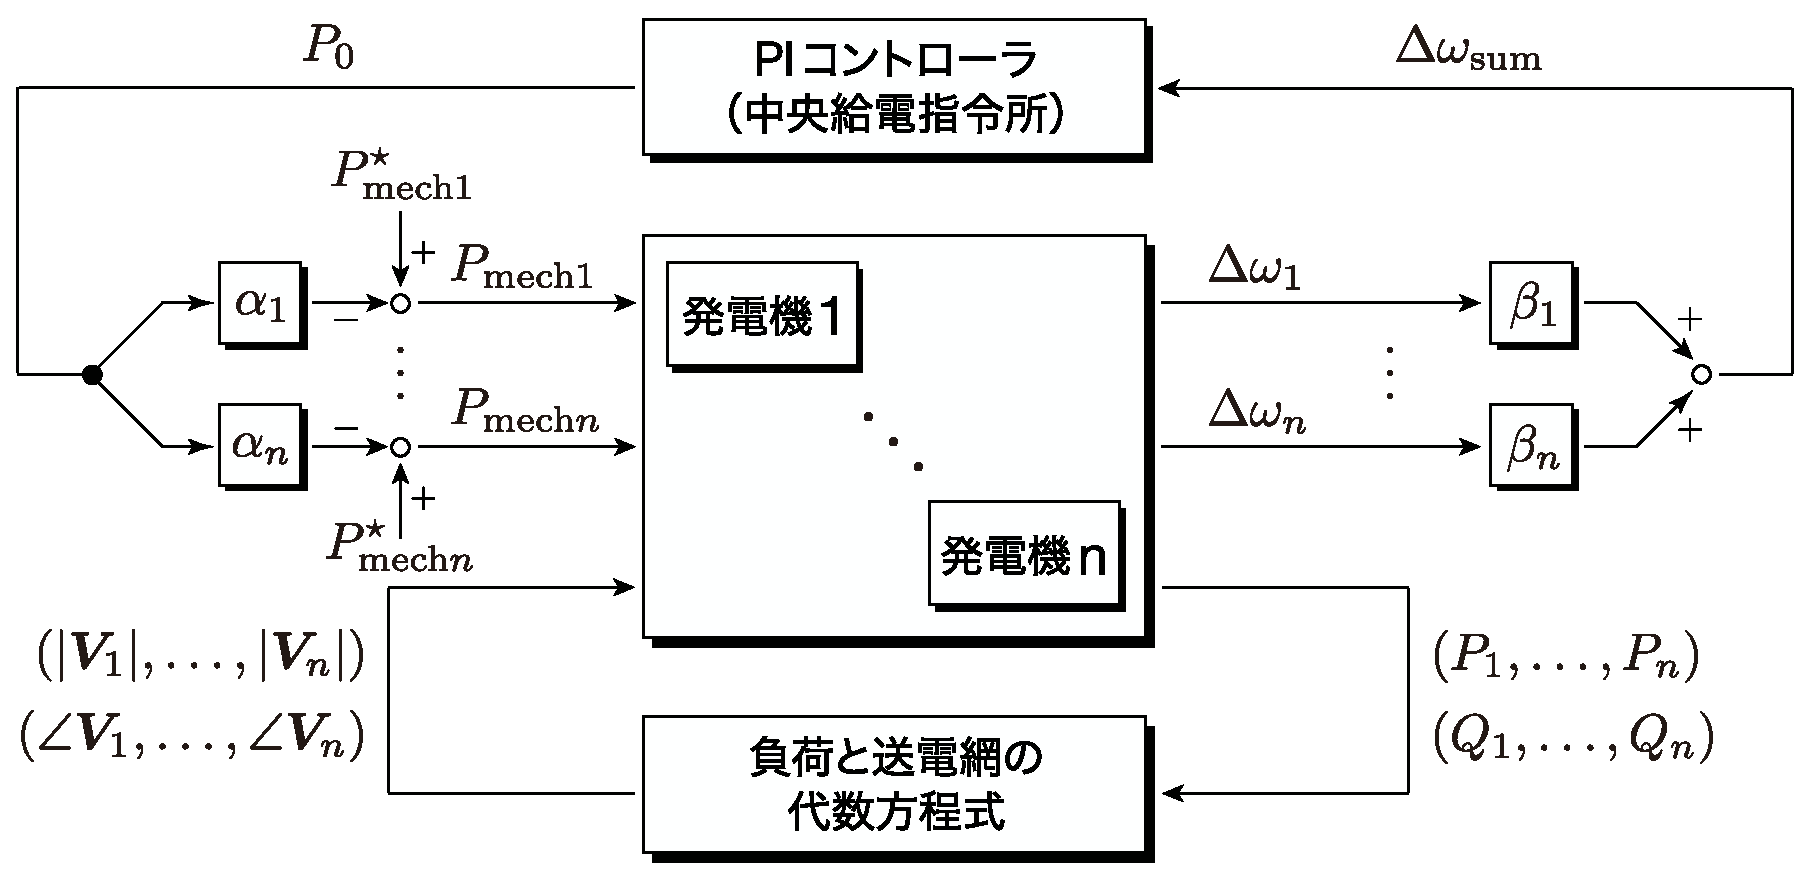
\includegraphics[width = .99\linewidth]{figs/bcAGC}
\medskip
\caption{\textbf{Signal transmission structure for automatic power generation control}}
\label{fig:bcAGC}
\medskip
\end{figure}

The automatic generation control is a control algorithm that adjusts the mechanical torque $P_{{\rm mech}i}$ of Equation (\ref{eq:gendifagc}).
Below, we observe the weighted sum of the frequency deviations related to all generators and consider the broadcast-type PI controller that transmits the control input with an appropriate weight to all generators.
Specifically, for each $i\in \mathcal{I}_{\rm G}$:
\begin{subequations}\label{eq:agccon}
\begin{align}\label{eq:agccona}
P_{{\rm mech}i}(t)=
P_{{\rm mech}i}^{\star} - \alpha_i
\underbrace{
\left\{
k_{\rm P} \Delta \omega_{\rm sum}(t) +
k_{\rm I}
\int_0^t \Delta \omega_{\rm sum}(\tau) d \tau
\right\}
}_{P_{0}(t)}
\end{align}
where $P_{{\rm mech}i}^{\star} $ is a constant that expresses the standard setting of mechanical torque.
$\alpha_i $ is a non-negative constant that specifies the contributions of the generator $i$, and:
\[
\Delta \omega_{\rm sum}(t) := 
\sum_{i =1}^n \beta_i \Delta \omega_{i}(t)
\]
is the weighted sum of the frequency deviation related to the non-negative constant $\beta_i$.
Furthermore, $k_{\rm P}$,$k_{\rm I}$ is a positive definite number that expresses the gain of the PI controller.
This automatic generation contrller has a structure that broadcasts the signals $P_0(t)$ generated by a single PI controller under the weight of $\alpha_i$ and $\beta_i$ to all generators (\FIGref{fig:bcAGC}).
If Equation \ref{eq:agccona} is expressed with differential equations:
\begin{align}
\simode{
\dot{\xi}&=  \Delta \omega_{\rm sum} \\
P_{{\rm mech}i} &= P_{{\rm mech}i}^{\star} - \alpha_i \left(k_{\rm P} \Delta \omega_{\rm sum} +  k_{\rm I} \xi \right)
}
\end{align}
\end{subequations}
With real thermal and nuclear power plants, high-pressure steam generated by the thermal and nuclear power rotates the turbines and generates mechanical torque in a \textbf{prime mover}.
The prime mover has a built-in \textbf{governor} that automatically controls the rotational speed of the generators.
In a more realistic analysis of the automatic generation control, a prime mover model that uses a command from the central power supply command center as the input and the mechanical torque on generators as the output needs to be considered \cite[Chapter 3]{taniguchi2011power}.

By changing the rate of the participation factor, active power supplied by each generator under a steady power flow distribution (wherein supply and demand are balanced) can be adjusted.
From the perspective of control systems engineering, it can be interpreted as “moving a stable equilibrium point of the electrical power system model by switching the controller".
As analyzed in Chapter \ref{sec:staana}, the stability of the electrical power system changes according to the choice of equilibrium points.
In addition, the power generation cost and transmission loss of the entire electrical power system also depend on the way equilibrium points are selected.
Therefore, appropriately switching the participation factor based on the demand distribution improves system stability and lowers the financial cost. 

In the actual operation of an electrical power system, updates to the participation factor are usually made at an interval of several minutes to dozens of minutes \cite[Section 11.1]{kundur1994power}.
With the terminology of electrical power system engineering, the system to update the participation factor is called \textbf{Economic Load Dispatching Control}.
In addition, a control algorithm that uses the participation factor as a constant between the update interval is called \textbf{Load Frequency Control}.
However, attention must be paid since the Economic Load Dispatching Control and Load Frequency Control might not be clearly discriminated, or the Economic Load Dispatching Control might be considered as a different system, depending on the literature. 


\subsection{Numerical simulation of frequency stabilization control}

Using a simple example, let us confirm the effect of frequency stabilization control.

\begin{例}[Stabilization of frequency by the automatic generation control]\label{ex:agcdemo}
Let us consider an electrical power system model consisting of three bus bars discussed in the Example \ref{ex:inires}.
The physical constants of generators and transmission lines are set to the same values as the Example \ref{ex:inires}, and the steady value of \ref{table:genst13b} is set as the initial value of the internal state of generators.
In addition, the field voltage is constant at \ref{table:genst13b}.

Let us consider a 1\% increase in active power consumption from the steady power flow distribution with the initial value from the load of bus bar 2 as the constant power model.
First, the time response of frequency deviation is shown in \FIGref{fig:agcPdemo}(a) when the mechanical torque of the generators is constant at \ref{table:genst13b} and the automatic generation control is not incorporated.
We can see that, as the consumption of electric power increases with the load, supply and demand become unbalanced, and the steady value of the frequency deviation stops being 0.

Next, \FIGref{fig:agcPdemo}(b) shows the result when the broadcast-type PI controller of Equation (\ref{eq:agccon}) is incorporated as the automatic generation control.
The parameters of the controller are set to the values of \ref{table:agcpara}(a).
This Figure shows that, even if the consumed electric power of the load changes due to the effect of the automatic generation control, the frequency deviation is barely generated.
\end{例}


\begin{figure}[t]
  \centering
  {
  \begin{minipage}{0.49\linewidth}
    \centering
    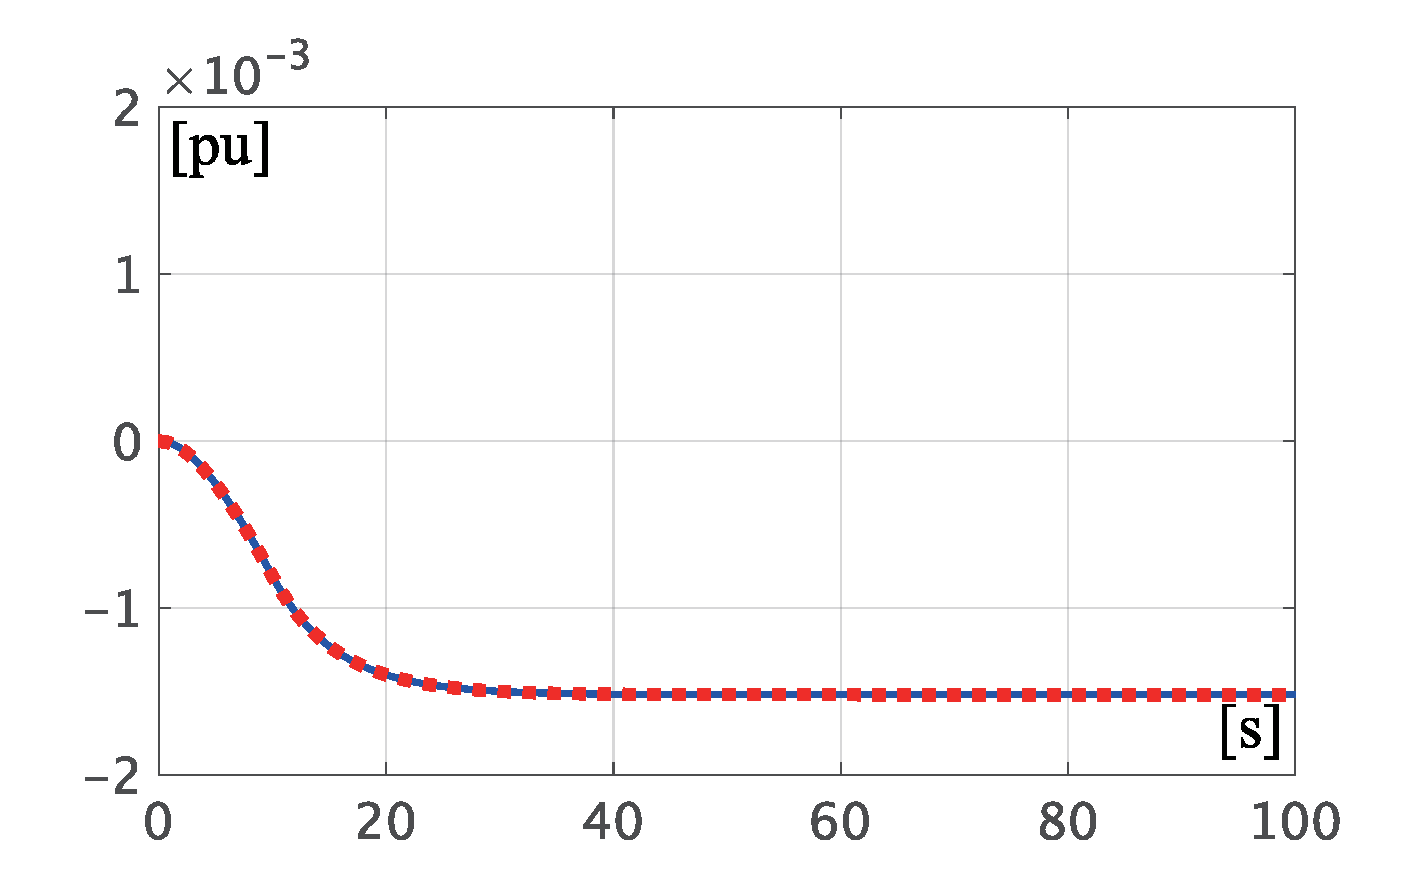
\includegraphics[width = 1.0\linewidth]{figs/woagcPinc}
    \subcaption{No automatic power generation control}
  \end{minipage}
  \begin{minipage}{0.49\linewidth}
    \centering
    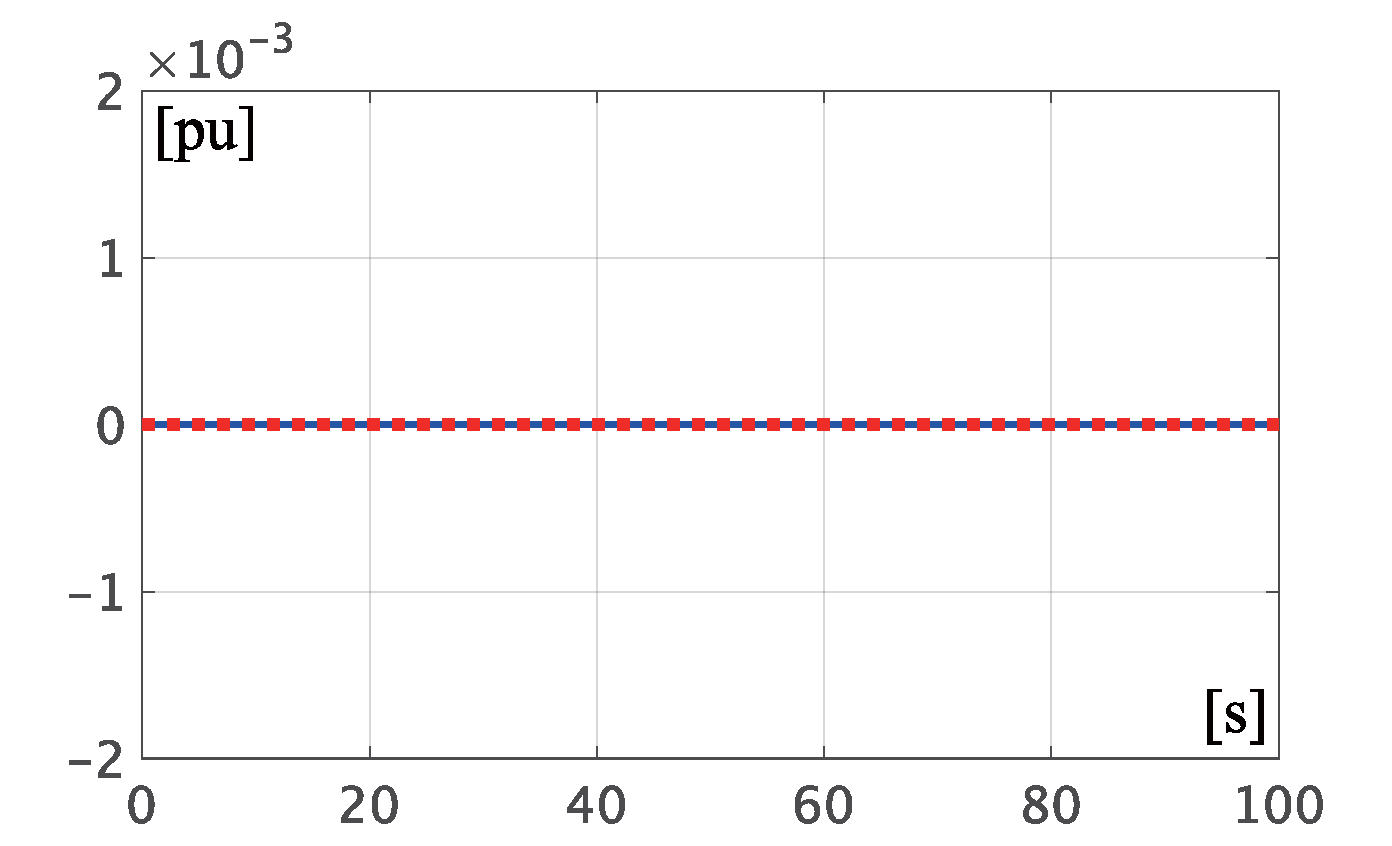
\includegraphics[width = 1.0\linewidth]{figs/wagcPinc}
    \subcaption{With automatic power generation control}
  \end{minipage}
  \medskip
  \caption{\textbf{Time response of angular frequency deviation to power consumption increase} 
    \\ \centering(Blue solid line: $Delta \omega_1$, Red dashed line: $Delta \omega_3$)}
  \label{fig:agcPdemo}
  }
\medskip
\end{figure}

\begin{table}[h]
\medskip
 \caption{\textbf{Controller Parameter Setting}}
 \label{table:agcpara}
 \centering
  \begin{tabular}{ccccccccc}
   \hline
Setup &  $k_{\rm P}$ & $k_{\rm I}$ & $\alpha_1$ & $\alpha_3$ &$\beta_1$ & $\beta_3$ \\
   \hline \hline
(a) & 100 & 500 & 1 & 3 & 1 & 3 \\
(b) & 100 & 500 & 1 & 1& 1 & 1 \\
(c) & 100 & 500 & 3 & 1 & 3 & 1 \\
   \hline
  \end{tabular}
\end{table}

Next, let us confirm that the steady power flow distribution that achieves the supply-demand balance changes by adjusting the participation factor of the broadcast-type PI controller in Equation  (\ref{eq:agccon}).

\begin{例}[Changes in the steady power flow distribution due to adjustment of the participation factor]\label{ex:pfvary}
As in the Example \ref{ex:agcdemo}, let us consider an electrical power system model consisting of two generators and one load.
Here, we confirm that the ratio of active power supplied by generator 1 and generator 3 changes by changing the participation factor of the broadcast-type PI controller in Equation (\ref{eq:agccon}).
Specifically, we switch the participation factor as follows.

\begin{itemize}
\item Parameters of \ref{table:agcpara} (b) are set for 0 [s] to 20 [s].
\item Parameters of \ref{table:agcpara} (a) are set for 20 [s] to 40 [s].
\item Parameters of \ref{table:agcpara} (c) are set for 40 [s] to 60 [s].
\end{itemize}

\FIGref{fig:agcPvary}(a) shows the obtained time response.
The solid blue line shows the value of active power $P_1$ supplied by generator 1, while the broken red line shows the value of active power $P_3$ supplied by generator 3.
This result shows that the ratio of $P_1$ and $P_3$ achieved by the steady power flow distribution is consistent to the ratio of $\alpha_1$ and $\alpha_3$ of the participation factor.

Next, \FIGref{fig:agcPvary}(b) shows the time response of $P_1+P_2+P_3$ that expresses the transmission loss of active power.
$P_2$ is the active power consumed by the load, and its value is constant at $-3$.
This Figure shows that the size of transmission loss of active power varies based on the achieved steady power flow distribution.
Specifically, if the parameters of the broadcast-type PI controller are set to the values of \ref{table:agcpara} (a); in other words, if the electric power is supplied by using the transmission line without resistance where bus bar 2 and bus bar 3 are the end points, the overall transmission loss of the electrical power system becomes small. This result is the same as what was discussed in the Example \ref{ex:pf3bus}. The admittance of transmission lines is set to the value of Equation \ref{eq:rightlossless}.
\end{例}

\begin{figure}[t]
  \centering
  {
  \begin{minipage}{0.49\linewidth}
    \centering
    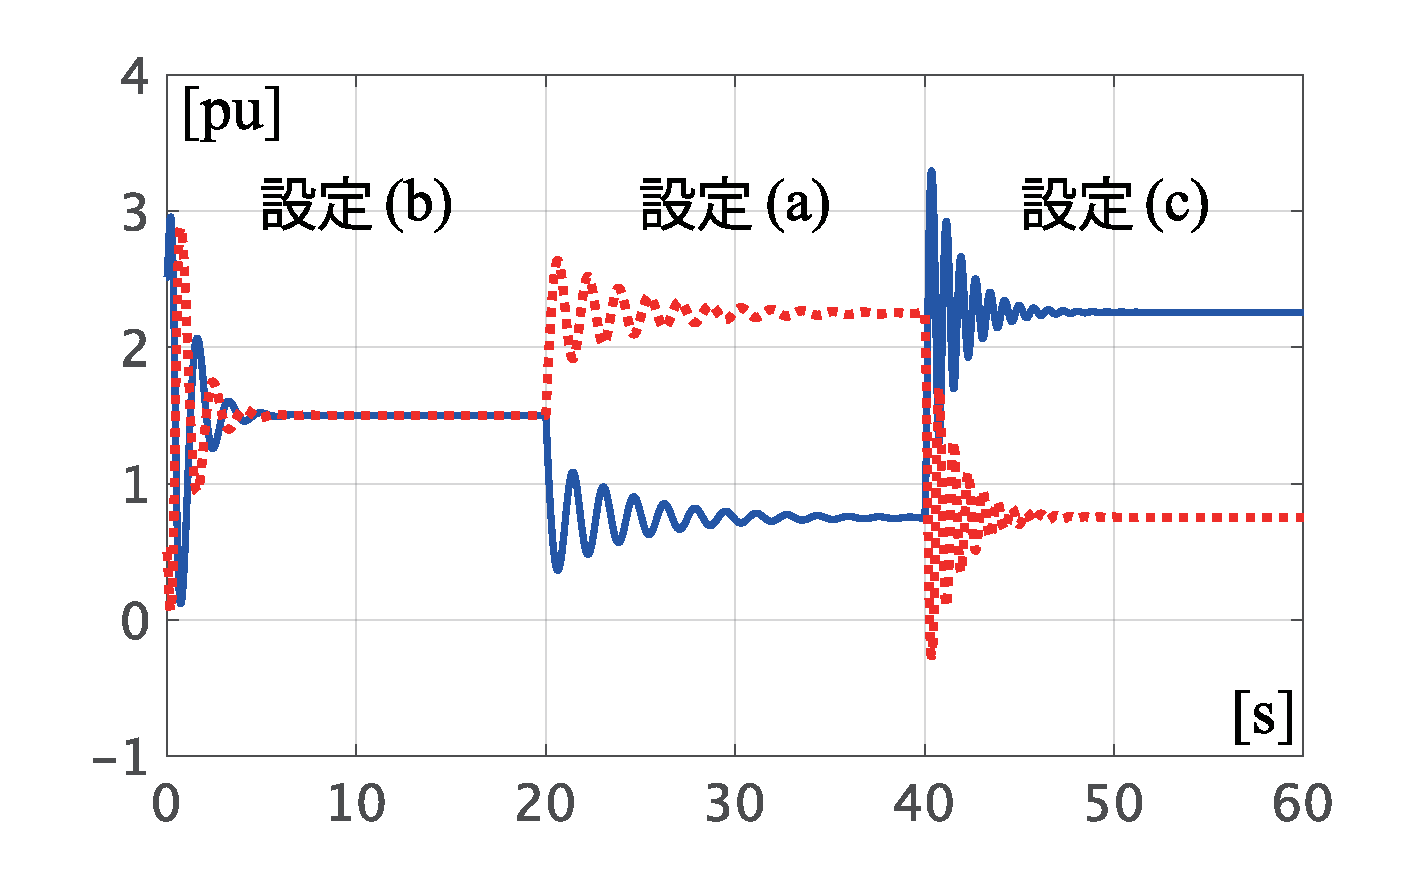
\includegraphics[width = 1.0\linewidth]{figs/varyalphaP}
    \subcaption{ Blue solid line: $P_1$, Red dashed line: $P_3$. }
  \end{minipage}
  \begin{minipage}{0.49\linewidth}
    \centering
    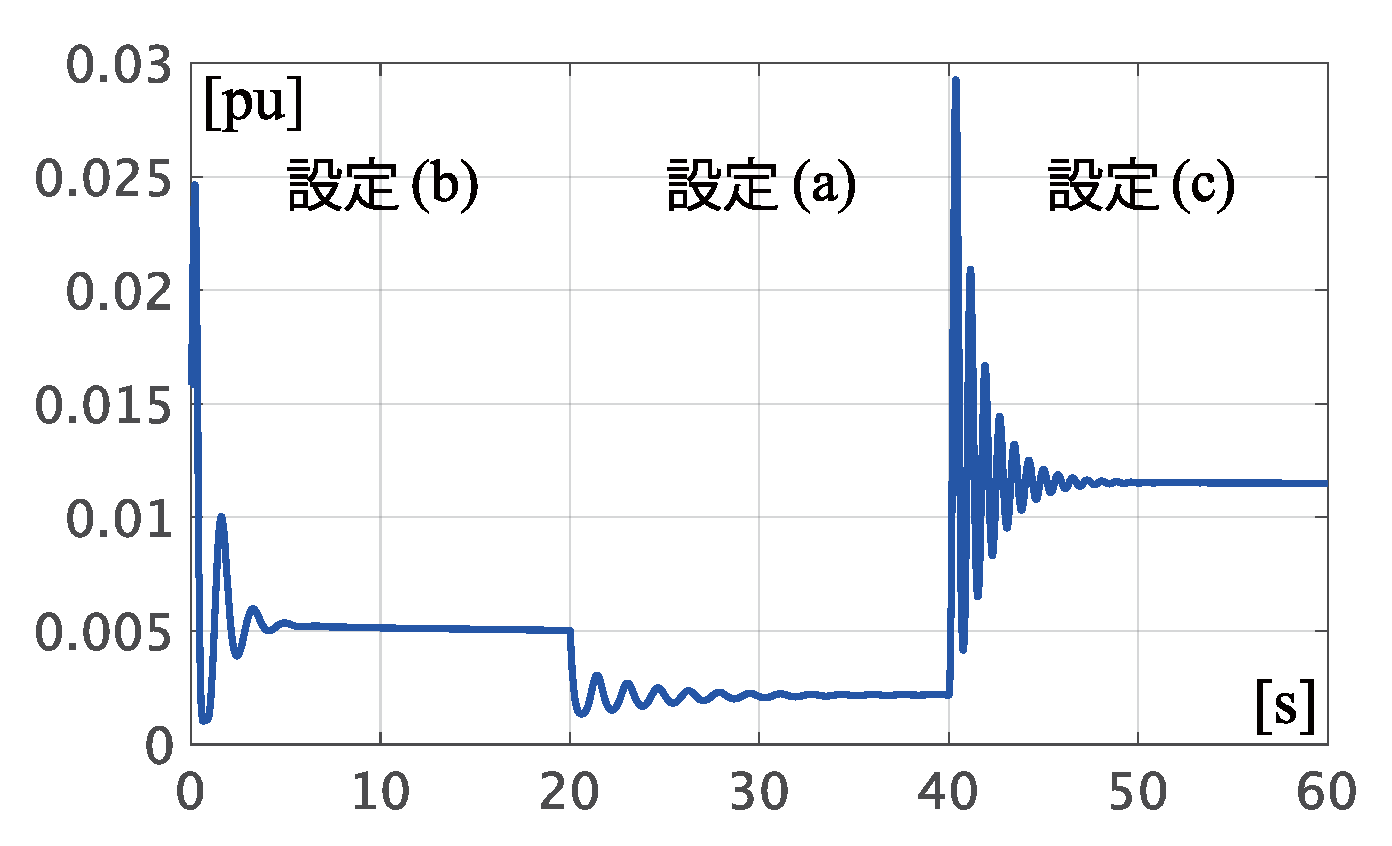
\includegraphics[width = 1.0\linewidth]{figs/varyalphaloss}
    \subcaption{Transmission loss $P_1+P_2+P_3$.}
  \end{minipage}
  \medskip
  \caption{\textbf{Time response of effective power to changes in contribution factor} }
  \label{fig:agcPvary}
  }
\medskip
\end{figure}


As shown in the Example \ref{ex:pfvary}, by adjusting the participation factor of the broadcast-type PI controller, the achieved steady power flow distribution can be changed.
At this time, the size of transmission loss and necessary power generation cost for each steady power flow distribution change.
Therefore, by appropriately controlling the participation factor, more economic system operation can be achieved.
However, since the steady power flow distribution with low economic cost is not necessarily an equilibrium point with a high degree of stability, tradeoff between economy and stability must be appropriately considered.

\section{Mathematical stability analysis of a frequency stabilization control system\advanced}\label{sec:mathnpas}

\subsection{The target electrical power system model\advanced}\label{sec:objmod}

\smallskip
\subsubsection{Assumptions for the electrical power system model and the automatic generation control}

In Section \ref{sec:stalin}, we assumed that the electrical power system model is near a steady power flow distribution, derived a linear approximation model, and analyzed necessary and adequate conditions for the small signal stability.
In this Section, we use a concept of passivity for a nonlinear system and analyze the frequency stability of an electrical power system model described as a differential-algebraic equation system.
Specifically, we consider the stability of an entire feedback control system where the automatic generation control is incorporated, and conduct a stability analysis with the following assumptions.

\begin{itemize}
\item All generators are expressed with the generator model of Equation (\ref{eq:lmodelsagc}). However, it is assumed that the field voltage of each generator is set to a constant.
\item All loads are expressed with the constant power model of Equation \ref{eq:contpwmod}.
\item For algebraic equations for the power grid of Equation \ref{eq:PQVgenagc}, conductance of all transmission lines is assumed to be 0.
\item For the broadcast-type PI controller of Equation (\ref{eq:agccon}), automatic generation control is performed.
However, it is assumed that $\alpha_i$ and $\beta_i$ are equal for all $i\in \mathcal{I}_{\rm G}$ for the weight of the participation factor and
frequency deviation.
\end{itemize}

The first and second assumptions mean that a standard model is considered for generators and loads.
The third assumption on the power grid means that the transmission loss is 0, which is essential in performing a mathematical stability analysis.
In fact, many papers have pointed out that when there is transmission loss, stability analysis of the electrical power system model must rely on a numerical method \cite{narasimhamurthi1984existence,chang1995direct,chiang2011direct,yang2019distributed}.
The fourth assumption is necessary for the input/output properties of the broadcast-type PI controller to be passive.
If participation factor $\alpha_i$ is positive for at least one $i\in \mathcal{I}_{\rm G}$, several coefficients can be 0.

As shown by the analysis of Section \ref{sec:phsync},
\begin{itemize}
\item The frequency deviation of all generators become equalize under a steady power flow distribution.
\end{itemize}
The following frequency stability analysis assumes this fact.
Specifically, for one integrator included in the broadcast-type PI controller to make the steady frequency deviation of all generators 0, a property is necessary whereby the above-described frequency deviation automatically synchronizes.

\smallskip
\subsubsection{Expression by feedback system of an electrical power system with automatic generation control}

Similar to the discussion of Section \ref{sec:linpasana}, let us consider describing the electrical power system model as a feedback system of two subsystems.
The first subsystem is:
\begin{align}\label{eq:sys1}
\mathds{F}:
\simode{
M \Delta \dot{\omega}&= 
- 
D
\Delta\omega 
 + 
u_{\mathds{F}}
+P_{{\rm mech}}^{\star}
\\
y_{\mathds{F}}&= \omega_0 \Delta\omega 
}
\end{align}
$\Delta\omega$ is a vector with $\Delta\omega_i$ in a column, while $M$ and $D$ are vectors where $M_i$ and $D_i$ are placed diagonally.
$P_{{\rm mech}}^{\star}$ is a vector with $P_{{\rm mech}i}^{\star}$.
$\mathds{F}$ is equal to the mechanical system in Section \ref{sec:linpasana} excluding the difference in the constant vector $P_{{\rm mech}}^{\star}$.
The second subsystem expresses the electrical subsystem of Section \ref{sec:linpasana} as a nonlinear differential-algebraic equation system:
\begin{subequations}\label{eq:sys2G}
\begin{align}\label{eq:sys2}
\mathds{G}_i : 
\simode{ 
\dot{\delta}_i &= u_{\mathds{G}_i}
\\
\taudi \dot{E}_i & = 
 -\tfrac{ \Xsi }{ \Xti }E_i
+\left(
\tfrac{ \Xsi }{ \Xti }-1
\right)
|\bm{V}_i| \sfcos (\delta_i - \angle \bm{V}_i ) 
+ V_{{\rm field}i}^{\star}
\\
y_{\mathds{G}_i}&= \tfrac{E_i |\bm{V}_i|}{ \Xti} \sfsin (\delta_i - \angle \bm{V}_i)
}
\end{align}
The voltage phasor of the bus bars in Equation \ref{eq:sys2} must simultaneously satisfy simultaneous equations related to all generator buses:
\begin{align}\label{eq:gVeq}
\simode{
P_i &=
\sum_{j=1}^{N} B_{ij} |\bm{V}_i| |\bm{V}_j| \sfsin(\angle \bm{V}_i -\angle \bm{V}_j)
\\
Q_i &= 
 -\sum_{j=1}^{N} B_{ij} |\bm{V}_i| |\bm{V}_j| \sfcos(\angle \bm{V}_i -\angle \bm{V}_j)
}\qquad
i \in \mathcal{I}_{\rm G}
\end{align}
and simultaneous equations related to all load bus bars:
\begin{align}\label{eq:lVeq}
\simode{
&P_{{\rm load}i}^{\star} =
\sum_{j=1}^{N} B_{ij} |\bm{V}_i| |\bm{V}_j| \sfsin(\angle \bm{V}_i -\angle \bm{V}_j)
\\
&Q_{{\rm load}i}^{\star} = 
-\sum_{j=1}^{N} B_{ij} |\bm{V}_i| |\bm{V}_j| \sfcos(\angle \bm{V}_i -\angle \bm{V}_j)
}\qquad
i \in \mathcal{I}_{\rm L}
\end{align}
\end{subequations}
The active power $P_i$ and reactive power $Q_i$ of Equation \ref{eq:gVeq} are defined by Equation \ref{eq:PQoutagc}.
$B_{ij}$ expresses the $(i,j)$th element of the susceptance matrix $B$, which is the imaginary part of the admittance matrix $\bm{Y}$.
Below, for all generator buses $i \in \mathcal{I}_{\rm G}$, we consider a summary of Equation \ref{eq:sys2} to Equation \ref{eq:lVeq} as one subsystem and express it as the electrical subsystem $\mathds{G}$.

In addition, the dynamic characteristics of the broadcast-type PI controller of Equation (\ref{eq:agccon}) are expressed as:
\begin{align}\label{eq:condsK}
\mathds{K}: \simode{
\dot{\xi}&=  h^{\sf T} u_{\mathds{K}} \\
y_{\mathds{K}} &= h \left(k_{\rm P} h^{\sf T}u_{\mathds{K}} +  k_{\rm I} \xi \right)
}
\end{align}
where $h$ is a column vector with $\alpha_i$.
At this time, if the input and output of the above subsystems $\mathds{F}$ and $\mathds{G}$ and the controller $\mathds{K}$ are combined as follows:
\begin{subequations}\label{eq:connds}
\begin{align}
u_{\mathds{F}} = - y_{\mathds{K}} + v_{\mathds{F}}&
,\qquad u_{\mathds{K}} = \frac{1}{\omega_0} y_{\mathds{F}}	\label{eq:connds1}
\\
u_{\mathds{G}} = y_{\mathds{F}}&
,\qquad
v_{\mathds{F}} = - y_{\mathds{G}}		\label{eq:connds2}
\end{align}
\end{subequations}
we can express an entire feedback control system that incorporates the automatic generation control.
However, $u_{\mathds{G}}$ and $y_{\mathds{G}}$ are vectors with $u_{\mathds{G}_i}$ and $y_{\mathds{G}_i}$.
\FIGref{fig:nonlinBD} shows a block diagram of the entire feedback control system.
Please note that the block of “electric power balance equation” includes unknown model parameters, such as consumed electric power of loads and admittance of transmission lines. 

\begin{figure}[t]
\centering
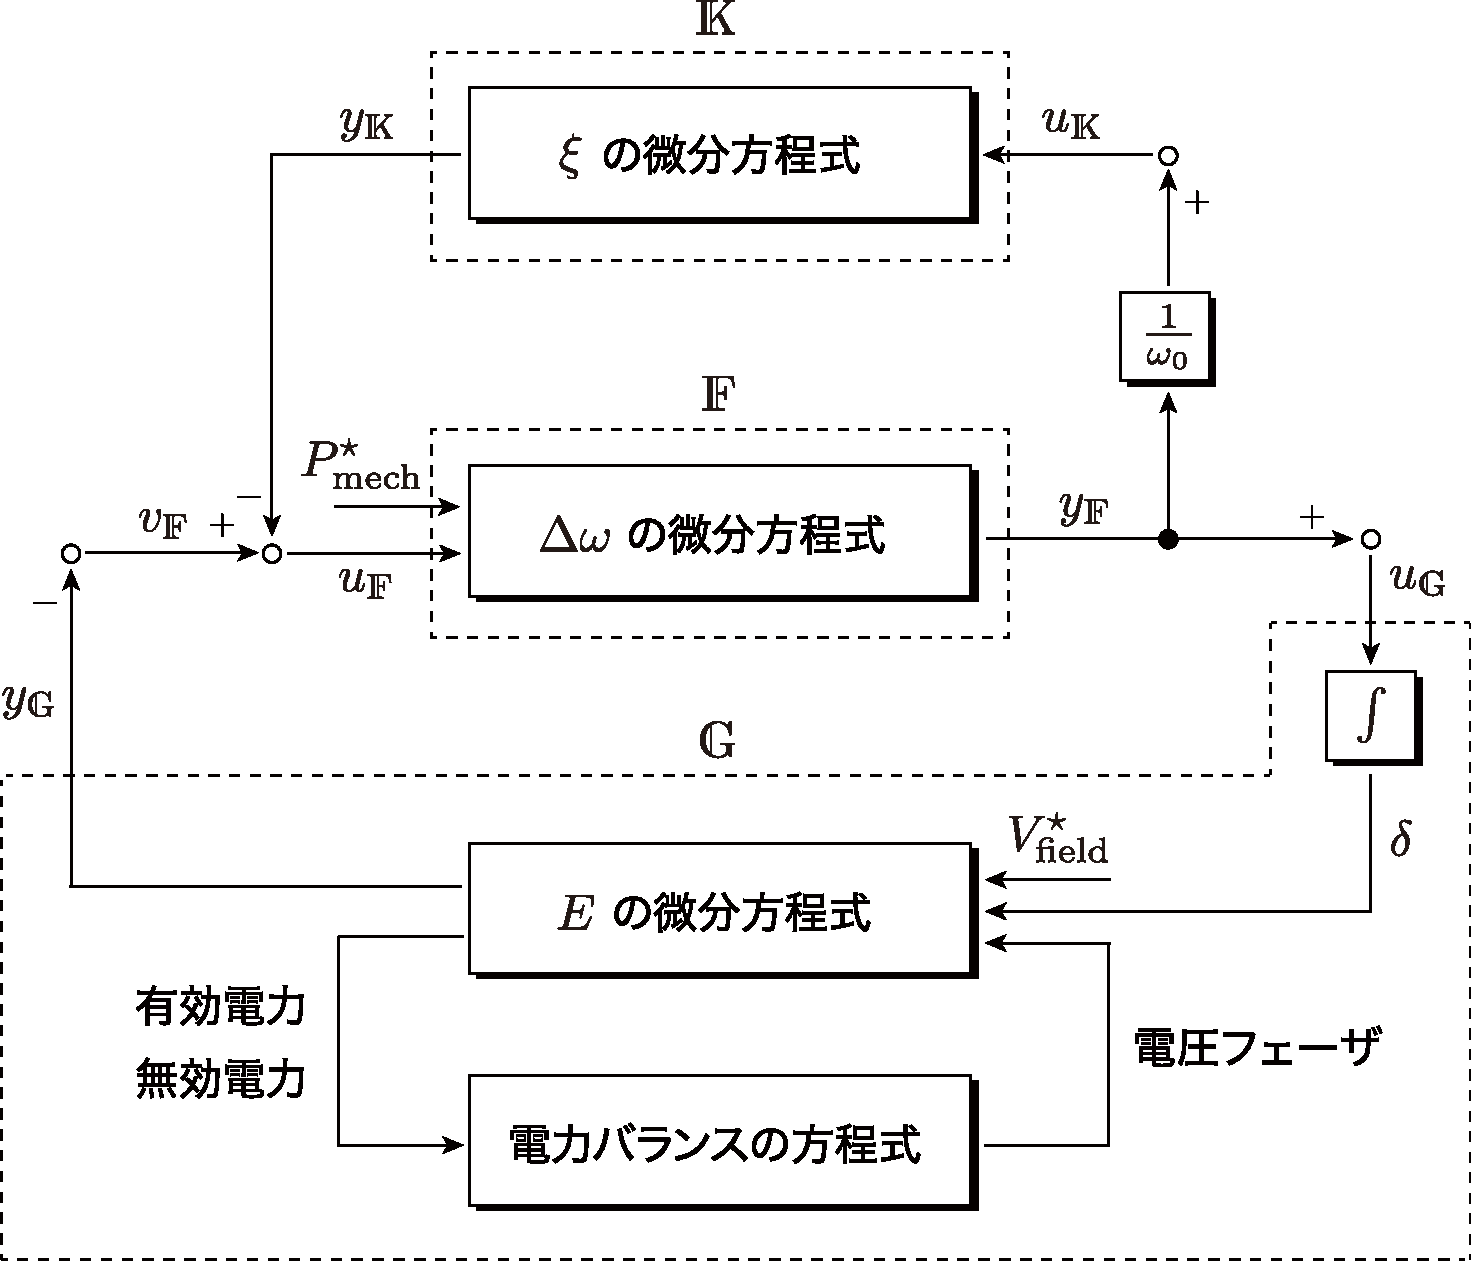
\includegraphics[width = .85\linewidth]{figs/nonlinBD}
\medskip
\caption{\textbf{Feedback control system incorporating automatic power generation control}}
\label{fig:nonlinBD}
\medskip
\end{figure}



\subsection{Passivity independent of the equilibrium point of the electrical power system\advanced}

\smallskip
\subsubsection{Passivity independent of the equilibrium point}

The discussion of Section \ref{sec:linpasana} was an analysis by the linear approximation model; thus, the internal state asymptotically converging to 0 expressed the asymptotic convergence to a specific steady power flow distribution of the original nonlinear model.
On the other hand, with the electrical power system model expressed as a nonlinear differential-algebraic equation system, the internal state does not become 0 even with a steady power flow distribution where the supply and demand of electric power are balanced.
Furthermore, the steady power flow distribution itself changes based on the setting of mechanical torque and so on.
Therefore, a stability analysis independent of the choice of each steady power flow distribution (equilibrium point) is desirable. A concept proposed by control systems engineering to perform this analysis is called \textbf{equilibrium-independent passivity} \cite{hines2011equilibrium,simpson2019equilibrium}. Depending on the paper, it is also called \textbf{shifted passivity}. Its definition is as follows:

\begin{定義}[Equilibrium-independent passivity]\label{def:eipassive}
Let us consider a nonlinear system:
\begin{align}\label{eq:nlsig}
\Sigma: \simode{
E\dot{x} &= f(x) + Bu + R d^{\star}\\
y &= h(x)
}
\end{align}
$f:\mathcal{X} \rightarrow \mathbb{R}^{n}$ and $h:\mathcal{X} \rightarrow \mathbb{R}^{m}$ are smooth functions, and $B \in \mathbb{R}^{n\times m}$, $E \in \mathbb{R}^{n\times n}$, and $R \in \mathbb{R}^{n\times p}$ are matrices.
\begin{align*}%\label{eq:asbleq}
\mathcal{E}_{\Sigma} :=
\left\{
x^{\star} \in \mathcal{X}: 
\mbox{$0 = f(x^{\star})+B u^{\star}+ R d^{\star}$を満たす$u^{\star}$が存在する}
\right\}
\end{align*}
$\Sigma$ of Equation \ref{eq:nlsig} expresses:
\begin{align*}%\label{eq:eiconpv}
\frac{d}{dt} W_{x^{\star}} \bigl( x(t) \bigr) \leq \bigl(u(t)-u^{\star}\bigr)^{\sf T} \bigl(y(t)-y^{\star}\bigr)
,\qquad
\forall t \geq 0
\end{align*}
of the differential-algebraic equation system.
If applied to an electrical subsystem $\mathds{G}$, $x_1$ is a vector with all $\delta_i$ and $E_i$, while $x_2$ is a vector with all $|\bm{V}_i|$ and $\angle \bm{V}_i$.
On the other hand, when $E$ is nonsingular, it expresses an ordinary differential equation system, such as a mechanical subsystem $\mathds{F}$ of Equation \ref{eq:sys1}.
Such a system expression is called a \textbf{descriptor representation}.
\begin{align*}%\label{eq:uystar}
u^{\star} := -(B^{\sf T}B)^{-1}B^{\sf T} \bigl\{f(x^{\star}) + R d^{\star} \bigr\}
,\qquad
y^{\star} := h(x^{\star}) 
\end{align*}
と表している。
特に,上記の半正定値関数$W_{x^{\star}}(x)$に加えて
\begin{align*}%\label{eq:eiconosp}
\frac{d}{dt} W_{x^{\star}} \bigl( x(t) \bigr) \leq \bigl(u(t)-u^{\star}\bigr)^{\sf T} \bigl(y(t)-y^{\star}\bigr)
-\rho \bigl\|y(t)-y^{\star} \bigr\|^2
,\qquad
\forall t \geq 0
\end{align*}
For an arbitrary input $u $ for each and every equilibrium point $x^{\star} \in \mathcal{E}_{\Sigma}$ where $W_{x^{\star}} (x^{\star})$ is 0, $\Sigma$ is called \textbf{passive independent of the equilibrium point}.
Steady input and output for the equilibrium point $x^{\star}$ are expressed as:
\end{定義}

With definition \ref{def:eipassive}, we can interpret that the passivity is defined with the equilibrium point $x^{\star} \in \mathcal{E}_{\Sigma}$ of the system as the reference.
With a category of a linear system, as long as the system does not have a zero eigenvalue, it is an equivalent definition to the passivity of Section \ref{sec:linpasana}.
The above function $W_{x^{\star}}(x)$ is called a storage function in the same manner as the regular passivity.
Please note that this storage function $W_{x^{\star}}(x)$ is an implicit function of the equilibrium point $x^{\star}$.  In the literature \cite{simpson2019equilibrium}, if the system is passive independent of the equilibrium point , its storage function can be expressed with:

\begin{COLUMN}
\noindent \textbf{ディスクリプタ形式}:
Matrix $E$ was introduced to express an electrical subsystem $\mathds{G}$ of Equation (\ref{eq:sys2G}), which is a differential-algebraic equation system.
Specifically, if:
\[
E=\mat{
I & 0 \\
0 & 0\\ 
}
\]
$\Sigma$ of Equation \ref{eq:nlsig} expresses:
\begin{align*}
\simode{
\dot{x}_1 &= f_1(x_1,x_2) + B_1u + R_1 d^{\star}\\
0 &= f_2(x_1,x_2) \\
y &= h(x_1,x_2)
}
\end{align*}
of the differential-algebraic equation system.
If applied to an electrical subsystem $\mathds{G}$, $x_1$ is a vector with all $\delta_i$ and $E_i$, while $x_2$ is a vector with all $|\bm{V}_i|$ and $\angle \bm{V}_i$.
On the other hand, when $E$ is nonsingular, it expresses an ordinary differential equation system, such as a mechanical subsystem $\mathds{F}$ of Equation \ref{eq:sys1}.
Such a system expression is called a \textbf{descriptor representation}. 
\end{COLUMN}

\red{Translated with DeepL}
In the literature \cite{simpson2019equilibrium}, if the system is passive independent of the equilibrium point, its accumulation function is a function $U(x)$ given by:
\begin{align}\label{eq:paraW}
W_{x^{\star}}(x) = U(x) - U(x^{\star}) - \nabla U^{\sf T}(x^{\star}) (x-x^{\star})
\end{align}
With definition \ref{def:eipassive}, the storage function $W_{x^{\star}}(x)$ of Equation \ref{eq:paraW} being a positive semi-definite function is a condition.
Specifically, the following must hold:
\begin{align}\label{eq:Uineqst}
U(x) \geq  U(x^{\star}) + \nabla U^{\sf T}(x^{\star}) (x-x^{\star})
\end{align}
If this inequality holds for an arbitrary set $(x,x^{\star}) \in \mathcal{X} \times \mathcal{X}$, $W_{x^{\star}}(x)$ is a positive semi-definite function for each and every equilibrium point $x^{\star} \in \mathcal{E}_{\Sigma}$.
The inequality of Equation \ref{eq:Uineqst} expresses that $U(x)$ is a \textbf{convex function}

\begin{COLUMN}
\noindent \textbf{Convex function}:
If the following is true for a set of two arbitrary points $(x,y)$ selected from a defined range for the function $f(x)$:
\[
f\bigl(
\theta x + (1-\theta) y
\bigr)
\leq \theta f(x) + (1- \theta) f(y)
,\qquad
\forall \theta \in [0,1]
\]
$f(x)$ is called a \textbf{convex function}. Specifically, when $f(x)$ is differentiable, the condition for $f(x)$ to be a convex function is that the following is true for a set of two arbitrary points $(x,y)$:
\[
f(x) \geq f(y) + \nabla f^{\sf T}(y)(x-y)
\]

\smallskip
\noindent \textbf{Bregman distance}:
In statistics, the amount on the right side of Equation \ref{eq:paraW} for a convex function $U(x)$ is called the \textbf{Bregman distance} related to $U(x)$ of $x$ and $x^{\star}$ \cite{bregman1967relaxation}.
When $U(x)$ is $\|x\|^2$, $W_{x^{\star}}(x)$ is consistent with Euclidean distance $\|x-x^{\star}\|^2$.
\end{COLUMN}



\smallskip
\subsubsection{Analysis of a mechanical subsystem}

As shown in Section \ref{sec:linpasana}, the mechanical subsystem $\mathds{F}$ is strictly passive.
Similarly, confirm that $\mathds{F}$ of Equation \ref{eq:sys1} is strictly passive and independent of the equilibrium point.
First, write the mechanical subsystem as follows:
\begin{align}
\mathds{F}: \simode{
\dot{x}_{\mathds{F}} & = A_{\mathds{F}} x_{\mathds{F}} + B_{\mathds{F}} u_{\mathds{F}} 
+ R_{\mathds{F}} d_{\mathds{F}}^{\star} \\
y_{\mathds{F}} &= C_{\mathds{F}} x_{\mathds{F}}
}
\end{align}
State $x_{\mathds{F}}$ is a vector with $\Delta \omega_i$, and $u_{\mathds{F}}$ and $y_{\mathds{F}}$ are vectors with $u_{\mathds{F}_i}$ and $y_{\mathds{F}_i}$.  $d_{\mathds{F}}^{\star}$ expresses $P_{\rm mech}^{\star}$, and the system matrix is:
\[
A_{\mathds{F}} := -M^{-1}D,\qquad
B_{\mathds{F}} := M^{-1},\qquad
R_{\mathds{F}} := M^{-1},\qquad
C_{\mathds{F}} := \omega_0 I
\]
Matrices $M$ and $D$ are matrices with $M_i$ and $D_i$ in diagonal. We select a storage function for the arbitrarily selected equilibrium point $x^{\star}_{\mathds{F}} \in \mathcal{E}_{\mathds{F}}$:
\begin{align}\label{eq:WxFst}
W_{x^{\star}_{\mathds{F}}}(x_{\mathds{F}})
= \frac{\omega_0}{2}
(x_{\mathds{F}} -x^{\star}_{\mathds{F}})^{\sf T}
M
(x_{\mathds{F}} -x^{\star}_{\mathds{F}})
\end{align}
However, $(x^{\star}_{\mathds{F}},u^{\star}_{\mathds{F}},y^{\star}_{\mathds{F}})$ related to the equilibrium point satisfies:
\begin{align}\label{eq:xFsteady}
0=
A_{\mathds{F}} x^{\star}_{\mathds{F}}
+
B_{\mathds{F}} u^{\star}_{\mathds{F}}
+ R_{\mathds{F}} d_{\mathds{F}}^{\star}
,\qquad
y^{\star}_{\mathds{F}} = C_{\mathds{F}} x^{\star}_{\mathds{F}}
\end{align}
If expressing in the form of Equation \ref{eq:paraW}, with:
\[
U_{\mathds{F}}(x_{\mathds{F}}):= \frac{\omega_0}{2} x_{\mathds{F}}^{\sf T} M x_{\mathds{F}}
\]
the storage function can be expressed as:
\[
W_{x^{\star}_{\mathds{F}}}(x_{\mathds{F}}) = U_{\mathds{F}}(x_{\mathds{F}}) 
- U_{\mathds{F}}(x^{\star}_{\mathds{F}}) 
- \nabla U^{\sf T}_{\mathds{F}}(x^{\star}_{\mathds{F}}) (x_{\mathds{F}}-x^{\star}_{\mathds{F}})
\]
A gradient function of this storage function is:
\begin{align*}%\label{eq:nabW}
\nabla W_{x^{\star}_{\mathds{F}}}(x_{\mathds{F}}) = \omega_0 M (x_{\mathds{F}} -x^{\star}_{\mathds{F}})
\end{align*}
thus, the time derivative of the storage function can be evaluated as:
\begin{align}\label{eq:tdFds}
\spliteq{
\frac{d}{dt} W_{x^{\star}_{\mathds{F}}} \bigl( x_{\mathds{F}}(t) \bigr) 
&= 
\nabla W_{x^{\star}_{\mathds{F}}}^{\sf T}\left( x_{\mathds{F}}(t) \right) \dot{x}_{\mathds{F}}(t) \\
&= 
\nabla W_{x^{\star}_{\mathds{F}}}^{\sf T}\left( x_{\mathds{F}}(t) \right)
 \left\{
A_{\mathds{F}} \left( x_{\mathds{F}}(t) -x^{\star}_{\mathds{F}} \right)
+
B_{\mathds{F}} \left( u_{\mathds{F}}(t) -u^{\star}_{\mathds{F}} \right)
\right\}
\\
& \leq \textstyle
(y_{\mathds{F}}(t) -y^{\star}_{\mathds{F}})^{\sf T}
(u_{\mathds{F}}(t) -u^{\star}_{\mathds{F}})
 - \tfrac{\sfmin \left\{ D_i \right\}}{\omega_0}
\|y_{\mathds{F}}(t) -y^{\star}_{\mathds{F}}\|^2
}
\end{align}
To derive the second equal sign, the relationship of Equation \ref{eq:xFsteady} was used.


\smallskip
\subsubsection{Analysis of a feedback system of a mechanical subsystem and automatic generation controller}

In the same way as the mechanical subsystem, the passivity of the broadcast-type PI controller of Equation \ref{eq:condsK} can be shown as well.
If we define the storage function as: 
\begin{align}\label{eq:Wxist}
W_{\xi^{\star}}(\xi) := \frac{1}{2} k_{\rm I} (\xi-\xi^{\star} )^2
\end{align}
its time derivative can be evaluated as:
\begin{align}\label{eq:tdKds}
\spliteq{
\frac{d}{dt} W_{\xi^{\star}} \bigl( \xi(t) \bigr) 
&=
(y_{\mathds{K}} - y_{\mathds{K}}^{\star})^{\sf T} (u_{\mathds{K}} - u_{\mathds{K}}^{\star})
- k_{\rm P} u_{\mathds{K}}^{\sf T} hh^{\sf T} u_{\mathds{K}} \\
& \leq (y_{\mathds{K}} - y_{\mathds{K}}^{\star})^{\sf T} (u_{\mathds{K}} - u_{\mathds{K}}^{\star})
}
\end{align}
We used the fact that the following holds for $(\xi^{\star},u_{\mathds{K}}^{\star},y_{\mathds{K}}^{\star})$ at the equilibrium point:
\begin{align}\label{eq:Kdseq}
\simode{
0 &=  h^{\sf T} u_{\mathds{K}}^{\star} \\
y_{\mathds{K}}^{\star} &= h \left(k_{\rm P} h^{\sf T}u_{\mathds{K}}^{\star} +  k_{\rm I} \xi^{\star} \right)
}
\end{align}

In control systems engineering, it is known that a negative feedback system of two passive systems will be passive again.
Based on this fact, the feedback connection of the mechanical subsystem $\mathds{F}$ of Equation \ref{eq:sys1} and the broadcast-type PI controller $\mathds{K}$ of Equation \ref{eq:condsK}:
\begin{align}\label{eq:sysFKds}
\mathds{F}_+:
\simode{
M \Delta \dot{\omega}&= 
- 
D
\Delta\omega 
- h \left(k_{\rm P} h^{\sf T}\Delta\omega  +  k_{\rm I} \xi \right)  + P_{{\rm mech}}^{\star} + v_{\mathds{F}}
\\
\dot{\xi} &= h^{\sf T}\Delta\omega\\
y_{\mathds{F}}&= \omega_0 \Delta\omega 
}
\end{align}
can be shown to be strictly passive and independent of the equilibrium point.
In actual fact, by combining the inequality of Equations \ref{eq:tdFds} and \ref{eq:tdKds}, the following is obtained:
\begin{align}\label{eq:disineqFp}
\spliteq{
& \frac{d}{dt}  \left\{
W_{x^{\star}_{\mathds{F}}}  \bigl( x_{\mathds{F}}(t) \bigr) 
+
\omega_0
W_{\xi^{\star}} \bigl( \xi(t) \bigr) 
\right\} \\
& \hspace{3em} \leq 
(y_{\mathds{F}}(t) -y^{\star}_{\mathds{F}})^{\sf T}
(v_{\mathds{F}}(t) -v^{\star}_{\mathds{F}})  
- \tfrac{\sfmin \left\{ D_i \right\}}{\omega_0}
\|y_{\mathds{F}}(t) -y^{\star}_{\mathds{F}}\|^2
}
\end{align}
We used the input-output relationship of Equation \ref{eq:connds1}.

If we connect $\mathds{F}_+$ of Equation \ref{eq:sysFKds} and $\mathds{G}$ of Equation (\ref{eq:sys2G}) from the input-output relationship of Equation \ref{eq:connds2}, the entire feedback control system with the automatic generation control can be expressed.
Based on this fact, we analyse the equilibrium-independent passivity of $\mathds{G}$.

\smallskip
\subsubsection{Analysis of an electrical subsystem}

Let us analyze the equilibrium-independent passivity of the electrical subsystem $\mathds{G}$ of Equation (\ref{eq:sys2G}).
Below, we express a column vector with all time variables $\delta_i$,$E_i$, $|\bm{V}_i|$, $\angle \bm{V}_i$ related to the generator buses and load bus bars of $\mathds{G}$ is expressed as $x_{\mathds{G}}$.
With this description, we define a potential energy function as:
\begin{align}\label{eq:potWx}
\spliteq{
U_{\mathds{G}}(x_{\mathds{G}})  := 
&  \sum_{i=1}^n
\left\{
\frac{ \Xsi E_i^2 }{2 \Xti ( \Xsi - \Xti )}  
- 
\frac{E_i |\bm{V}_i|}{ \Xti } \sfcos (\delta_i - \angle \bm{V}_i)
+\frac{|\bm{V}_i|^2}{2 \Xti }
\right\}
\\
- & 
\sum_{i=n+1}^{n+m}
\left\{
 P_{{\rm load}i}^{\star} \angle \bm{V}_i
+ Q_{{\rm load}i}^{\star} \ln \left|\bm{V}_i \right|
\right\} \\
- & \sum_{i=1}^{N}
\sum_{j=1}^{N} \frac{B_{ij} }{2} |\bm{V}_i| |\bm{V}_j| \sfcos(\angle \bm{V}_i -\angle \bm{V}_j)
%\left\{
% \frac{B_{ii} }{2} |\bm{V}_i|^2  
%+ \sum_{j=1,j\neq i}^{N} \frac{B_{ij} }{2} |\bm{V}_i| |\bm{V}_j| \sfcos(\angle \bm{V}_i -\angle \bm{V}_j)
%\right\}
}
\end{align}
This potential energy function, for example, is used to analyze the stability of an electrical power system consisting of a uniaxial generator model and constant electric power load model in \cite{tsolas1985structure,varaiya1985direct,chiang2011direct}.
A candidate for the storage function is structured as follows based on the expression of Equation \ref{eq:paraW}: 
\begin{align}\label{eq:stops}
W_{x^{\star}_{\mathds{G}}}(x_{\mathds{G}}) = U_{\mathds{G}}(x_{\mathds{G}}) 
- U_{\mathds{G}}(x^{\star}_{\mathds{G}}) 
- \nabla U_{\mathds{G}}^{\sf T}(x^{\star}_{\mathds{G}}) (x_{\mathds{G}}-x^{\star}_{\mathds{G}})
\end{align}
Its gradient function is:
\[
\nabla W_{x^{\star}_{\mathds{G}}}(x_{\mathds{G}}) =
\nabla U_{\mathds{G}}(x_{\mathds{G}}) 
- \nabla U_{\mathds{G}}(x^{\star}_{\mathds{G}}) 
\]
To calculate the time derivative of the storage function, we obtain the gradient function of the potential energy function.
First, if we calculate the partial differential related to $\delta_i$ and $E_i$ of $ U_{\mathds{G}}(x_{\mathds{G}}) $:
\begin{align*}
\frac{\partial U_{\mathds{G}}}{\partial \delta_i}(x_{\mathds{G}}) &= \frac{E_i |\bm{V}_i|}{ \Xti } \sfsin (\delta_i - \angle \bm{V}_i) ,
\\
\frac{\partial U_{\mathds{G}}}{\partial E_i} (x_{\mathds{G}})&= - \frac{1}{ \Xsi - \Xti }
\left\{
-\frac{ \Xsi }{ \Xti }E_i
+\left(
\frac{ \Xsi }{ \Xti }-1
\right)
|\bm{V}_i| \sfcos (\delta_i - \angle \bm{V}_i ) 
\right\}
\end{align*}
Therefore, if each variable follows the differential-algebraic equation of Equation (\ref{eq:sys2G}), because of Equation \ref{eq:sys2}, the following is true for all $i\in \mathcal{I}_{\rm G}$:
\begin{align*}
\frac{\partial U_{\mathds{G}}}{\partial \delta_i}(x_{\mathds{G}})  = y_{\mathds{G}_i}
,\qquad
\frac{\partial U_{\mathds{G}}}{\partial E_i} (x_{\mathds{G}})= 
\frac{V_{{\rm field}i}^{\star} - \taudi\dot{E}_i  }{ \Xsi - \Xti }
\end{align*}
Also, for $i\in \mathcal{I}_{\rm G}$, the partial derivative of the potential energy function with respect to the voltage phasor variable is:
\begin{align*}
\spliteq{
\frac{\partial U_{\mathds{G}}}{\partial |\bm{V}_i| }(x_{\mathds{G}}) &= 
-
\sum_{j=1}^{N} B_{ij}  |\bm{V}_j| \sfcos(\angle \bm{V}_i -\angle \bm{V}_j)- \frac{Q_i}{|\bm{V}_i|}
\\
\frac{\partial U_{\mathds{G}}}{\partial \angle \bm{V}_i } (x_{\mathds{G}})&= 
\sum_{j=1}^{N}
B_{ij} |\bm{V}_i| |\bm{V}_j| \sfsin(\angle \bm{V}_i -\angle \bm{V}_j)
-
P_i
}
\end{align*}
Therefore, we can see that because of Equation \ref{eq:gVeq}, these are all 0.
Similarly, from Equation \ref{eq:lVeq}, we can see that the following is 0 for $i\in \mathcal{I}_{\rm L}$:
\begin{align*}
\spliteq{
\frac{\partial U_{\mathds{G}}}{\partial |\bm{V}_i| }(x_{\mathds{G}}) &= 
- \sum_{j=1}^{N} B_{ij}  |\bm{V}_j| \sfcos(\angle \bm{V}_i -\angle \bm{V}_j)
 -  \frac{Q_{{\rm load}i}^{\star}}{|\bm{V}_i|}
\\
\frac{\partial U_{\mathds{G}}}{\partial \angle \bm{V}_i } (x_{\mathds{G}})&= 
\sum_{j=1}^{N} B_{ij} |\bm{V}_i| |\bm{V}_j| \sfsin(\angle \bm{V}_i -\angle \bm{V}_j)
-
P_{{\rm load}i}^{\star}
}
\end{align*}
Thus, the following holds for all $i\in \mathcal{I}_{\rm G} \cup \mathcal{I}_{\rm L}$:
\begin{align*}
\frac{\partial U_{\mathds{G}}}{\partial |\bm{V}_i| } (x_{\mathds{G}})= 0
,\qquad
\frac{\partial U_{\mathds{G}}}{\partial \angle \bm{V}_i } (x_{\mathds{G}})= 0
\end{align*}

\begin{subequations}\label{eq:eqeq}
Next, let us consider a set $(x^{\star}_{\mathds{G}},u^{\star}_{\mathds{G}},y^{\star}_{\mathds{G}})$ related to the steady state of $\mathds{G}$ in terms of $\nabla U_{\mathds{G}}(x^{\star}_{\mathds{G}}) $.
From the relationship of the equilibrium point, there are voltage phasor variables $(|\bm{V}_i^{\star}|, \angle \bm{V}_i^{\star})_{i\in \mathcal{I}_{\rm G} \cup \mathcal{I}_{\rm L} }$, and the following holds:
\begin{align}\label{eq:eqeqa}
&\simode{
0 & = u_{\mathds{G}_i}^{\star} \\
 0 & =
-\tfrac{ \Xsi }{ \Xti }E_i^{\star}
+\left(
\tfrac{ \Xsi }{ \Xti }-1
\right)
|\bm{V}_i^{\star}| \sfcos (\delta_i^{\star} - \angle \bm{V}_i^{\star} ) 
+V_{{\rm field}i}^{\star}
} \\
&\simode{
P_i^{\star} 
& =
\sum_{j=1}^{N} B_{ij} |\bm{V}_i^{\star}| |\bm{V}_j^{\star}| \sfsin(\angle \bm{V}_i^{\star} -\angle \bm{V}_j^{\star})
\\
Q_i^{\star} 
&=
 - \sum_{j=1}^{N} B_{ij} |\bm{V}_i^{\star}| |\bm{V}_j^{\star}| \sfcos(\angle \bm{V}_i^{\star} -\angle \bm{V}_j^{\star})
}
\end{align}
However, $ i \in \mathcal{I}_{\rm G} $, and the steady values of active power and reactive power are:
\begin{align*}%\label{eq:PQoutagcst}
P_i^{\star}  :=  \frac{E_i^{\star}  |\bm{V}_i^{\star} |}{ \Xti } 
\sfsin (\delta_i^{\star}  - \angle \bm{V}_i^{\star} ), \qquad
Q_i^{\star}  :=  \frac{ E_i^{\star} |\bm{V}_i^{\star} | }{ \Xti } 
\sfcos (\delta_i^{\star}  - \angle \bm{V}_i^{\star} )
-\frac{|\bm{V}_i^{\star} |^2}{ \Xti }
\end{align*}
In addition, $y_{\mathds{G}_i}^{\star}$ expresses $P_i^{\star}$.
Therefore, the following holds for $ i \in \mathcal{I}_{\rm G} $:
\begin{align*}
\frac{\partial U_{\mathds{G}}}{\partial \delta_i}(x^{\star}_{\mathds{G}}) = y_{\mathds{G}_i}^{\star}
,\qquad
\frac{\partial U_{\mathds{G}}}{\partial E_i}(x^{\star}_{\mathds{G}}) = 
\frac{V_{{\rm field}i}^{\star}  }{ \Xsi - \Xti }
\end{align*}
Similarly, since the following holds for all $ i \in \mathcal{I}_{\rm L} $:
\begin{align}
\simode{
&P_{{\rm load}i}^{\star}=
\sum_{j=1}^{N} B_{ij} |\bm{V}_i^{\star}| |\bm{V}_j^{\star}| \sfsin(\angle \bm{V}_i^{\star} -\angle \bm{V}_j^{\star}) 
\\
&Q_{{\rm load}i}^{\star}
=
-\sum_{j=1}^{N} B_{ij} |\bm{V}_i^{\star}| |\bm{V}_j^{\star}| \sfcos(\angle \bm{V}_i^{\star} -\angle \bm{V}_j^{\star})
}
\end{align}
\end{subequations}
The partial differential related to the voltage phasor variables of the bus bars becomes:
\begin{align*}
\frac{\partial U_{\mathds{G}}}{\partial |\bm{V}_i| }(x^{\star}_{\mathds{G}})= 0
,\qquad
\frac{\partial U_{\mathds{G}}}{\partial \angle \bm{V}_i } (x^{\star}_{\mathds{G}})= 0
\end{align*}
for all $i\in \mathcal{I}_{\rm G} \cup \mathcal{I}_{\rm L}$.
Because of the above calculation, the time derivative along the solution trajectory of storage function $\mathds{G}$ can be evaluated as:
\begin{align}\label{eq:disineqGds}
\spliteq{
\frac{d}{dt}W_{x^{\star}_{\mathds{G}}} \bigl(x_{\mathds{G}}(t) \bigr)
& =
\nabla W_{x^{\star}_{\mathds{G}}}^{\sf T} \bigl(x_{\mathds{G}}(t) \bigr)
\dot{x}_{\mathds{G}}(t) \\
&=
\sum_{i=1}^n
\left(
(u_{\mathds{G}_i}- u_{\mathds{G}_i}^{\star}) (y_{\mathds{G}_i}-y_{\mathds{G}_i}^{\star})
-
\frac{\taudi}{ \Xsi - \Xti }
\dot{E}_i^2
\right)\\
& \leq 
(y_{\mathds{G}}-y_{\mathds{G}}^{\star})^{\sf T} (u_{\mathds{G}}- u_{\mathds{G}}^{\star})
}
\end{align}
Because of Equation \ref{eq:eqeqa}, we used the fact that $u_{\mathds{G}}^{\star}$ is 0.
As such, we can see that the function $W_{x^{\star}_{\mathds{G}}}(x_{\mathds{G}})$ of Equation \ref{eq:stops} becomes the storage function against the equilibrium-independent passivity of the electrical subsystem $\mathds{G}$.
However, please note that the ranges of $x_{\mathds{G}}$ and $x_{\mathds{G}}^{\star}$ are limited to the range where $W_{x^{\star}_{\mathds{G}}}(x_{\mathds{G}})$ becomes the positive semi-definite function; in other words, the range where the potential energy function $U_{\mathds{G}}(x_{\mathds{G}})$ of Equation \ref{eq:potWx} becomes the convex function.
This point will be discussed in the next Section.

\subsection{Stability analysis of a frequency stabilization control system\advanced}\label{sec:potconv}

\smallskip
\subsubsection{Stability analysis of an unknown equilibrium point based on passivity}

Below, we analyze the stability of a feedback control system with automatic generation control with the same step as the stability analysis based on the passivity of the linear approximation model of Section \ref{sec:linmathana} using equilibrium-independent passivity.
However, we discuss assuming that the storage function value $W_{x^{\star}_{\mathds{G}}}\bigl(x_{\mathds{G}}(t) \bigr)$ of \ref{eq:stops} is non-negative at all time $t$.
This point will be discussed in the next section.

If we use the relationship of the connection of Equation \ref{eq:connds2} for the sum of inequality of Equations \ref{eq:disineqFp} and \ref{eq:disineqGds}, for the entire feedback control system, the following is obtained:
%\begin{align}\label{eq:disineqall}
%\spliteq{
%& \frac{d}{dt}  \left\{
%W_{x^{\star}_{\mathds{F}}}  \bigl( x_{\mathds{F}}(t) \bigr) 
%+
%\omega_0
%W_{\xi^{\star}} \bigl( \xi(t) \bigr) 
%+
%W_{x^{\star}_{\mathds{G}}} \bigl(x_{\mathds{G}}(t) \bigr)
%\right\} \\
%& \hspace{3em} \leq 
%(y_{\mathds{F}}(t) -y^{\star}_{\mathds{F}})^{\sf T}
%(v_{\mathds{F}}(t) -v^{\star}_{\mathds{F}})  
%- \tfrac{\sfmin \left\{ D_i \right\}}{\omega_0}
%\|y_{\mathds{F}}(t) -y^{\star}_{\mathds{F}}\|^2
%}
%\end{align}
\[
 \frac{d}{dt}  \left\{
W_{x^{\star}_{\mathds{F}}}  \bigl( x_{\mathds{F}}(t) \bigr) 
+
\omega_0
W_{\xi^{\star}} \bigl( \xi(t) \bigr) 
+
W_{x^{\star}_{\mathds{G}}} \bigl(x_{\mathds{G}}(t) \bigr)
\right\} 
 \leq 
- \tfrac{\sfmin \left\{ D_i \right\}}{\omega_0}
\|y_{\mathds{F}}(t) -y^{\star}_{\mathds{F}}\|^2
\]
From this inequality, we can see that the sum of the storage function is monotonous non-increasing.
Since its lower limit is 0, when enough time passes, its sum asymptotically converges to a certain value.
In other words, the time derivative on the left side asymptotically converges to 0.
Therefore, the following is derived:
\[
\lim_{t\rightarrow \infty}
y_{\mathds{F}}(t) = y^{\star}_{\mathds{F}}
\]
If we focus on the output equation of Equation \ref{eq:sys1}, since the output $y_{\mathds{F}}$ is a constant factor of the internal state $\Delta \omega$, the following holds for the mechanical subsystem $\mathds{F}$:
\begin{align}\label{eq:Fobsnl}
y_{\mathds{F}}(t)  =y^{\star}_{\mathds{F}},\quad \forall t\geq 0 
\qquad \Longrightarrow \qquad
\Delta \omega(t)  =\frac{1}{\omega_0} y^{\star}_{\mathds{F}},\quad \forall t\geq 0 
\end{align}
Furthermore, as analyzed in Section \ref{sec:phsync}, the frequency derivation of all generators converges on the same value.
This fact means that the following is true for a certain constant $\gamma_0$:
\[
y^{\star}_{\mathds{F}} = \gamma_0 \mathds{1}
\]
On the other hand, because of the first equation of Equation \ref{eq:Kdseq}, the following is true:
\[
0=h^{\sf T} u_{\mathds{K}}^{\star} 
= \frac{1}{\omega_0}h^{\sf T} y^{\star}_{\mathds{F}}
=\frac{\gamma_0}{\omega_0} h^{\sf T} \mathds{1}
\]
Here, since $h^{\sf T} \mathds{1}$ is not 0, we can derive that $\gamma_0$ is 0.
As such, it is shown that the frequency derivation of all generators asymptotically approaches 0; meaning:
\[
\lim_{t\rightarrow \infty}
\Delta \omega (t) = 0
\]
We can also see that the following is true for all $i\in \mathcal{I}_{\rm G}$:
\[
\lim_{t\rightarrow \infty}
P_{{\rm mech}i}(t) 
=
\lim_{t\rightarrow \infty} P_i (t)
\]
However, since the convergence values of these mechanical torque and active power have practically unknown load electric power and transmission line impedance, it is usually not possible to calculate ahead of time.
Similarly, the internal state of the electrical subsystem $\mathds{G}$ of Equation (\ref{eq:sys2G}) and voltage phasor variables of bus bars also asymptotically convergence.

\begin{table}[h]
\medskip
\caption{\textbf{Temporal change of accumulated energy}} \label{table:pflownl}
 \centering
  {
  \begin{minipage}{0.49\linewidth}
    \centering
  \begin{tabular}{|c|c|c|c|c|c|c|}
   \hline
 &  Bus 1 & Bus 2 & Bus 3 \\
   \hline 
   $P_i^{\star}$ & 2.5000 & $-3$ & 0.5 \\
   \hline
   $Q_i^{\star}$ & 0.1044 & 0 & 0.0365 \\
   \hline
   $|\bm{V}_i^{\star}|$ & 2 & 1.9984 & 2 \\
   \hline
   $\angle \bm{V}_i^{\star}$ & 0 & $-0.0539$ & $-0.0420$ \\
   \hline
  \end{tabular}
  \subcaption{Steady-state tidal current condition 1}
  \end{minipage}
  \begin{minipage}{0.49\linewidth}
    \centering
  \begin{tabular}{|c|c|c|c|c|c|c|}
   \hline
 &  Bus 1 & Bus 2 & Bus 3 \\
   \hline 
   $P_i^{\star}$ & 0.5 & $-3$ & 2.5000 \\
   \hline
   $Q_i^{\star}$ & 0.0432 & 0 & 0.1111 \\
   \hline
   $|\bm{V}_i^{\star}|$ & 2 & 1.9983 & 2 \\
   \hline
   $\angle \bm{V}_i^{\star}$ & $-0.0488$ & $-0.0595$ & 0 \\
   \hline
  \end{tabular}
   \subcaption{Steady-state tidal flow condition 2}
  \end{minipage}
  }
\end{table}

\begin{例}[Temporal change of accumulated energy]\label{ex:nonlinene}
Similar to Examples \ref{ex:agcdemo} and \ref{ex:pfvary}, let us consider an electrical power system model consisting of two generators and one constant power model load.
However, the admittance of transmission lines is set to the value of Equation \ref{eq:bothlossless} in Equations \ref{eq:defadpara} and \ref{eq:rightlossless}, where the conductance component is 0.
The physical constants of the generators, field voltage, and initial values are set in the same way as in Examples \ref{ex:agcdemo} and \ref{ex:pfvary}.
For the broadcast-type PI controller of Equation (\ref{eq:agccon}), we set the parameters from \TABref{table:agcpara} (b).


For the initial value of the generators, we set the steady value corresponding to the two steady power flow distributions shown in \TABref{table:pflownl}.
For the time response of the electrical power system for each initial value, we calculated $W_{x^{\star}_{\mathds{F}}}(x_{\mathds{F}})$ of Equation \ref{eq:WxFst}, $W_{\xi^{\star}}(\xi)$ of \ref{eq:Wxist}, and $W_{x^{\star}_{\mathds{G}}}(x_{\mathds{G}})$ of Equation \ref{eq:stops}.
The results are shown in \FIGref{fig:LyapWnlin} (a) and (b).
The solid blue, red, and green lines show $W_{x^{\star}_{\mathds{F}}}(x_{\mathds{F}})$, $W_{x^{\star}_{\mathds{G}}}(x_{\mathds{G}})$, and $W_{\xi^{\star}}(\xi)$, respectively. The broken black line shows their sum. From these Figures, we can see that the total energy of the entire electrical power system monotonically decreases while exchanging the energy among the three.
\end{例}


\begin{figure}[t]
  \centering
  {
  \begin{minipage}{0.49\linewidth}
    \centering
    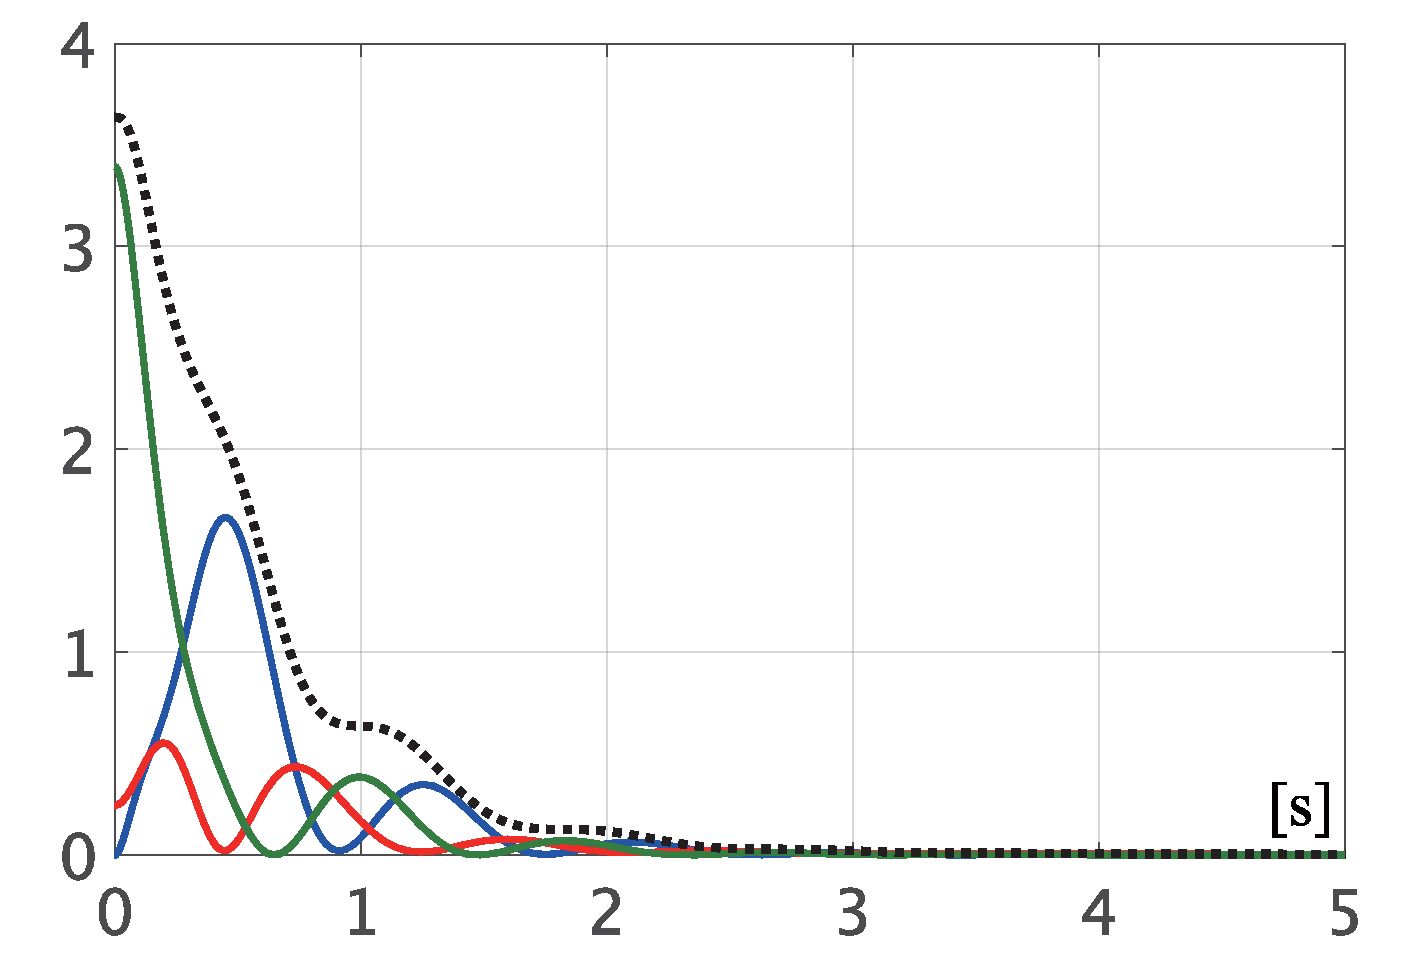
\includegraphics[width = 1.0\linewidth]{figs/Wnlin1}
    \subcaption{Initial value corresponding to steady tidal current state 1}
%    \medskip
  \end{minipage}
  \begin{minipage}{0.49\linewidth}
    \centering
    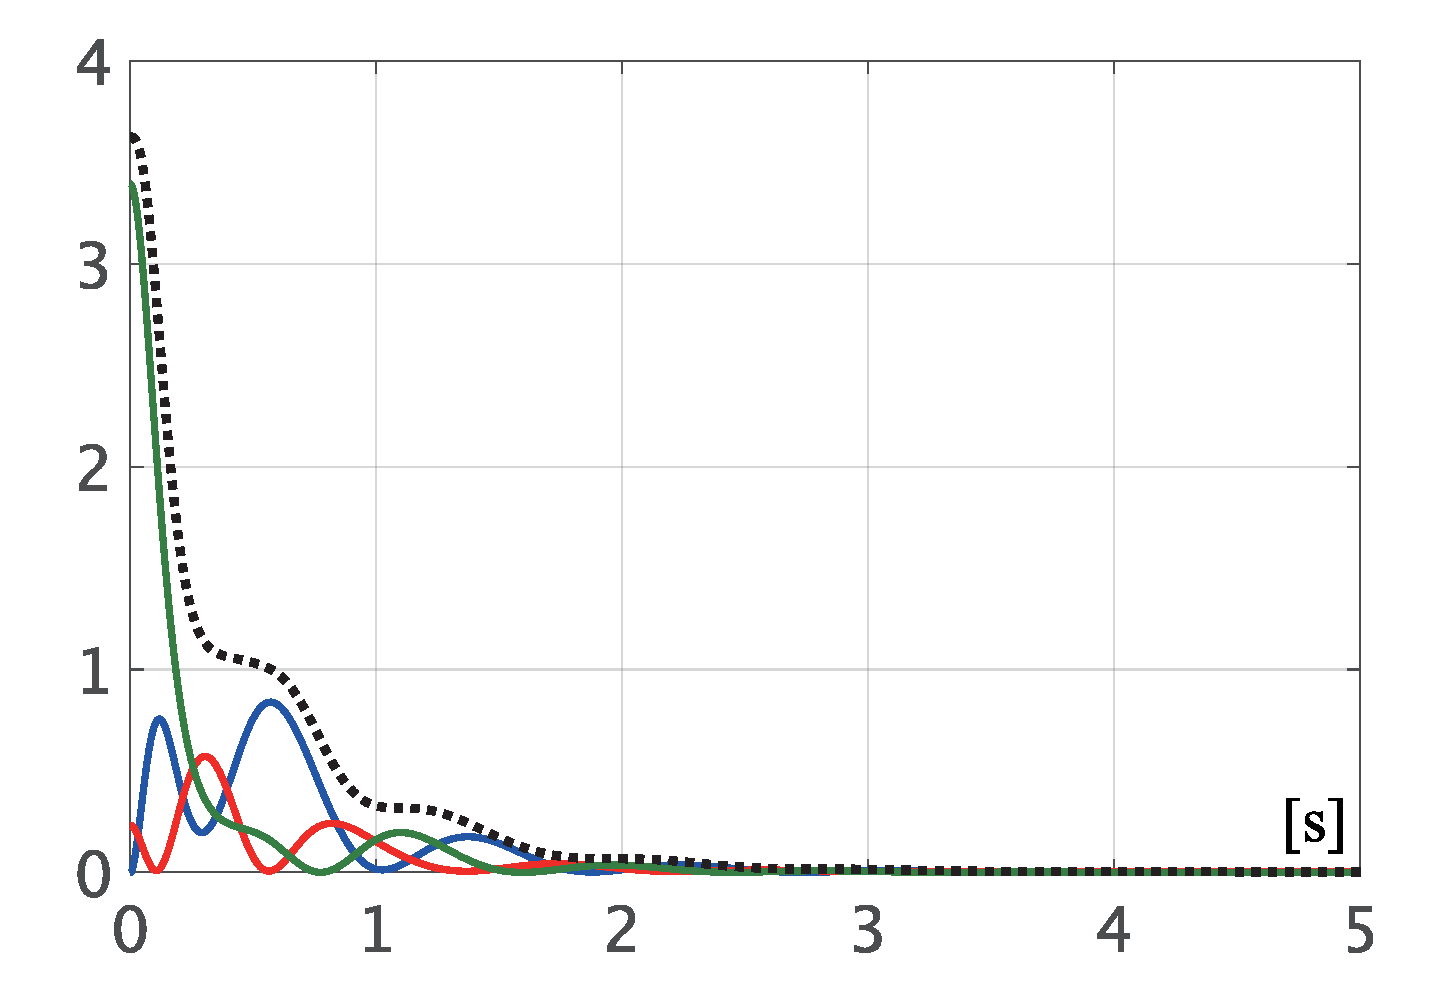
\includegraphics[width = 1.0\linewidth]{figs/Wnlin2}
    \subcaption{Initial value corresponding to steady tidal current state 2}
%    \medskip
  \end{minipage}
  }
  \medskip
  \caption{\textbf{Time variation of the accumulation function with respect to the initial value response}
  \\  \centering(Blue: $W_{x^{\star}_{\mathds{F}}}$, Red:$W_{x^{\star}_{\mathds{G}}}$,
  Green: $W_{\xi^{\star}}$, Black: Total sum)}
  \label{fig:LyapWnlin}
\medskip
\end{figure}



%式(\ref{eq:sys2G})の電気サブシステム$\mathds{G}$の平衡点に依らない受動性を解析する。
%以下では,$\mathds{G}$のすべての時間変数である$(\delta_i, E_i)_{i\in \mathcal{I}_{\rm G}}$と
%$(|\bm{V}_i|, \angle \bm{V}_i)_{i\in \mathcal{I}_{\rm G} \cup \mathcal{I}_{\rm L}}$を並べた列ベクトルを$x_{\mathds{G}}$と表す。
%
%
%なお,ここまでの議論の結果から,式(\ref{eq:connds})における入出力信号はそれらの定常値
%\[
%u_{\mathds{F}}^{\star} =0
%,\qquad
%y_{\mathds{F}}^{\star} =0
%,\qquad
%u_{\mathds{K}}^{\star} =0
%,\qquad
%y_{\mathds{K}}^{\star} =v_{\mathds{F}}^{\star}
%= -y_{\mathds{G}}^{\star}
%,\qquad
%u_{\mathds{G}}^{\star} =0
%\]
%に漸近収束することもわかる。

\smallskip
\subsubsection{The range where the potential energy function is convex}

Below, we show that the condition necessary for the potential energy function $U_{\mathds{G}}(x_{\mathds{G}})$ of Equation \ref{eq:potWx} to be a convex function corresponds to the passive power transmission conditions (i) and (iii) of definition \ref{def:passtrans} discussed in the passive analysis of the linear approximation model.
In the present discussion, the passive power transmission condition (ii) is assumed.

In the setting of the linear approximation model of Section \ref{sec:linpasana}, we consider a situation wherein the generator is connected to all of the bus bars.
In other words, the subscript sets of the generator buses and load bus bars are:

\[
\mathcal{I}_{\rm G} = \{1,\ldots,N\}
,\qquad
\mathcal{I}_{\rm L} = \emptyset
\]
At this time, by applying the Kron reduction of generator buses, the electrical subsystem $\mathds{G}$ of Equation (\ref{eq:sys2G}) and the equivalent ordinary differential equation system can be obtained as:
\begin{align*}%\label{eq:kronGds}
\mathds{G}_i : 
\simode{
\dot{\delta}_i &= u_{\mathds{G}_i}
\\
\taudi \dot{E}_i & = 
 -\tfrac{ \Xsi }{ \Xti }E_i
 - \left(
\Xsi - \Xti
\right)
\sum_{j=1}^{N}
E_j 
B_{ij}^{\rm red}
\sfcos \delta_{ij}
+ V_{{\rm field}i}^{\star}
\\
y_{\mathds{G}_i}&=  -E_i \sum_{j=1}^{N}
 E_j 
B_{ij}^{\rm red}
\sfsin \delta_{ij}
}
\end{align*}
related to $i \in \mathcal{I}_{\rm G}$, where $\delta_{ij}$ expresses $\delta_i -\delta_j$.
When the susceptance matrix of the power grid that summarizes $B_{ij}$ of Equation (\ref{eq:sys2G}), $B$, is being expressed, the reduced susceptance $B_{ij}^{\rm red}$ is defined as the $(i,j)$th element of:
\begin{align}\label{eq:susred}
B^{\rm red}
:= -
\bigl\{
\sfdiag \left( \Xti \right)   
-
\sfdiag \left( \Xti \right) B \sfdiag \left( \Xti \right)
\bigr\}^{-1}
\end{align}
The potential energy function of Equation \ref{eq:potWx} corresponding to the expression of this ordinary differential equation system is:
\begin{align}\label{eq:potWxred}
U_{\mathds{G}}^{\rm red} (z_{\mathds{G}})  := 
 \frac{1}{2} 
\sum_{i=1}^N
\left\{
\frac{ \Xsi E_i^2 }{ \Xti ( \Xsi - \Xti )}  
+ E_i \sum_{j=1}^{N}
 E_j 
B_{ij}^{\rm red}
\sfcos \delta_{ij}
\right\}
\end{align}
where the vector with all $\delta_i$ and $E_i$ is expressed as $z_{\mathds{G}}$.
If we calculate the partial differential related to the internal state, the following is obtained:
\begin{align*}
\frac{\partial U_{\mathds{G}}^{\rm red} }{\partial \delta_i}(z_{\mathds{G}})  = y_{\mathds{G}_i}
,\qquad
\frac{\partial U_{\mathds{G}}^{\rm red} }{\partial E_i} (z_{\mathds{G}}) = 
\frac{V_{{\rm field}i}^{\star} - \taudi\dot{E}_i  }{ \Xsi - \Xti }
\end{align*}
Similarly, the following is true for the steady state:
\begin{align*}
\frac{\partial U_{\mathds{G}}^{\rm red} }{\partial \delta_i} ( z^{\star}_{\mathds{G}} )
= y_{\mathds{G}_i}^{\star}
,\qquad
\frac{\partial U_{\mathds{G}}^{\rm red} }{\partial E_i} ( z^{\star}_{\mathds{G}} ) = 
\frac{V_{{\rm field}i}^{\star}  }{ \Xsi - \Xti }
\end{align*}
Therefore, if we define the corresponding storage function as:
\[ 
W_{z^{\star}_{\mathds{G}}}^{\rm red} (z_{\mathds{G}}) = U_{\mathds{G}}^{\rm red} (z_{\mathds{G}}) 
- U_{\mathds{G}}^{\rm red} (z^{\star}_{\mathds{G}}) 
- \left\{ \nabla U_{\mathds{G}}^{\rm red}(z^{\star}_{\mathds{G}}) \right\}^{\sf T}
 (z_{\mathds{G}}-z^{\star}_{\mathds{G}})
\]
similar to Equation \ref{eq:disineqGds}, its time derivative can be evaluated as:
\[
\frac{d}{dt}W_{z^{\star}_{\mathds{G}}}^{\rm red} \bigl(z_{\mathds{G}}(t) \bigr)
 \leq 
(y_{\mathds{G}}-y_{\mathds{G}}^{\star})^{\sf T} (u_{\mathds{G}}- u_{\mathds{G}}^{\star})
\]
Note that all elements of the contracted susceptance matrix $B^{\rm red}$ in Equation \ref{eq:susred} are nonpositive.
This fact can be shown as follows
From the discussion in the \ref{sec:admathp} clause, the susceptance matrix $B$ is a negative definite matrix with non-diagonal elements that are nonnegative.
Therefore:
\[
B_{-}:= \sfdiag \left( \Xti \right)   
-
\sfdiag \left( \Xti \right) B \sfdiag \left( \Xti \right)
\]
is a positive definite matrix with non-diagonal elements that are nonpositive,\textbf{M-matrix}.
It is known that all the elements of the inverse of the M-matrix are nonnegative \cite{kodama1981system}.
Therefore, all elements of $B^{\rm red}=-B_-^{-1}$ are nonpositive.

\begin{COLUMN}
\noindent \textbf{Hessian matrix}:
A condition necessary for a second-order differentiable function $f:\mathbb{R}^n\rightarrow \mathbb{R}$ to be a convex function over a certain range $\mathcal{X}$ is that the following is positive semi-definite for all $x\in \mathcal{X}$:
\[
\nabla^2 f(x):=
\mat{
\tfrac{\partial^2 f}{\partial x_1^2} (x) & \cdots & \tfrac{\partial^2 f}{\partial x_1 \partial x_n} (x) \\
\vdots & \ddots & \vdots \\
\tfrac{\partial^2 f}{\partial x_n \partial x_1} (x) & \cdots &\tfrac{\partial^2 f}{\partial x_n^2} (x)
}
\]
This matrix is called the \textbf{Hessian matrix} of the function $f$ \cite{boyd2004convex}.
\end{COLUMN}

The fact that the potential energy function $U_{\mathds{G}}^{\rm red} (z_{\mathds{G}})$ of Equation \ref{eq:potWxred} being a convex function is characterized by the fact that the Hessian matrix $\nabla^2 U_{\mathds{G}}^{\rm red} (z_{\mathds{G}})$ is a positive semi-definite matrix.
\begin{align}\label{eq:UGhess}
\nabla^2 U_{\mathds{G}}^{\rm red} (z_{\mathds{G}})
=
\mat{
L(z_{\mathds{G}})  &  - \hat{B}^{\sf T}(z_{\mathds{G}}) \\
- \hat{B}(z_{\mathds{G}}) & -\hat{A}(z_{\mathds{G}})
}
\end{align}
in the $(i,j)$th element.
\begin{align*}
\spliteq{
L_{ij}(z_{\mathds{G}}) & := 
\frac{\partial^2 U_{\mathds{G}}^{\rm red} }{\partial \delta_i \partial \delta_j} (z_{\mathds{G}})
=
\left\{
\begin{array}{cl}
-E_i \sum_{j=1, j\neq i}^{N} E_j B_{ij}^{\rm red} \sfcos(\delta_{ij}), &\quad i=j \\
E_i  E_j B_{ij}^{\rm red} \sfcos(\delta_{ij}), & \quad i\neq j
\end{array}
\right.
  \\
\hat{A}_{ij}(z_{\mathds{G}}) &:=  
- \frac{\partial^2 U_{\mathds{G}}^{\rm red} }{\partial E_i \partial E_j} (z_{\mathds{G}})
=
\left\{
\begin{array}{cl}
-\left(B_{ii}^{\rm red}+\tfrac{ \Xsi }{ \Xti ( \Xsi - \Xti )} \right), &\quad i=j \\
-B_{ij}^{\rm red} \sfcos(\delta_{ij}), & \quad i\neq j
\end{array}
\right. \\
\hat{B}_{ij}(z_{\mathds{G}})  &:= 
- \frac{\partial^2 U_{\mathds{G}}^{\rm red} }{\partial E_i \partial \delta_j} (z_{\mathds{G}})
=
\left\{
\begin{array}{cl}
\sum_{j=1, j\neq i}^{N} E_j B_{ij}^{\rm red} \sfsin(\delta_{ij}), &\quad i=j \\
-E_j B_{ij}^{\rm red} \sfsin(\delta_{ij}), & \quad i\neq j
\end{array}
\right. 
}
\end{align*}
$\nabla^2 U_{\mathds{G}}^{\rm red} (z_{\mathds{G}}^{\star})$, which is an evaluation of the Hessian matrix of Equation \ref{eq:UGhess} with the equilibrium point, is the same as the matrix $P_G$ of Equation \ref{eq:defPG} which appeared in the passivity analysis of the electrical subsystem that was linearly approximated in Section \ref{sec:linpasana}.
The positive semi-definite nature of this $P_G$ guaranteed that the storage function that shows the passivity of the linear approximation model of $\mathds{G}$ is a positive semi-definite function.
As such, a condition necessary for $U_{\mathds{G}}^{\rm red} (z_{\mathds{G}}^{\star})$ to be a convex function is equal to the condition necessary for $P_G$ to be positive semi-definite, which is also equal to the passive power transmission conditions (i) and (iii) holding.

If we consider this along with the result of Section \ref{sec:linmathana}, it is defined as a range where the potential energy function $U_{\mathds{G}}^{\rm red} (z_{\mathds{G}})$ of Equation \ref{eq:potWxred} becomes a convex function:
\[
\mathcal{E}_{\mathds{G}}:=
\left\{
z_{\mathds{G}}^{\star} : \nabla^2 U_{\mathds{G}}^{\rm red} (z_{\mathds{G}}^{\star}) 
\succeq 0
\right\}
\]
however, it is also the “maximum” equilibrium point set that is able to present frequency stability based on passivity.
The reason for this is, as was shown in Section \ref{sec:nesconana}, is that the passive power transmission conditions are conditions necessary for an electrical subsystem that was linearly approximated near a specific equilibrium point to be passive.
In other words, at an equilibrium point $z_{\mathds{G}}^{\star}$, where $\nabla^2 U_{\mathds{G}}^{\rm red} (z_{\mathds{G}}^{\star}) $ is not positive semi-definite, the electrical subsystem $\mathds{G}$ does not become passive.

In contrast, if the initial value $z_{\mathds{G}}(0)$ of the electrical subsystem is set near the equilibrium point $z_{\mathds{G}}^{\star}$ belonging to the set $\mathcal{E}_{\mathds{G}}$,
for all combinations of physical parameters $(M_,D_i,\taudi)_{i \in \mathcal{I}_{\rm G}}$,
the entire feedback control system asymptotically converges to a steady power flow distribution where supply and demand are balanced.

\section{Transient stabilization control}\label{sec:transcont}

\subsection{Decentralized control of generators with excitation system}

In an electrical power system, when discussing the stable range size for an equilibrium point and the level of stability, the term \textbf{transient stability} is often used.
In this Section, we provide an outline of the mathematical model and the properties of the \textbf{excitation system} implemented to improve the transient stability of an electrical power system.
The excitation system is a localized controller that is usually installed “individually” to each generator.
It locally measures the voltage phasor and current phasor of the bus bar to which the generator is connected, and the internal state of the generator, to control by automatically adjusting the field voltage. The main element of the excitation system is a control equipment called an \textbf{automatic voltage regulator (AVR)} that maintains the desired bus bar voltage. Furthermore, an additional control algorithm, called a \textbf{power system stabilizer (PSS)} might be incorporated to control the disturbance caused by the AVR.
From Section \ref{sec:avrov} to Section \ref{sec:pssov}, we explain the standard models and control effects.

%\[
%\tau_{{\rm d}} \dot{E}  = 
% - \left\{ \tfrac{X_{{\rm d}}}{X_{{\rm d}}'}E
%-\left(
%\tfrac{X_{{\rm d}i}}{X_{{\rm d}i}'}-1
%\right)
%|\bm{V}_i| \sfcos (\delta_i - \angle \bm{V}_i ) 
%\right\}
%+ V_{{\rm field}i}
%\]
%
%\[
%\taudi \dot{E}_i  = 
% - E_i
%-(
%X_{{\rm d}i} - X_{{\rm d}i}'
%)
%|\bm{I}_i| \sfsin (\delta_i - \angle \bm{I}_i ) 
%+ V_{{\rm field}i}
%\]
%
%




\subsection{Standard AVR model}\label{sec:avrov}

There are many standardized AVR models.
For example, a report on standardization by the IEEE \cite{ieee2016ieee} lists more than 40 types of standard models.
AVR models are roughly divided into DC, AC, and Static models.
Below, we discuss typical DC and static models.


First, let us talk about the \textbf{IEEE Type DC1 excitation system model}, which is an AVR DC model.
Please see \cite[Section 7.9.2]{anderson2008power} and \cite[Section 8.6.3]{kundur1994power} for the model details.
Here, we discuss AVR of generators connected to the bus bar $i$, but for the sake of simplification, we omit subscripts $i$.
Specifically, we use the generator model discussed in Section \ref{sec:genfund}:
\begin{align}\label{eq:gendifavr}
\simode{
\dot{\delta}&= \omega_0  \Delta \omega\\
M   \Delta \dot{\omega}&= 
 - D \Delta\omega  
 - P
+P_{{\rm mech}}
\\
\taud \dot{E} & = 
- \Ifd 
+ V_{{\rm field}}
}
\end{align}
For the purpose of discussion, we defined: which is equivalent to the value of the field current of generators with the unit system of pu.
\begin{align}\label{eq:efield}
\Ifd := \frac{ \Xs }{ \Xt }E
-\left(
\frac{ \Xs }{ \Xt }-1
\right)
|\bm{V}| \sfcos (\delta - \angle \bm{V} )
\end{align}
The active power and reactive power output by generators are:
%\begin{align*}
%\spliteq{
%P & =  \frac{E |\bm{V} |}{ \Xt } \sfsin(\delta -  \angle \bm{V}), \\
%Q & =  \frac{E |\bm{V} |}{ \Xt } \sfcos (\delta - \angle \bm{V}) - \frac{|\bm{V}|^2}{ \Xt }
%}
%\end{align*}
\[
P  =  \frac{E |\bm{V} |}{ \Xt } \sfsin(\delta -  \angle \bm{V}), \qquad
Q  =  \frac{E |\bm{V} |}{ \Xt } \sfcos (\delta - \angle \bm{V}) - \frac{|\bm{V}|^2}{ \Xt }
\]
In a case involving a salient pole generator model discussed in Section \ref{sec:genmodadv}, $\Ifd$ is defined by substituting $\Xt$ and $\Xs$ of Equation \ref{eq:efield} with $X_{{\rm d}}'$,$X_{\rm d}$.

As shown in \FIGref{fig:avrdc1}, the IEEE Type DC1 excitation system model is a regulator that inputs the absolute value $|\bm{V}|$ of the bus bar voltage phasor and outputs the field voltage $V_{\rm field}$ of generators.
However, as supplementary input signals, reference signal $V_{\rm ref}^{\star}$ that adjusts the absolute value of bus bar voltage phasor to the desired value and control signal $V_{\rm pss}$ output by PSS are added.
The IEEE Type DC1 excitation system model of AVR consists of four basic types of equipment — \textbf{voltage transformer}, \textbf{comparator}, \textbf{amplifier}, and \textbf{exciter} — as well as a supplementary \textbf{stabilizing circuit}.
Below, we explain the dynamic characteristics of each.


\begin{figure}[t]
\centering
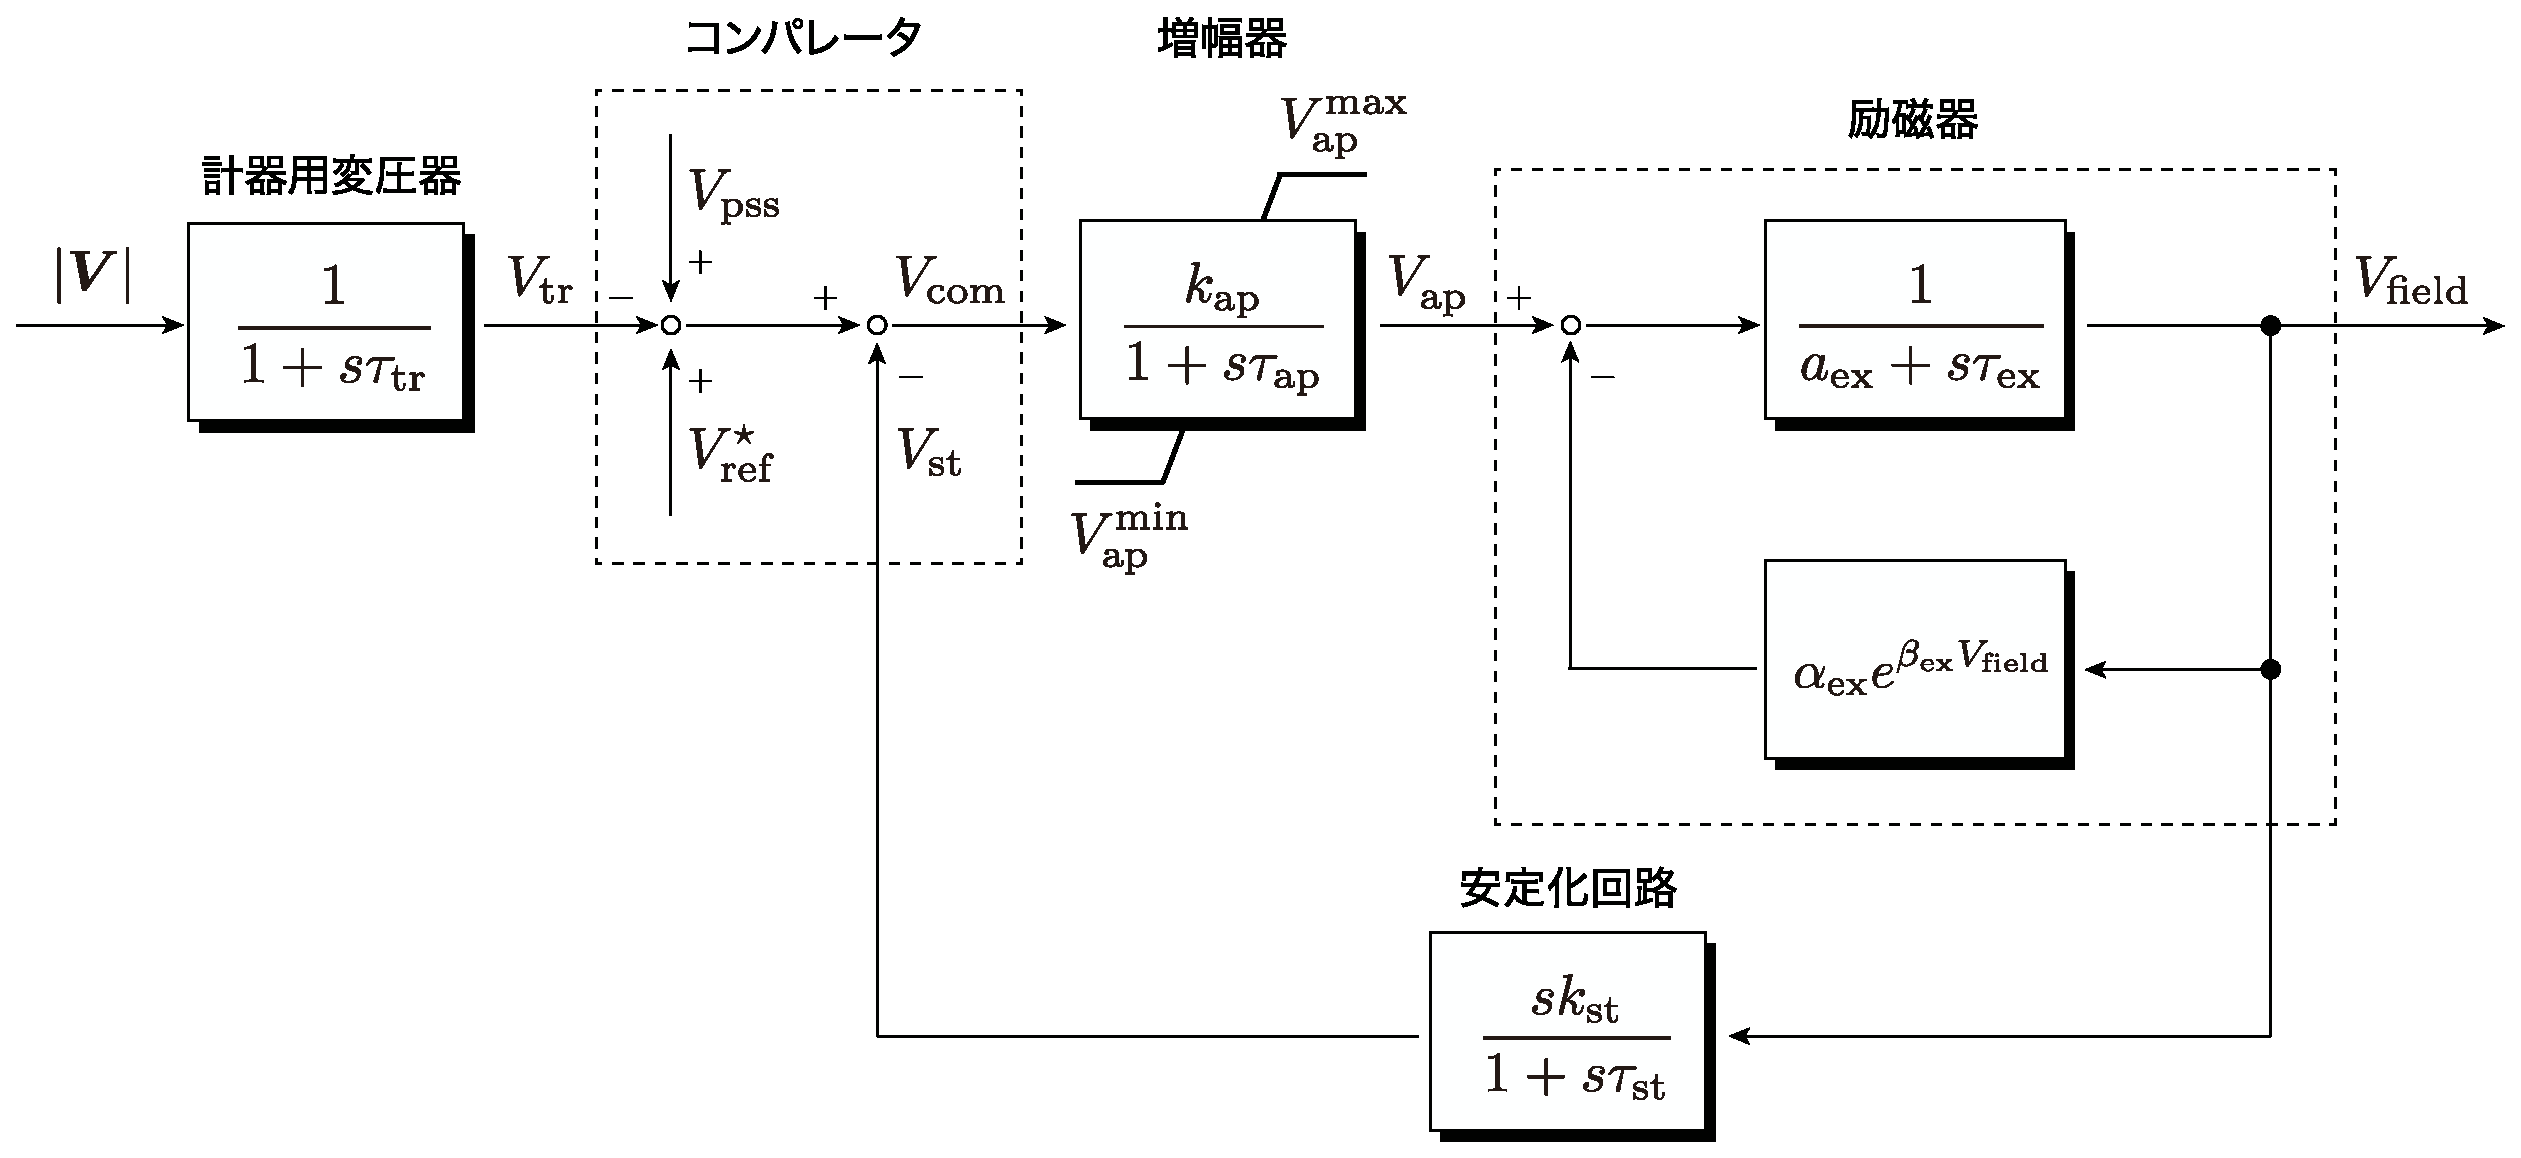
\includegraphics[width = 0.99\linewidth]{figs/avrdc1}
\medskip
\caption{\textbf{IEEE DC1 type model of automatic voltage regulator}}
\label{fig:avrdc1}
\medskip
\end{figure}


\smallskip
\subsubsection{Voltage transformer}

\begin{subequations}\label{eq:stanAVR}
This is a piece of equipment that lowers the bus bar voltage to a usable voltage for the control circuit, and its dynamic characteristic is modelled as a first-order lag filter:
\begin{align}\label{eq:trnsmod}
\tau_{\rm tr} \dot{V}_{\rm tr} = - V_{\rm tr} +  |\bm{V}|
\end{align}
Generally, the time constant $\tau_{\rm tr}$ is sufficiently small; thus, an output $V_{\rm tr}$ of the voltage transformer is almost the same as the absolute value $|\bm{V}|$ of the bus bar voltage phasor.

\smallskip
\subsubsection{Comparator}

This is a piece of equipment that outputs the difference between the voltage transformer output $V_{\rm tr}$ and the reference signal $V_{\rm ref}^{\star}$.
PSS output $V_{\rm pss}$ discussed below is added as a signal that adjusts a constant, $V_{\rm ref}^{\star}$.
In addition, if a stabilizing circuit of the excitation system is to be incorporated, its output $V_{\rm st}$ is also fed back.
In other words, the comparator is modelled as:
\begin{align}\label{eq:compmod}
V_{\rm com} = V_{\rm ref}^{\star} + V_{\rm pss}- V_{\rm tr}
- V_{\rm st}
\end{align}
As discussed, since $V_{\rm tr}$ is almost the same as $|\bm{V}|$, if PSS output $V_{\rm pss}$ and the stabilizing circuit output $V_{\rm tr}$ are 0, the comparator output $V_{\rm com}$ is almost the same as the difference between the reference signal and the absolute value of the bus bar voltage phasor $V_{\rm ref}^{\star} - |\bm{V}|$

\smallskip
\subsubsection{Amplifier}

This is a piece of equipment to drive the exciter by multiplying the output of the comparator $V_{\rm com}$. There are many types such as rotary and electromagnetic types, but in most cases, it is modelled as:
\begin{align}\label{eq:ampmod}
\tau_{\rm ap} \dot{V}_{\rm ap}=
\left\{
\begin{array}{cl}
- V_{\rm ap} + k_{\rm ap} V_{\rm com}, & \mbox{$V_{\rm ap}^{\rm min} < V_{\rm ap} < V_{\rm ap}^{\rm max}$ ~or~ $V_{\rm ap} V_{\rm com}\leq 0$ } \\
0, & \mbox{otherwise}
\end{array}
\right.
\end{align}
%\begin{align}\label{eq:ampmod}
%\tau_{\rm ap} \dot{V}_{\rm ap}=
%\left\{
%\begin{array}{cl}
%0, & V_{\rm ap}\in \{ V_{\rm ap}^{\rm min},V_{\rm ap}^{\rm max} \},\ V_{\rm ap}V_{\rm com}>0\\
%- V_{\rm ap} + k_{\rm ap} V_{\rm com}, & \mbox{otherwise}
%\end{array}
%\right.
%\end{align}
%\begin{align}\label{eq:ampmod}
%\simode{
%\tau_{\rm ap} \dot{V}_{\rm ap} & = - V_{\rm ap} + k_{\rm ap} V_{\rm com} \\
%V_{\rm ap}^{\rm sat} & = \sfsat(V_{\rm ap};V_{\rm ap}^{\rm min},V_{\rm ap}^{\rm max})
%}
%\end{align}
Time constant $\tau_{\rm ap}$ and gain $k_{\rm ap}$ are non-negative constants, and saturation that limits the internal state $V_{\rm ap}$ within the range of $[V_{\rm ap}^{\rm min},V_{\rm ap}^{\rm max}]$ is expressed by conditional branching. 
Saturation might be set for output instead of the internal state.
In a transient state relative to large disturbances, such as ground faults, the range of the upper and lower limits of saturation might be set to be large \cite[Section 4.3]{sauer2017power}.

\smallskip
\subsubsection{Exciter}

This is a piece of equipment that generates field voltage from the amplifier output $V_{\rm ap}^{\rm sat}$, and is modelled as a nonlinear first-order system:
\begin{align}\label{eq:extmod}
\tau_{\rm ex}\dot{V}_{\rm field} =
- \Bigl( 
a_{\rm ex} + 
\underbrace{\alpha_{\rm ex} e^{\beta_{\rm ex} V_{\rm field}}}_{\ast} 
\Bigr) V_{\rm field}
+V_{\rm ap}
\end{align}
Though $\tau_{\rm ex}$ is a positive constant, the sign of $a_{\rm ex}$ varies between papers.
In addition, the term expressed with “$\ast$” is nonlinear because of the impact of magnetic saturation in the exciter, and $\alpha_{\rm ex}$ and $\beta_{\rm ex}$ are both non-negative.
Each constant is set so that dynamic characteristic of the exciter is stable near the usual operating point.

\smallskip
\subsubsection{Stabilizing circuit}

This is a supplementary circuit installed to improve the stability of the excitation system.
In the IEEE Type DC1 excitation system model, it is expressed as a feedback mechanism of the differential value of the field voltage; in other words, its dynamic characteristic is expressed as:
\begin{align}\label{eq:stcmod}
\tau_{\rm st}\dot{V}_{\rm st} =
- V_{\rm st}
+ k_{\rm st} \dot{V}_{\rm field}
\end{align}
The time constant $\tau_{\rm st}$ and gain $k_{\rm st}$ are non-negative This output of the stabilizing circuit $V_{\rm st}$ is fed back to the comparator of Equation \ref{eq:compmod}.
\end{subequations}

The IEEE Type DC1 excitation system model of AVR is a combination of Equation \ref{eq:trnsmod} to Equation \ref{eq:stcmod} discussed above.
The reference values of each parameter are summarized in \ref{table:AVRpara1} and \ref{table:AVRpara2}.
The unit of the time constant is [s] while other units are [pu].


\begin{table}[h]
\medskip
 \caption{\textbf{Parameter example of IEEE DC1 type model}}
 \label{table:AVRpara1}
 \centering
  \begin{tabular}{lcccccc}
   \hline
 &  $\tau_{\rm tr}$ & $\tau_{\rm ap}$ & $k_{\rm ap}$ & $V_{\rm ap}^{\rm max}$ & $V_{\rm ap}^{\rm min}$ \\
   \hline \hline
   例1 \cite[Table D.3. Unit F2]{anderson2008power}& 0.00 & 0.05 & 57.1 & 1.00 & $-1.00$\\
   例2 \cite[Table 7.3]{sauer2017power}& 0.00 & 0.2 & 20 & $\infty$ & $-\infty$\\
%   例2 \cite[8.6.3節]{kundur1994power}& 0.05 & 0.89 & 187 & 1.70 & $ -1.70 $\\
   \hline
  \end{tabular}
\end{table}

\begin{table}[h]
\medskip
 \caption{\textbf{Parameter example of IEEE DC1 type model (continued)}}
 \label{table:AVRpara2}
 \centering
  \begin{tabular}{lccccccc}
   \hline
&    $\tau_{\rm ex}$ & $a_{\rm ex}$ & $\alpha_{\rm ex}$ & $\beta_{\rm ex}$ & $\tau_{\rm st}$ & $k_{\rm st}$\\
   \hline \hline
  例1 \cite[Table D.3. Unit F2]{anderson2008power}& 0.50 & $-0.045$ & 0.0012 & 1.21 & 1.00 & 0.08\\
   例2 \cite[Table 7.3]{sauer2017power}& 0.314 & $1.0$ & 0.0039 & 1.555 & 0.35 & 0.063 \\
%  例2 \cite[8.6.3節]{kundur1994power}& 1.15 & $-0.30$ & 0.014 & 1.55 & 0.62 & 0.058 \\
   \hline 
  \end{tabular}
\end{table}


%\begin{table}[h]
%\medskip
% \caption{計器用変圧器と増幅器のパラメータ範囲(参考値)}
% \label{table:AVRpara1}
% \centering
%  \begin{tabular}{|c|c|c|c|c|c|}
%   \hline
%   $\tau_{\rm tr}$ & $\tau_{\rm ap}$ & $k_{\rm ap}$ & $V_{\rm ap}^{\rm max}$ & $V_{\rm ap}^{\rm min}$ \\
%   \hline \hline
%   0 -- 0.06 & 0.02 -- 0.25 & 25 -- 400 & 1.0 -- 8.2 & $V_{\rm ap}^{\rm max} \times (-1)$\\
%   \hline
%  \end{tabular}
%\end{table}
%
%\begin{table}[h]
%\medskip
% \caption{励磁器と安定化回路のパラメータ範囲(参考値)}
% \label{table:AVRpara2}
% \centering
%  \begin{tabular}{|c|c|c|c|c|c|}
%   \hline
%    $\tau_{\rm ex}$ & $a_{\rm ex}$ & $\alpha_{\rm ex}$ & $\beta_{\rm ex}$ & $\tau_{\rm st}$ & $k_{\rm st}$\\
%   \hline \hline
%   0.5 -- 1.3 & $-0.17$ -- $-0.05$ & 0.0016 -- 0.011 & 0.79 -- 1.56 & 0.35 -- 1.0 & 0.01 -- 0.08\\
%   \hline
%  \end{tabular}
%\end{table}

\begin{figure}[t]
\centering
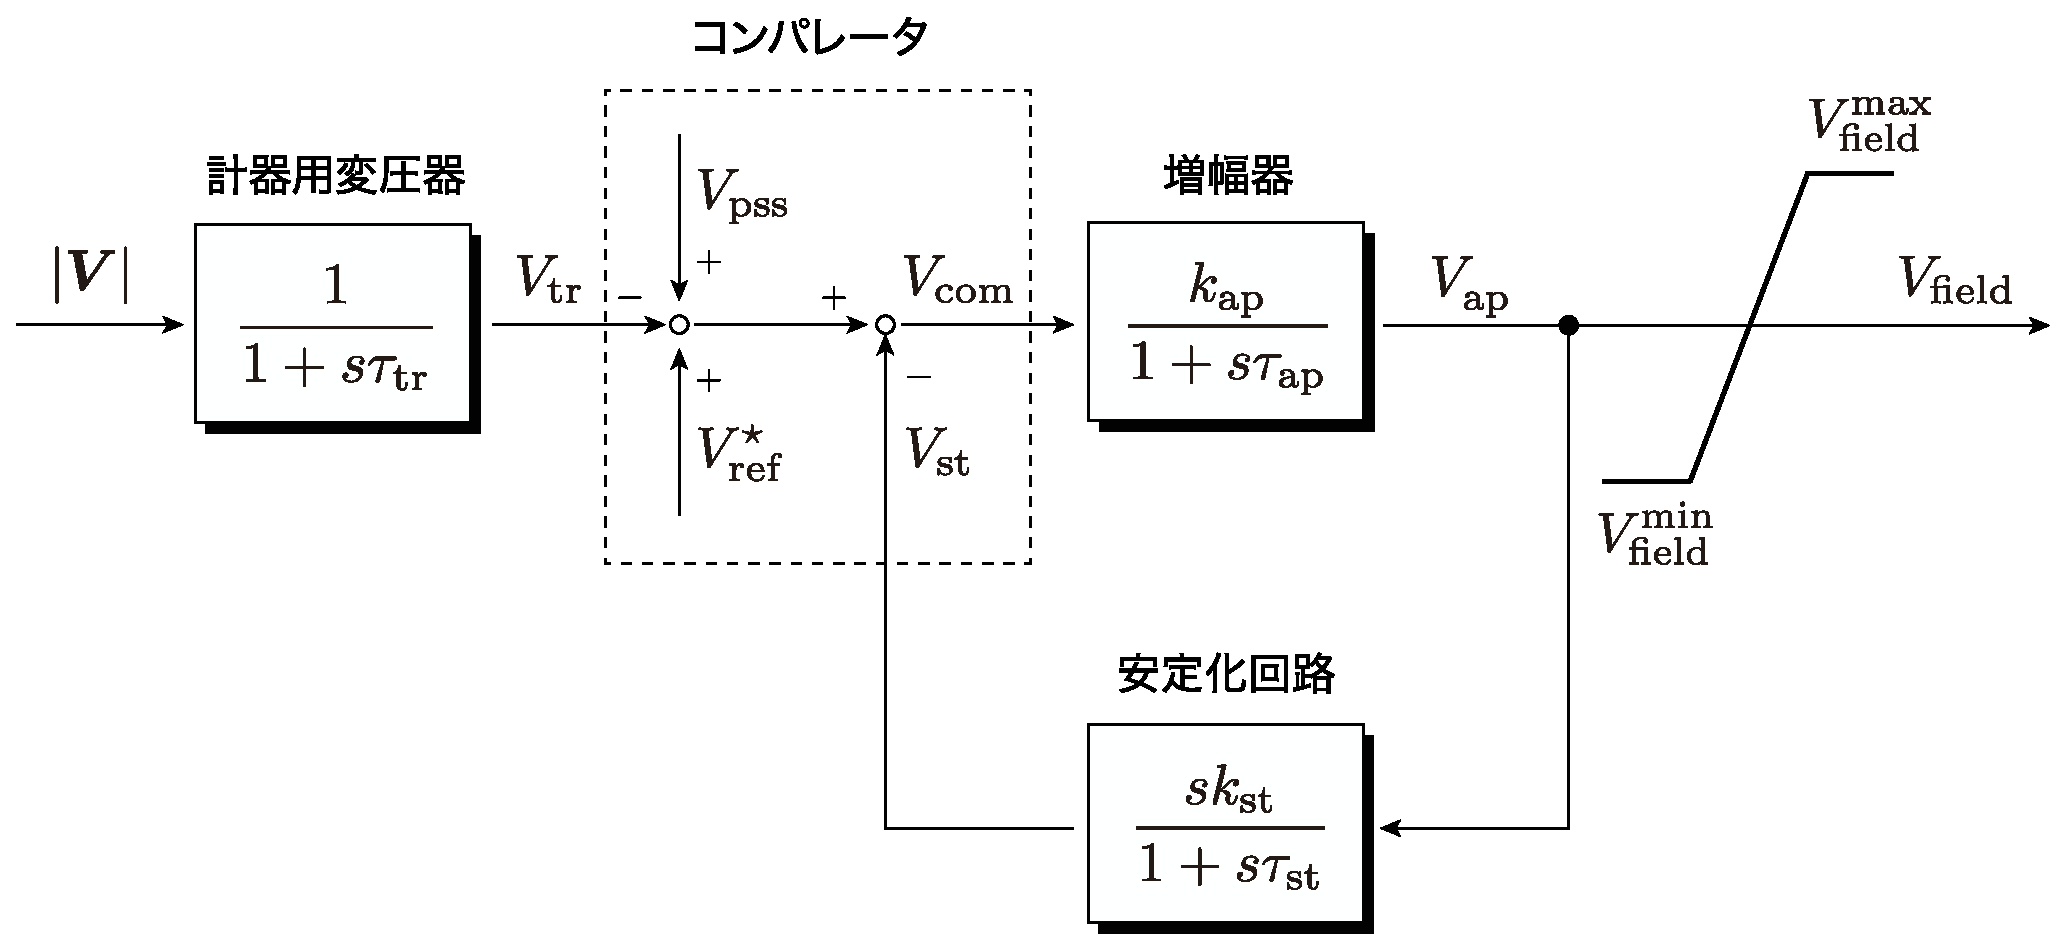
\includegraphics[width = .85\linewidth]{figs/avrst1}
\medskip
\caption{\textbf{IEEE ST1 type model of automatic voltage regulator}}
\label{fig:avrst1}
\medskip
\end{figure}

Next, let us talk about the \textbf{IEEE Type ST1 excitation system model}, which is a static model with a faster response, although its structure is the same as the IEEE Type DC1 excitation system model.
With this AVR model, the exciter model of Equation \ref{eq:extmod} is expressed as a static relationship with a sufficiently small time constant for the exciter:
\[
V_{\rm field} = \sfsat \bigl( V_{\rm ap};V_{\rm field}^{\rm min},V_{\rm field}^{\rm max} \bigr)
\]
%\[
%V_{\rm field} = 
%\left\{
%\begin{array}{cl}
%V_{\rm field}^{\rm min}, & V_{\rm ap} \leq V_{\rm field}^{\rm min} \\
%V_{\rm ap}, & V_{\rm field}^{\rm min} < V_{\rm ap} \leq V_{\rm field}^{\rm max} \\
%V_{\rm field}^{\rm max}, & V_{\rm ap} > V_{\rm field}^{\rm max}
%\end{array}
%\right.
%\]
$\sfsat$ is a saturation constant of output and is defined by:
\[
\sfsat(x;\underline{\alpha},\overline{\alpha}) := \left\{
\begin{array}{cl}
\underline{\alpha}, & x \leq \underline{\alpha} \\
x, & \underline{\alpha} < x \leq \overline{\alpha} \\
\overline{\alpha}, & x> \overline{\alpha}
\end{array}
\right.
\]
The upper and lower limits of the output saturation are modelled to be dependent on the absolute value of the bus bar voltage phasor \cite[Section 8.3]{kundur1994power}.
Specifically, this is expressed as:
\[
V_{\rm field}^{\rm min} = \gamma_{-} |\bm{V}|, \qquad
V_{\rm field}^{\rm max} = \gamma_{+} |\bm{V}|
-
k_0 \Ifd
\]
using $\Ifd$ of Equation \ref{eq:gendifavr} in addition to $|\bm{V}|$, where $\gamma_{-}$,$\gamma_{+}$,$k_{0}$ is a non-negative constant.
\FIGref{fig:avrst1} shows the block diagram of this model.
Since $|\bm{V}|$ becomes 0 during the ground fault of bus bars, field voltage $V_{\rm field}$ is not output because of AVR.

Since the response speed of the exciter is sufficiently fast in the IEEE Type ST1 Excitation System Model, the stabilizing circuit is often unnecessary.
When time constant $\tau_{\rm ap}$ of the amplifier is sufficiently small, and its dynamic characteristic can be ignored: 
\begin{align}\label{eq:avrst1}
\simode{
\tau_{\rm tr} \dot{V}_{\rm tr} & = - V_{\rm tr} +  |\bm{V}|  \\
V_{\rm ap} &= k_{\rm ap} ( V_{\rm ref}^{\star} + V_{\rm pss}- V_{\rm tr} )\\
V_{\rm field} & = \sfsat \left(
V_{\rm ap};
V_{\rm field}^{\rm min},V_{\rm field}^{\rm max} 
\right)
}
\end{align}
is used as the simplified first-order model.
For example, this model is used in \cite[Section 12.4]{kundur1994power} and \cite[Section 4.2.2]{pal2006robust}.
Parameter examples are shown in the Examples 1 and 2 in \ref{table:AVRparast1}.

\begin{table}[h]
\medskip
 \caption{\textbf{IEEE ST1 type model parameter example}}
 \label{table:AVRparast1}
 \centering
  \begin{tabular}{lccccccccc}
   \hline
 &  $\tau_{\rm tr}$ & $\tau_{\rm ap}$ & $k_{\rm ap}$ & $\gamma_{+}$ & $\gamma_{-}$ & $k_{0}$ & $\tau_{\rm st}$ & $k_{\rm st}$\\
   \hline \hline
   Example 1 \cite[Section 8.6.3]{kundur1994power}& 0.015 & 0 & 200 & 7.00 & $-6.40$ & 0.04 & 0 & 0\\
   Example 2 \cite[Table H.23]{ieee2016ieee}& 0.02 & 0 & 210 & 6.43 & $-6.00$ & 0.038 & 0 & 0 \\
   Example 3 \cite[Section V]{chow2004power}& 0 & 0.076 & 36.66 & $\infty$ & $-\infty$ & 0 & 0 & 0 \\
   Example 4 \cite[Table 4]{sadamoto2019dynamic}& 0 & 0.05 & 20 & $\infty$ & $-\infty$ & 0 & 0 & 0 \\
   \hline
  \end{tabular}
\end{table}

Though the time constant $\tau_{\rm ap}$ of the amplifier is not 0, models with the time constant $\tau_{\rm tr}$ of the voltage transformer being 0 and models without output saturation are sometimes used.
In such a case, it can be expressed as:
\begin{align}\label{eq:avrst1s}
\simode{
\tau_{\rm ap} \dot{V}_{\rm ap}&=
- V_{\rm ap} + k_{\rm ap} (V_{\rm ref}^{\star} + V_{\rm pss}- |\bm{V}|)\\
{V}_{\rm field}&=V_{\rm ap}
}
\end{align}
Parameter examples of this model are shown in Examples 3 and 4 in \ref{table:AVRparast1}.

The value of the reference signal $V_{{\rm ref}}^{\star}$ in Equations \ref{eq:avrst1} and \ref{eq:avrst1s} is determined as:
\begin{align}\label{eq:avrref}
V_{{\rm ref}}^{\star} = \frac{V_{{\rm field}}^{\star}}{k_{{\rm ap}}}+|\bm{V}^{\star}|
\end{align}
when the steady value $V_{{\rm field}}^{\star}$ of the desired field voltage and the steady value $|\bm{V}^{\star}|$ of the absolute value for the bus bar voltage are given, in a real system operation, the steady values of the bus bar voltage and field voltage are unknown values that change by load distribution and so on;
thus, the value of the reference signal $V_{{\rm ref}}^{\star}$ is specified by using the value of the standard bus bar voltage and field voltage.

\subsection{Control effect of AVR}

Let us analyze the control effect of AVR using a simple electrical power system model.

\begin{例}[自動電圧調整器による定態安定性と過渡安定度の変化]\label{ex:avreffect}
Let us consider an electrical power system model consisting of three bus bars discussed in the Examples \ref{ex:derY}, \ref{ex:pf3bus} and \ref{ex:inires}.
The physical constants of generators and transmission lines are set to the same value as the Example \ref{ex:inires}.
In addition, loads connected to bus bar 2 are set to the constant impedance model, and the values from the first row of \ref{table:loadpara1} are used as impedance.
AVR is set to the IEEE Type ST1 Excitation System Model of Equation \ref{eq:avrst1}. AVR incorporated into generator 1 and generator 3 is the same, and values from Example 1 in \ref{table:AVRparast1} are used as parameters.

First, let us confirm the change in the set of the steady power flow distribution (stable equilibrium point) that is statically stable against AVR.
Specifically, the steady value of the interval voltage of generators, $E_1^{\star}$ and $E_3^{\star}$, are fixed to the values in the rightmost column of \ref{table:genst13a}, and the difference of the steady value of the rotor argument, $\delta_3^{\star}-\delta_1^{\star}$, is changed as a parameter.
In this manner, the small signal stability of the steady power flow distribution in a corresponding electrical power system is determined based on approximate linearization.

Without losing generality, $\delta_1^{\star}$ or $\delta_3^{\star}$ can be set to 0.
If the steady value of the internal state of each generator is determined, the steady value of the corresponding mechanical torque and field voltage can be determined by:
\begin{align*}
\simode{
P_{{\rm mech}i}^{\star} &= %\textstyle
  f_i \left( \delta^{\star},E^{\star} \right)
\\
V_{{\rm field}i}^{\star} & = %\textstyle
   \tfrac{ \Xsi }{\Xti }  E_i^{\star}  - \left(
\Xsi - \Xti
\right)
g_i \left( \delta^{\star},E^{\star} \right)
}
\qquad
 i \in \{1,3\}
\end{align*}
$\delta^{\star}$ and $E^{\star}$ are vectors with $\delta_i^{\star}$ and $E_i^{\star}$, and functions $f_i$ and $g_i$ are defined by Equation \ref{eq:figidef}.
Furthermore, the steady value of the generator bus voltage phasor can be obtained as:
\begin{align*}
\mat{
\bm{V}_1^{\star}\\
\bm{V}_3^{\star}
} =
\left(
\mat{
\tfrac{1}{\bm{j} \Xt_1 } & 0\\
0 & \tfrac{1}{\bm{j} \Xt_3 }
} + 
\bm{Y}_{\rm Kron}
\right)^{-1}
\mat{
\tfrac{e^{\bm{j} \delta_1^{\star}}}{\bm{j} \Xt_1 } & 0 \\
0 & \tfrac{e^{\bm{j} \delta_3^{\star}}}{\bm{j} \Xt_3 }
}
\mat{
E_1^{\star}  \\
E_3^{\star} 
}
\end{align*}
by using Equation \ref{eq:colVi}.
$\bm{Y}_{\rm Kron}$ is the admittance matrix where the load bus bar defined by \ref{eq:Kron} is Kron reduced.
The value of the reference signal $V_{{\rm ref}i}^{\star}$ is determined by Equation \ref{eq:avrref}.

\begin{table}[h]
\medskip
 \caption{\textbf{Steady value of rotor declination that stabilizes the state} 
 \\ \centering(AVR: automatic voltage regulator, PSS: system stabilizer)}
 \label{table:stableeqs}
 \centering
  \begin{tabular}{ccccccccccc}
   \hline
 & (i) Without AVR & (ii) With AVR & (iii) With AVR and PSS \\
   \hline \hline
 $\delta_3^{\star}-\delta_1^{\star}$ Upper limit~[rad]  & $1.03$ & $0.87$ & $1.32$ \\
 $\delta_3^{\star}-\delta_1^{\star}$ Lower limit~[rad] & $-0.90$ & $-0.30$ & $-1.10$  \\
   \hline
  \end{tabular}
\end{table}

\begin{COLUMN}
\noindent \textbf{$\mathcal{L}_2$ norm}:
$\mathcal{L}_2$ norm of function $y:[0,\infty) \rightarrow \mathbb{R}^n$ is
expressed as:
\[
\|y\|_{\mathcal{L}_2} := \sqrt{
\int^{\infty}_{0}
\| y(\tau)\|^2  d \tau
}
\]
と定義される。
この値は,時変な信号のエネルギーを表すものとして解釈できる。
一般に,時刻の経過にしたがって振幅が減衰する信号でない限り,$\mathcal{L}_2$ノルムの値は無限大となる。
なお,``$\mathcal{L}$"の文字は,ルベーグ積分の理論で知られるアンリ・ルベーグ(Henri Lebesgue)の名前に由来する。
\end{COLUMN}

Next, let us confirm an increase in the transient stability by AVR.
Specifically, we perform the following analysis.
First, as a statically stable steady power flow distribution regardless of AVR, we consider where the steady value of the rotor argument difference $\delta_3^{\star}-\delta_1^{\star}$ is $-\tfrac{\pi}{6}$~[rad].
However, the steady value of internal voltage is set to the above value.
Next, the initial value of the electrical power system is changed as a parameter, and $\|\Delta\omega\|_{\mathcal{L}_2}$ is calculated for the obtained time response of the frequency deviation.
$\Delta \omega$ is a vector with $\Delta \omega_1$ and $\Delta \omega_3$.
Similarly, $\||\bm{V}|-|\bm{V}^{\star}| \|_{\mathcal{L}_2}$ is calculated for the time response of the bus bar voltage phasor.
$|\bm{V}|$ is a vector with $|\bm{V}_1|$ and $|\bm{V}_3|$, while $|\bm{V}^{\star}|$ is a vector with $|\bm{V}_1^{\star}|$ and $|\bm{V}_3^{\star}|$.


\FIGref{fig:transientL2} shows the result of the transient stability analysis.
The horizontal axis shows the initial value of the set $\delta_3-\delta_1$, while the vertical axis shows values of $\mathcal{L}_2$ norms for frequency deviation and bus bar voltage phasor deviation generated to the set initial value.
The solid blue line shows a case corresponding to \ref{table:stableeqs}(i) without AVR, and the broken black line shows the case corresponding to (ii) with AVR.
These are plotted in the range of initial values where values of $\mathcal{L}_2$ are finite.
The initial values of the internal voltage $E_1$,$E_3$ are set to the same values as their steady values $E_1^{\star}$,$E_3^{\star}$.
The initial values of frequency deviations $\Delta \omega_1$ and $\Delta \omega_3$ are both set to 0.
From this result, we can see that the transient stability of the frequency deviation and bus bar voltage phasor is improved by AVR.
We can also see that the stable range is somewhat narrowed by AVR.

As a reference, \FIGref{fig:avrsmalld} and \FIGref{fig:avrlarged} show the time response of frequency deviations when the initial value of $\delta_3-\delta_1$ is set to $-1$ and $-\tfrac{\pi}{2}$: (a) is without AVR and (b) is with AVR.
The result shows that by incorporating AVR, the low frequency component of frequency deviation oscillation (central value of oscillation) tends to converge to 0 faster.
On the other hand, regardless of AVR, the attenuation rate of the high frequency component of oscillation does not change notably.
\end{例}



%\begin{figure}[t]
%\centering
%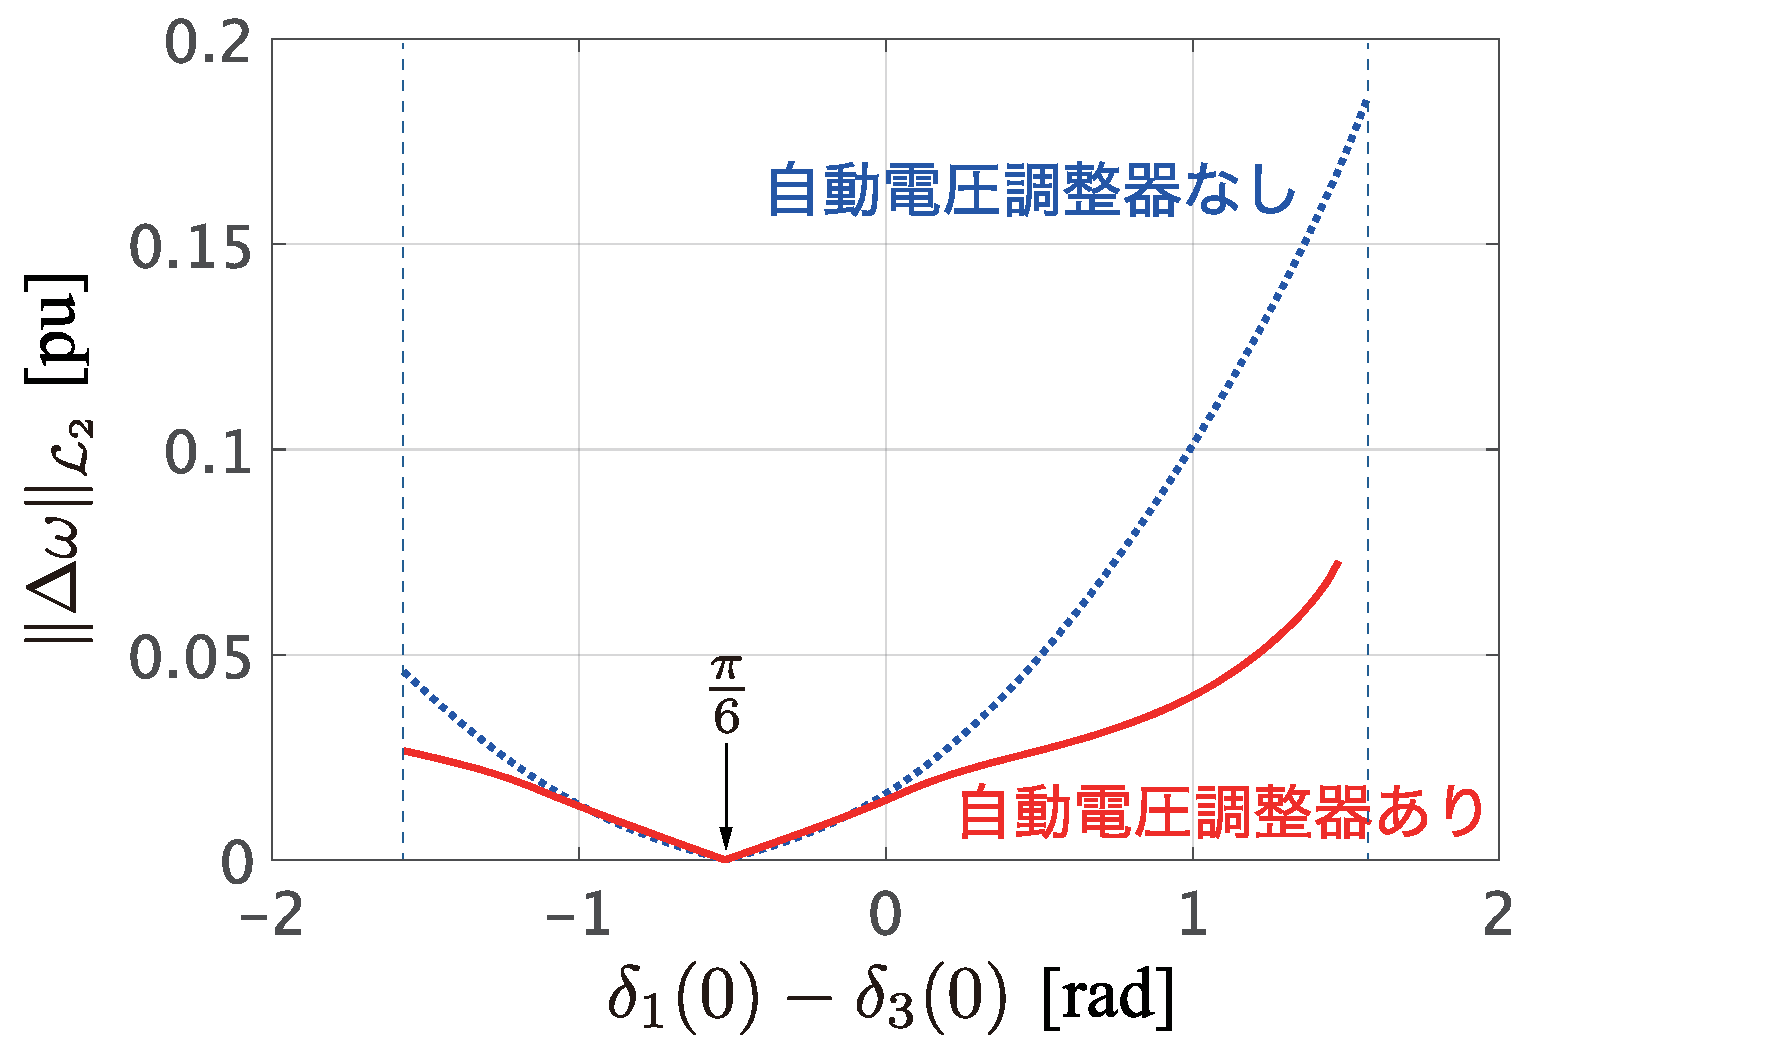
\includegraphics[width = .65\linewidth]{figs/transientL2}
%\medskip
%\caption{\textbf{ 自動電圧調整器による過渡安定度の変化} }
%\label{fig:transientL2}
%\medskip
%\end{figure}

\begin{figure}[t]
  \centering
  {
  \begin{minipage}{0.49\linewidth}
    \centering
    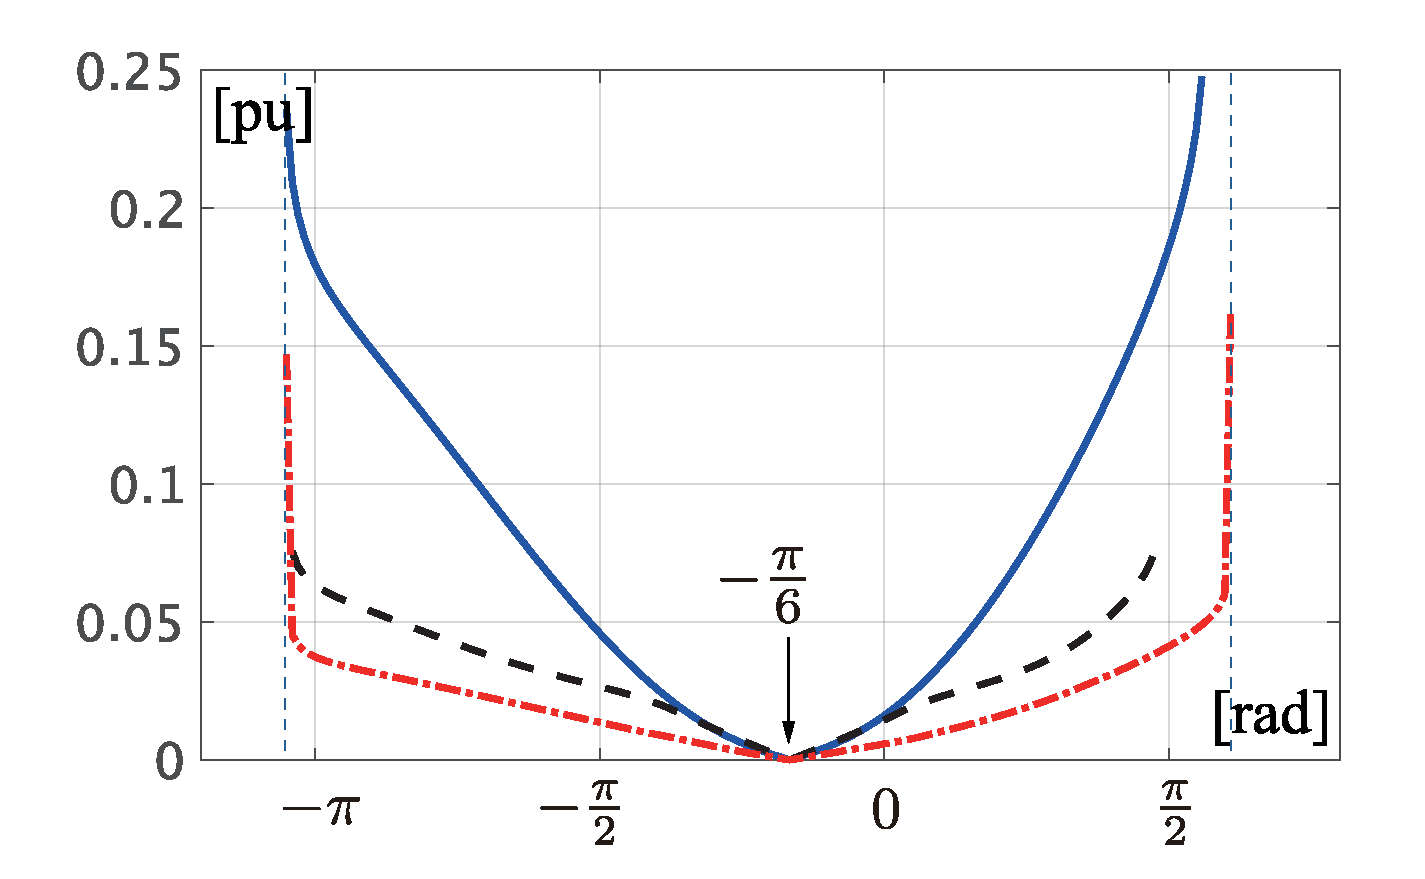
\includegraphics[width = 1.0\linewidth]{figs/transientL2w}
    \subcaption{ $\|\Delta\omega\|_{\mathcal{L}_2}$ }
  \end{minipage}
  \begin{minipage}{0.49\linewidth}
    \centering
    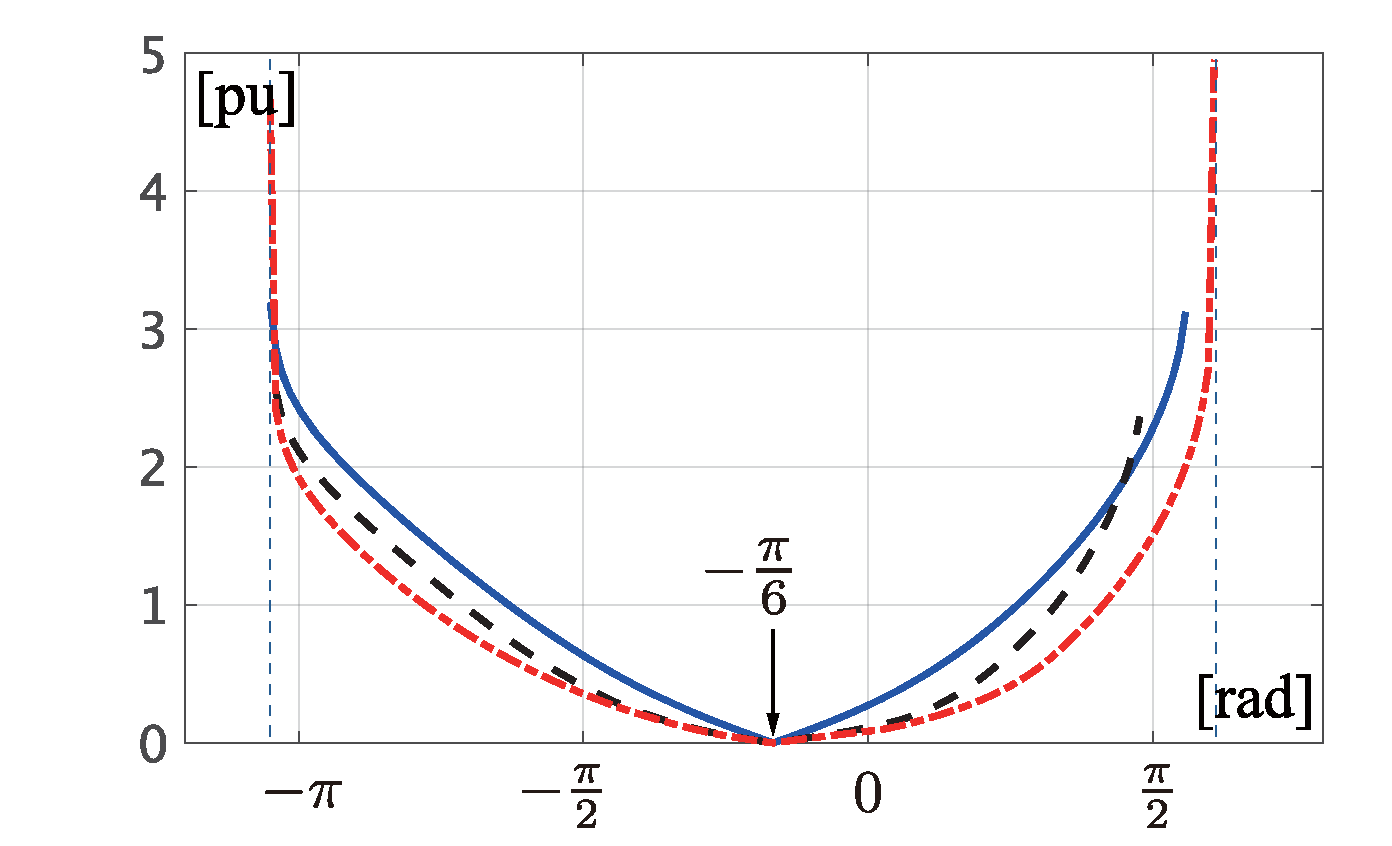
\includegraphics[width = 1.0\linewidth]{figs/transientL2V}
    \subcaption{ $\bigl\||\bm{V}|-|\bm{V}^{\star}| \bigr\|_{\mathcal{L}_2}$}
  \end{minipage}
  \medskip
  \caption{\textbf{Transient stability evaluation for the initial value of the rotor declination difference} 
  \\ \centering(Blue solid line: (i), Black dashed line: (ii), Red chain line: (iii))}
  \label{fig:transientL2}
  }
\medskip
\end{figure}



\begin{figure}[t]
  \centering
  {
  \begin{minipage}{0.49\linewidth}
    \centering
    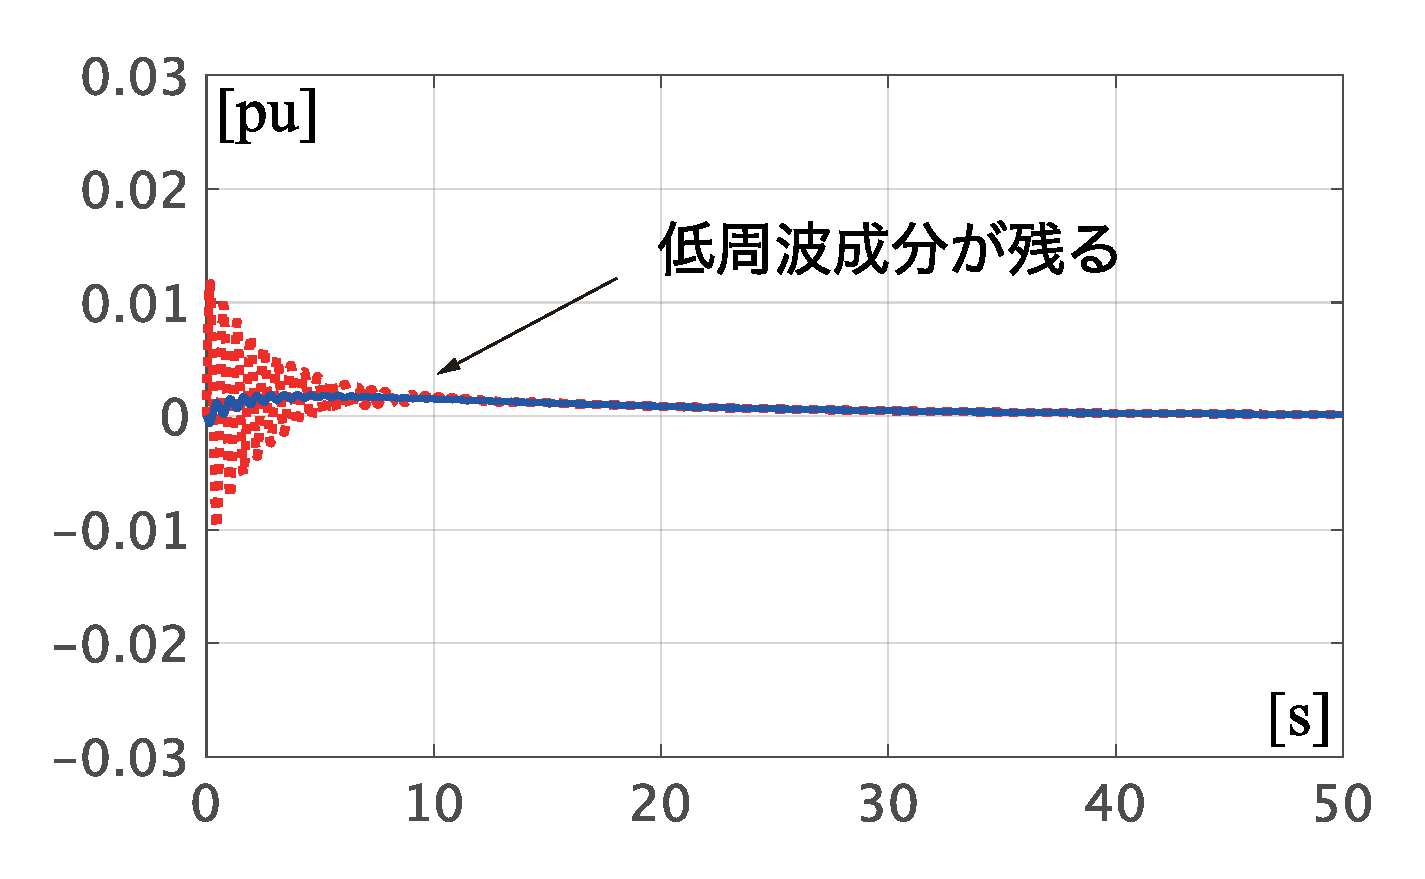
\includegraphics[width = 1.0\linewidth]{figs/woAVRsmall}
    \subcaption{Without AVR}
  \end{minipage}
  \begin{minipage}{0.49\linewidth}
    \centering
    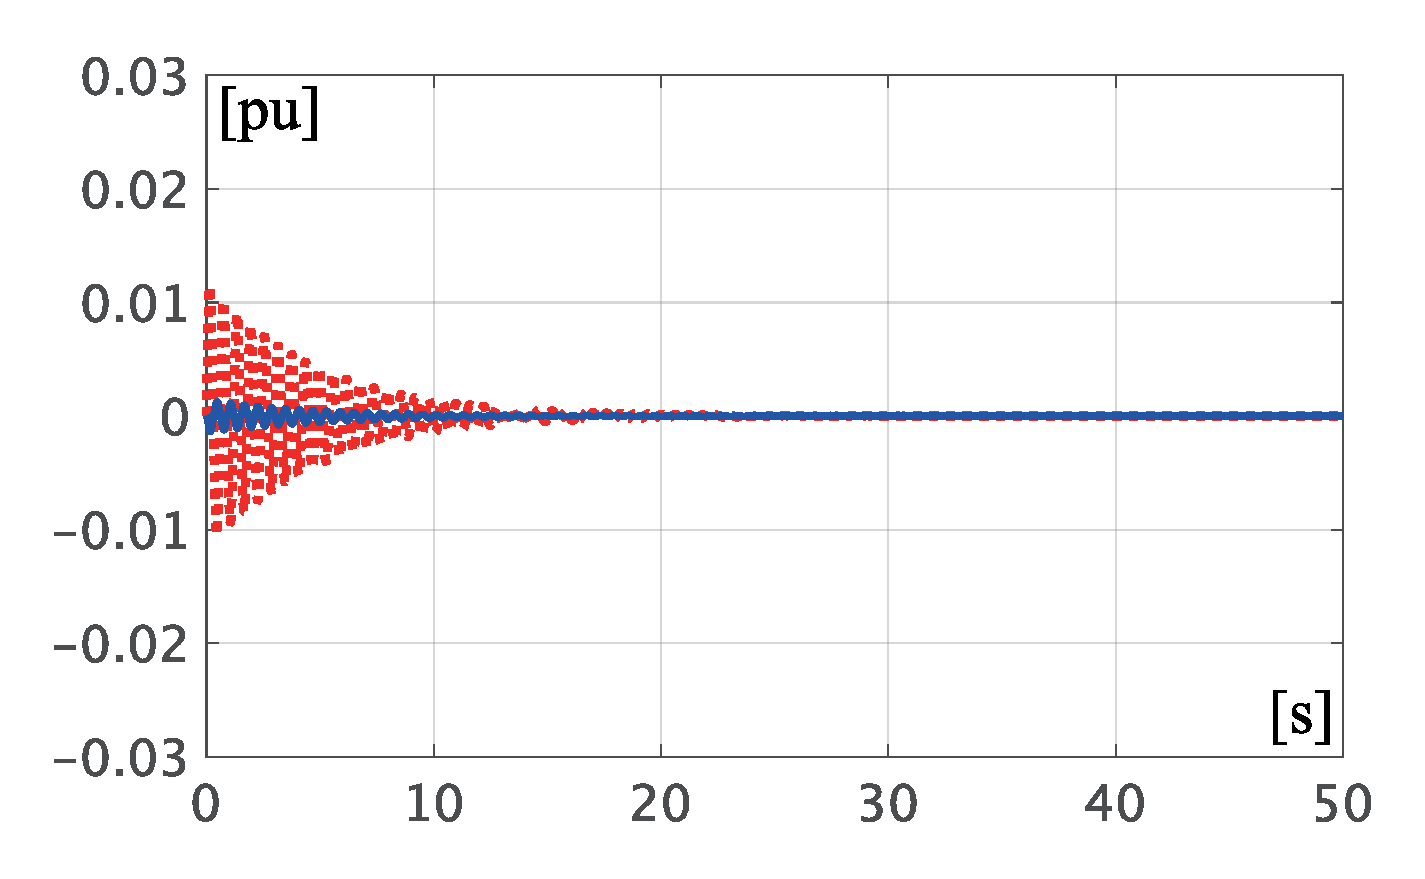
\includegraphics[width = 1.0\linewidth]{figs/wAVRsmall}
    \subcaption{With AVR}
  \end{minipage}
  \medskip
  \caption{\textbf{Initial value response of angular frequency deviation}
  \\ \centering{(Blue solid line: $\Delta\omega_1$, red dashed line: $\Delta\omega_3$)}
  }
  \label{fig:avrsmalld}
  }
\medskip
\end{figure}

\begin{figure}[t]
  \centering
  {
  \begin{minipage}{0.49\linewidth}
    \centering
    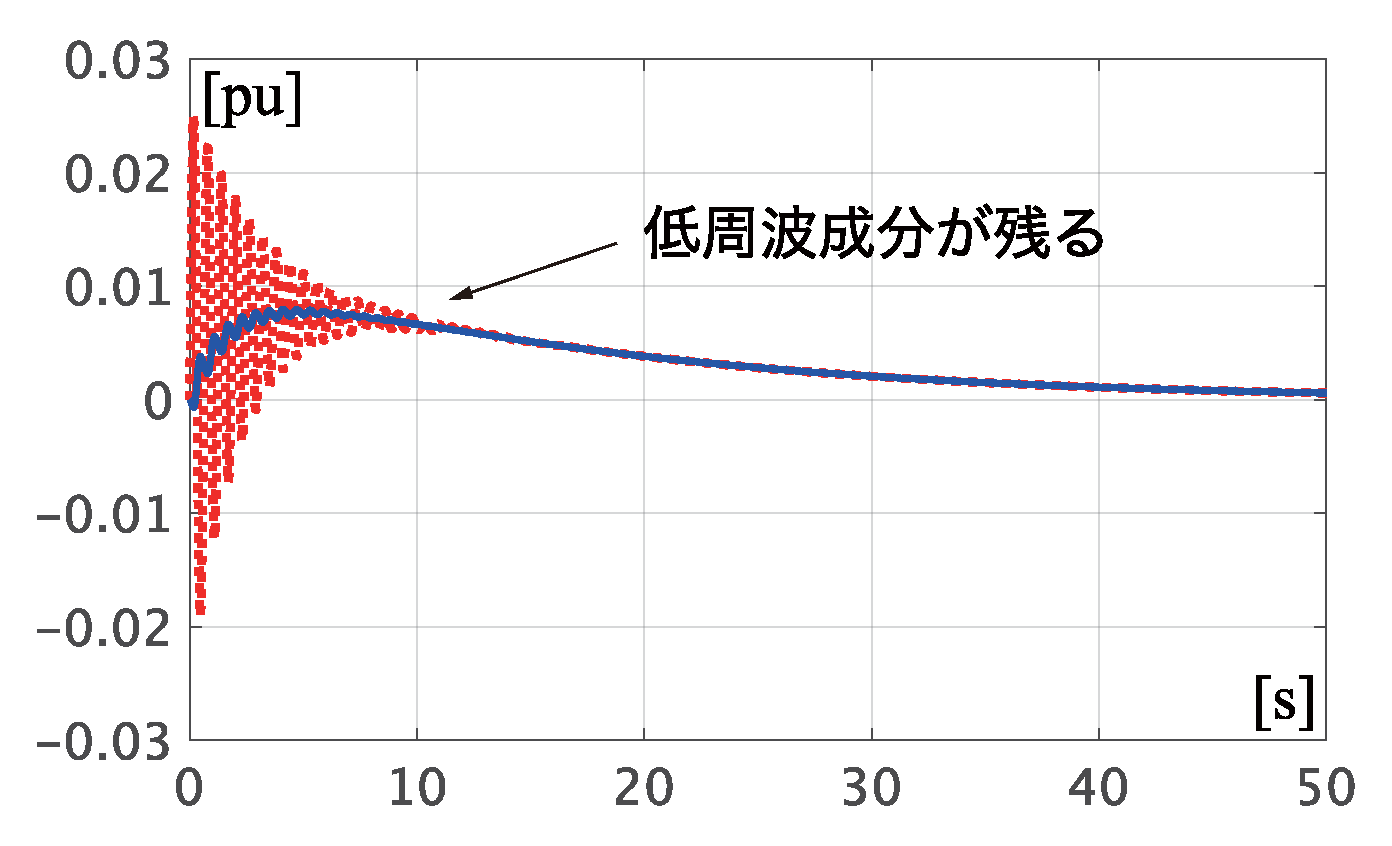
\includegraphics[width = 1.0\linewidth]{figs/woAVRlarge}
    \subcaption{Without AVR}
  \end{minipage}
  \begin{minipage}{0.49\linewidth}
    \centering
    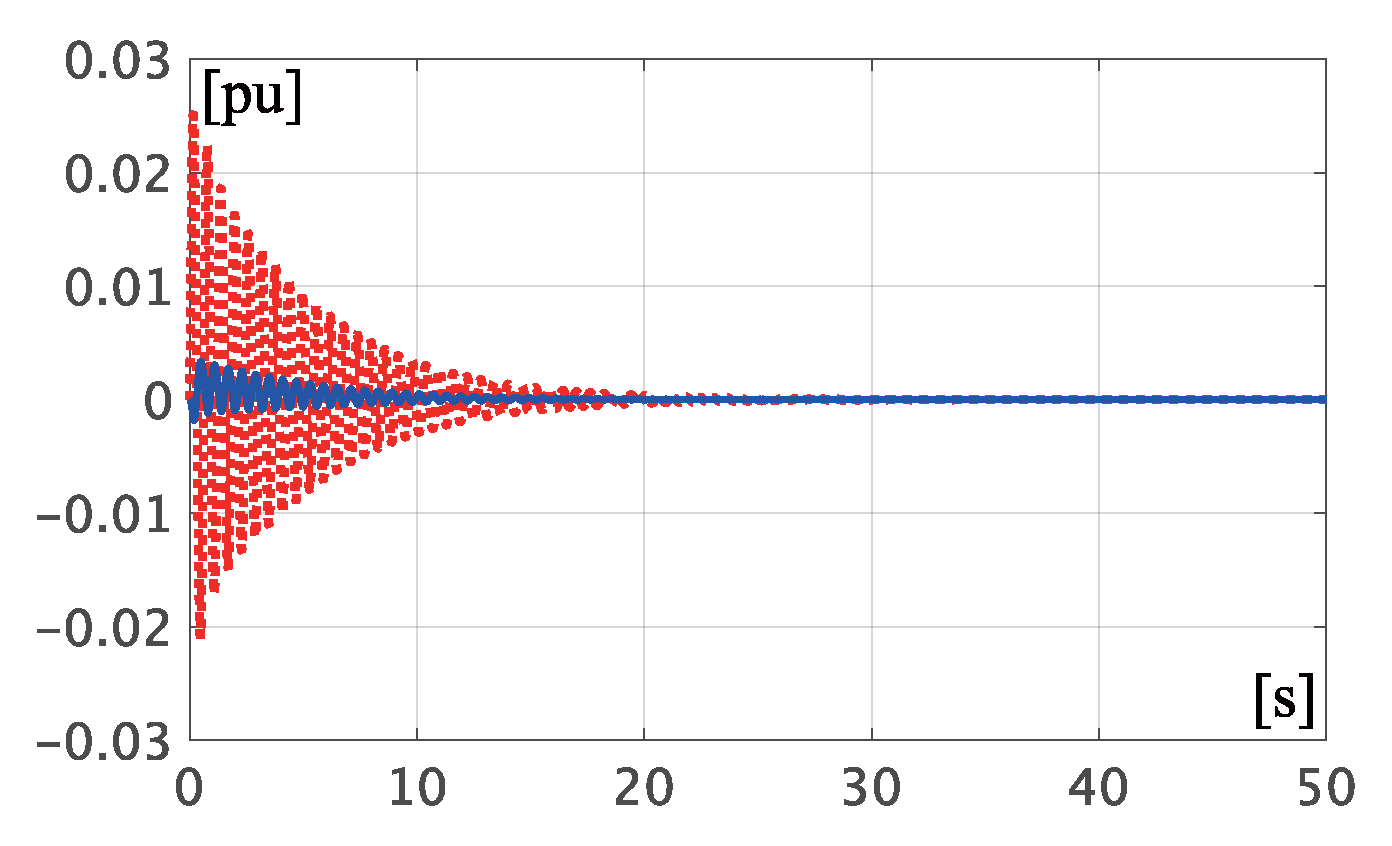
\includegraphics[width = 1.0\linewidth]{figs/wAVRlarge}
    \subcaption{With AVR}
  \end{minipage}
  \medskip
  \caption{\textbf{Initial value response of angular frequency deviation}
  \\ \centering{(Blue solid line: $\Delta\omega_1$, Red dashed line: $\Delta\omega_3$)} 
}
  \label{fig:avrlarged}
  }
\medskip
\end{figure}

The Example \ref{ex:avreffect} shows that while part of the equilibrium point that was stable before becomes unstable by incorporating AVR, the low frequency component of the frequency deviation oscillation is suppressed.
In this sense, the transient stability of the electrical power system improves.
PSS, as explained in the next Section, has a suppressing effect on the high frequency component of oscillation which could not be controlled by AVR.

\subsection{PSS}\label{sec:pssintro}

PSS is a piece of equipment that outputs additional control signal $V_{\rm pss}$ shown in \FIGref{fig:avrdc1} and \FIGref{fig:avrst1}.
Generally, the frequency deviation, active power, and bus bar voltage phasor are calculated for generators to feedback to PSS.
Below, we explain a typical PSS model called the \textbf{IEEE Type PSS1 power system stabilizer model} \cite[Section 9.2]{ieee2016ieee}.
This model mainly consists of a \textbf{washout filter} and \textbf{phase-lead compensator}.
\FIGref{fig:pss1} shows the block diagram. 

\begin{figure}[t]
\centering
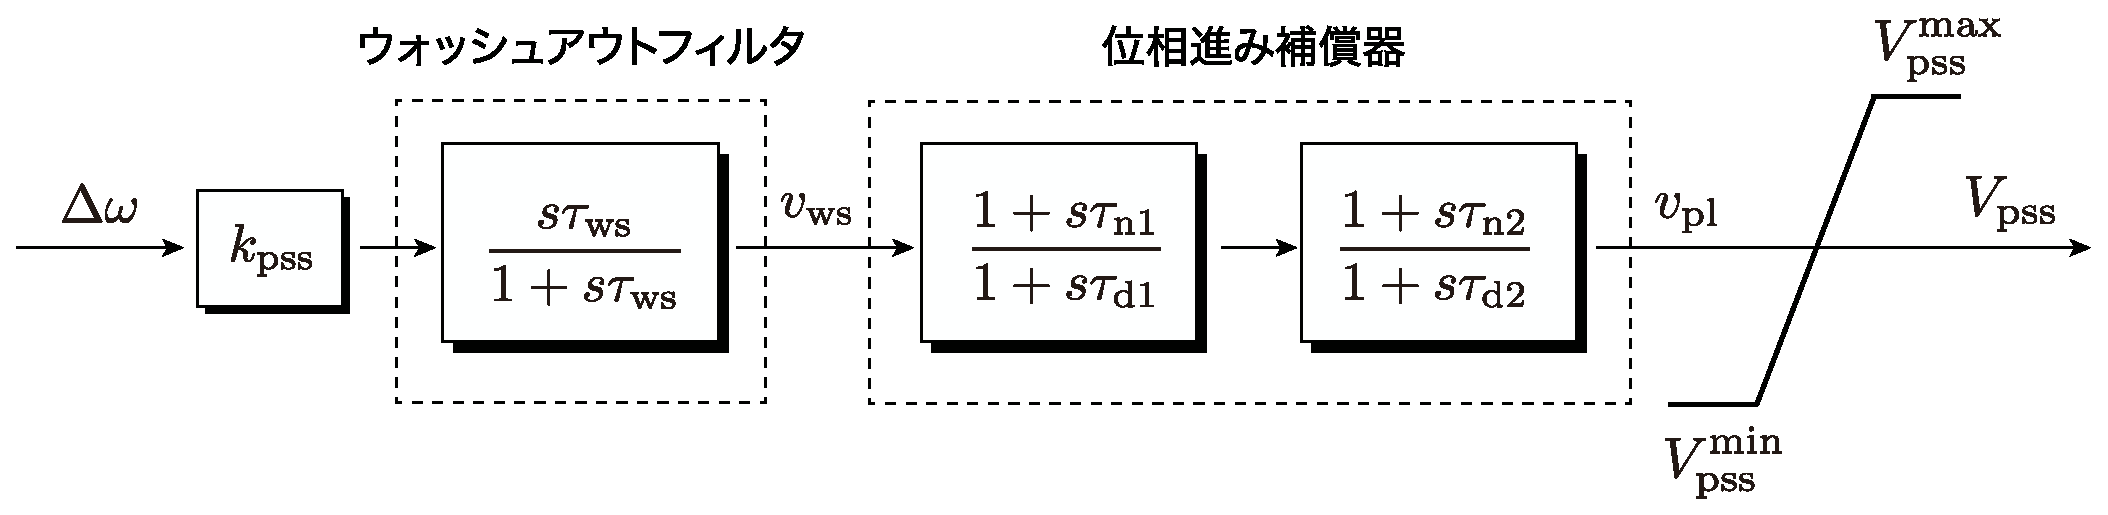
\includegraphics[width = .99\linewidth]{figs/pss1}
\medskip
\caption{\textbf{IEEE PSS1 type model of system stabilizer}}
\label{fig:pss1}
\medskip
\end{figure}


\smallskip
\subsubsection{Washout filter}


It is a high-pass filter to make the steady gain of PSS 0, and its dynamic characteristic is expressed as the following with the frequency deviation $\Delta \omega$ of a generator that has been constant factored by gain $k_{\rm pss}$ as the input: 
\begin{subequations}\label{eq:pss1mod}
\begin{align}\label{eq:washmod}
\simode{
\tau_{\rm ws} \dot{\xi}_{\rm ws} &=
- \xi_{\rm ws}
+ k_{\rm pss} \Delta \omega \\
v_{\rm ws} &= k_{\rm pss} \Delta \omega - \xi_{\rm ws}
}
\end{align}
Clearly, if $\Delta \omega$ is a constant, the output of washout filter $v_{\rm ws}^{\star}$ under a steady state becomes 0.
The role of this filter is to identify the frequency deviation of the electrical power system under a transient state.
Therefore, the time constant $\tau_{\rm ws}$ is often set in a range of 1 to 20 [s] considering the settling time for frequency deviation.


\smallskip
\subsubsection{Phase-lead compensator}
This is a compensator incorporated to alleviate a phase lag from the bus bar voltage phasor to the active power of generators.
To achieve the desired phase lead, one to two phase-lead compensators are often connected in a series.
Specifically, with the washout filter output $v_{\rm ws}$ as the input, its dynamic characteristic is expressed by:

\begin{align}\label{eq:phldmod}
\simode{
\tau_{{\rm d}1} \dot{\xi}_{1} &=
- \xi_{1}
+ \left( 
1- \tfrac{\tau_{{\rm d}1}}{\tau_{{\rm n}1}}
\right)
v_{\rm ws} \\
v_{1} &= \tfrac{\tau_{{\rm n}1}}{\tau_{{\rm d}1}} (v_{\rm ws} - \xi_{1} )
}
\qquad
\simode{
\tau_{{\rm d}2} \dot{\xi}_{2} &=
- \xi_{2}
+ \left( 
1- \tfrac{\tau_{{\rm d}2}}{\tau_{{\rm n}2}}
\right)
v_{1} \\
v_{\rm pl} &= \tfrac{\tau_{{\rm n}2}}{\tau_{{\rm d}2}} (v_{1} - \xi_{2} )
}
\end{align}
%ただし,時定数は$\tau_{{\rm d}1} \leq \tau_{{\rm n}1}$,$\tau_{{\rm d}2} \leq \tau_{{\rm n}2}$となるように設定される。
Finally, the phase-lead compensator output $v_{\rm pl}$ is applied to a saturation function:
\begin{align}\label{eq:psssat}
V_{\rm pss} = \sfsat \left(
v_{\rm pl};
V_{\rm pss}^{\rm min},V_{\rm pss}^{\rm max} 
\right)
\end{align}
\end{subequations}
to obtain the PSS output.
\ref{table:psspara} shows parameter examples of this model.
However, PSS parameters must be determined by considering various elements, such as the dynamic characteristic of each generator, the dynamic characteristic of AVR, load distribution, and power grid properties.
Thus, depending on the illustrated parameter setting, the desired system stability might not be achieved.
In addition, the standard parameter design guidelines of PSS are often based on the single machine infinite bus system model explained in Section \ref{sec:onemachine}.
Thus, one must be aware that the result may be unclear when multiple generators are connected.
For example, in the literature \cite[Section 12.5]{kundur1994power}, parameter design guidelines based on the classic control theory are shown using the single machine infinite bus system model.
In the literature \cite{chow2004power}, design guidelines based on modern control theory are explained.

\begin{table}[h]
\medskip
 \caption{\textbf{IEEE PSS1 type model parameter example}}
 \label{table:psspara}
 \centering
  \begin{tabular}{lccccccccccccc}
   \hline
 &  $k_{\rm pss}$ & $\tau_{\rm ws}$ & $\tau_{{\rm d}1}$ & $\tau_{{\rm n}1}$ & $\tau_{{\rm d}2}$ & $\tau_{{\rm n}2}$ & $V_{\rm pss}^{\rm min}$ & $V_{\rm pss}^{\rm min}$ \\
   \hline \hline
   例1 \cite[12.5節]{kundur1994power}& 9.50 & 1.4 & 0.033 & 0.154 & 0.00 & 0.00 & $-\infty$ & $\infty$ \\
   例2 \cite[12.8節]{kundur1994power}& 20.0 & 10.0 & 0.02 & 0.05 & 5.40 & 3.00 & $-\infty$ & $\infty$ \\
   例3 \cite[III節]{chow2004power}& 1.57 & 10.0 & 0.03 & 0.34 & 0.03 & 0.34 & $-\infty$ & $\infty$ \\
   例4 \cite[Table H.3]{ieee2016ieee}& 3.15 & 10.0 & 0.01 & 0.76 & 0.01 & 0.76 & $-0.09$ & 0.09\\
   \hline
  \end{tabular}
\end{table}

\subsection{Control effect of PSS}\label{sec:pssov}

Let us analyze the control effect of PSS using a simple electrical power system model.

\begin{例}[Changes in the small signal stability and the transient stability by PSS]\label{ex:psseffect}
With the same setting as the Example \ref{ex:avreffect}, let us think about incorporating PSS with AVR.
The PSS incorporated into generator 1 and generator 3 is the same, and the parameters are values from Example 2 of \ref{table:psspara}.
First, if we confirm the change in the set of stable equilibrium points regardless of PSS, they are in the range of \ref{table:stableeqs}(iii).
This result shows that by incorporating PSS, the stable equilibrium point set is expanded.

Next, the analytical result of the transient stability is shown.
With the same setting as the Example \ref{ex:avreffect}, the result with PSS is shown in \FIGref{fig:transientL2} with the red line with two dashes.
This result shows that the transient stability of the frequency deviation and bus bar voltage phasor has further increased.
On the other hand, we can see that the size of the stable range has not changed notably by PSS.
As a reference, \FIGref{fig:PSSomega} (a) and (b) show the time response of the frequency deviation when the initial value of $\delta_1-\delta_3$ is set to $-1$ and $-1.
7$, respectively.
The convergence rate of frequency deviation has increased with PSS.
\end{例}

\begin{figure}[t]
  \centering
  {
  \begin{minipage}{0.49\linewidth}
    \centering
    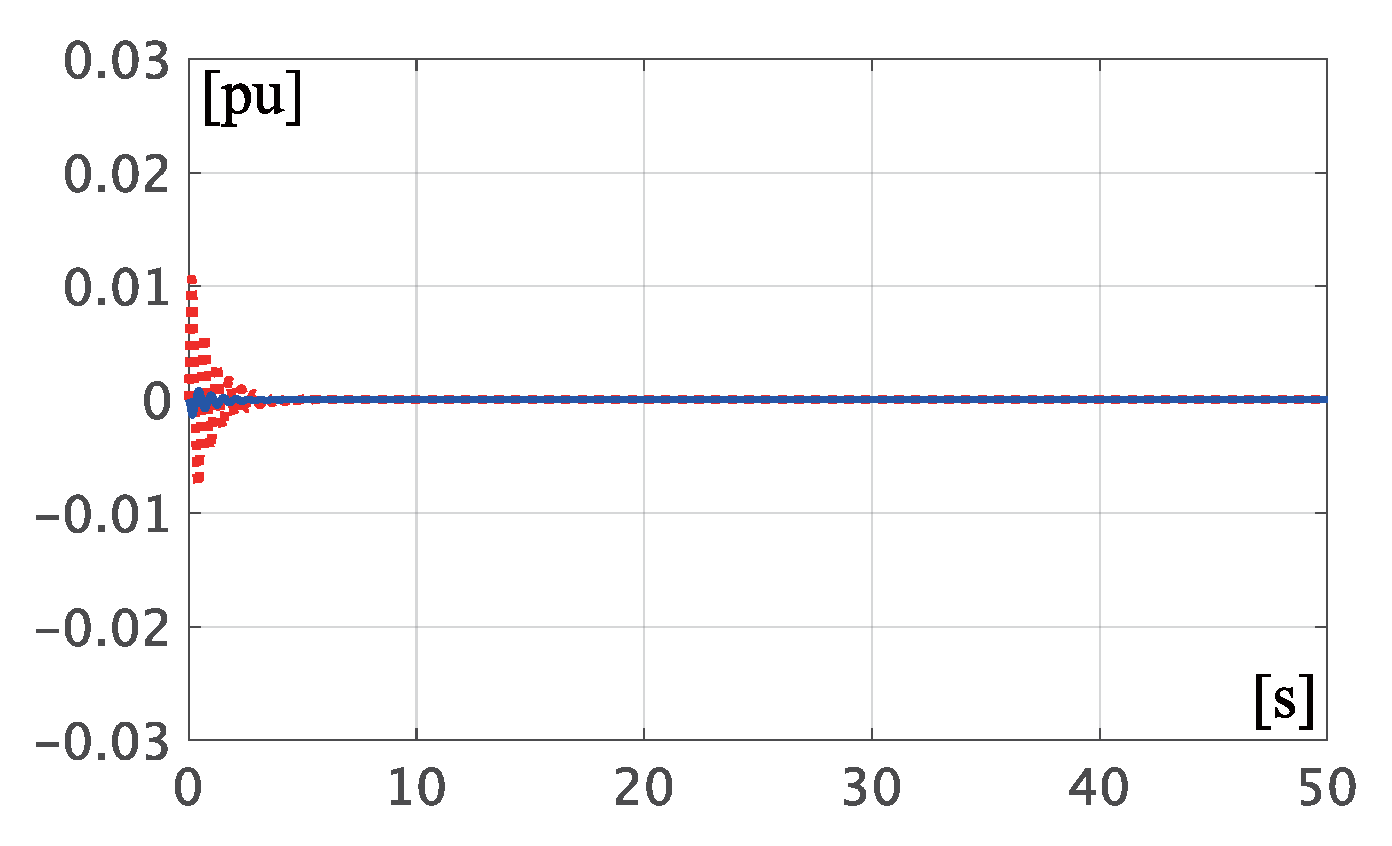
\includegraphics[width = 1.0\linewidth]{figs/wPSSsmall}
    \subcaption{ $\delta_1(0) - \delta_3(0) =-1$}
  \end{minipage}
  \begin{minipage}{0.49\linewidth}
    \centering
    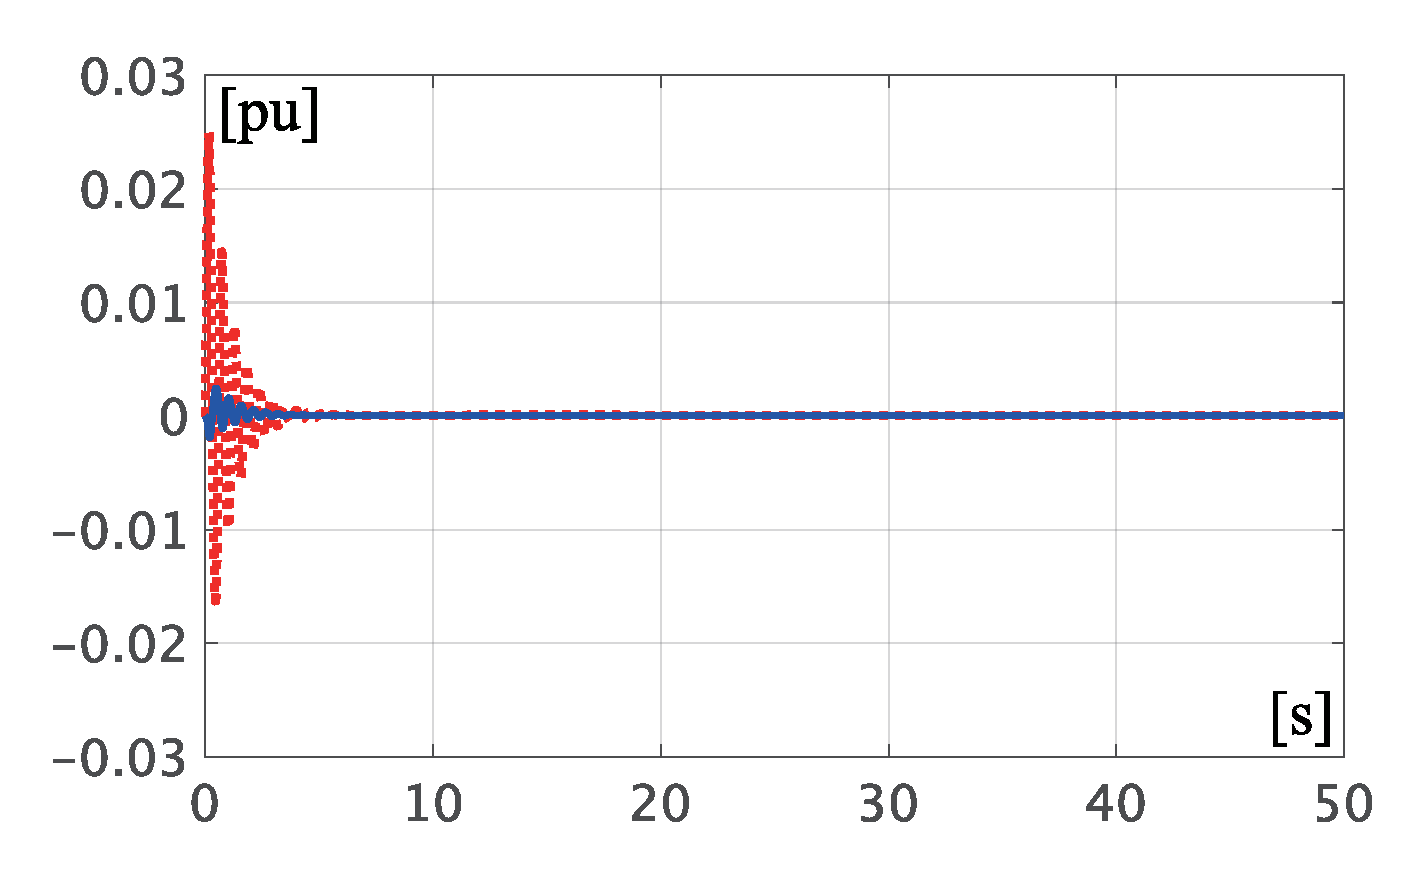
\includegraphics[width = 1.0\linewidth]{figs/wPSSlarge}
    \subcaption{ $\delta_1(0) - \delta_3(0) =-1.57$}
  \end{minipage}
  \medskip
  \caption{\textbf{Initial value response of angular frequency deviation}
  \\ \centering(There is a system stabilizer, and the line type is the same as \ref{fig: avrsmalld})}
  \label{fig:PSSomega}
  }
\medskip
\end{figure}

\section{PSS based on the retrofit control theory\advanced}\label{sec:retrofit}

\subsection{The electrical power system model used to design PSS\advanced}

\smallskip
\subsubsection{Characteristics of PSS based on the retrofit control theory}

In this Section, we explain the design method of PSS based on the retrofit control theory \cite{ishizaki2018retrofit,sadamoto2018retrofit,sasahara2019damping,ishizaki2019retrofit,ishizaki2021modularity}.
PSS designed with this method is able to stably maintain the steady power flow distribution of interest even when multiple generators are incorporated in parallel.
Specifically, each PSS is characterized as follows:
\begin{itemize}
\item Distributed design is possible with just a mathematical model of generators and AVR that incorporates it.
\item Distributed implementation is possible with just the local measurement signal of the voltage phasor and current phasor of generator buses.
\end{itemize}
Below, let us consider a situation where the IEEE ST1 Type AVR model of Equation \ref{eq:avrst1} is incorporated into the generator model of Equation \ref{eq:gendifavr}.
However, for a simpler explanation, we exclude the saturation of AVR.
If not only the cases with saturation but also other forms of AVR are incorporated, an existing PSS is incorporated, or more detailed generator models are used, the same discussion applies.

\smallskip
\subsubsection{Localized linear subsystem}

Let us consider expressing a localized subsystem with AVR connected to generators of interest as a linear system by improving the setting of interaction input:
\begin{align}\label{eq:desmodl}
G:\simode{
\dot{x} &= Ax + Bu + Lv \\
w &= \mathit{\Gamma} x \\
y &= Cx
}
\end{align}
where state $x$ is a vector with the state of the generator model $\delta$, $\Delta \omega$,$E$, and the state of the AVR model $V_{\rm tr}$ in that order.
Input $u$ expresses the output of PSS $V_{\rm pss}$, and input and output of interaction, $v$ and $w$, are defined as follows:
\begin{align}\label{eq:sigintvw}
v:=
\mat{
P_{\rm mech} - \tfrac{E |\bm{V} |}{ \Xt } \sfsin(\delta -  \angle \bm{V}) \\
k_{\rm ap} V_{\rm ref}^{\star} + 
\left(
\tfrac{ \Xs }{ \Xt }-1
\right)
|\bm{V}| \sfcos (\delta - \angle \bm{V} )\\
|\bm{V}|
}
,\qquad
w:=\mat{
\delta \\
\Delta \omega \\
E 
}
\end{align}
Please note that the interaction input $v$ of Equation \ref{eq:sigintvw} includes the nonlinear term of generators and variables of the bus bar voltage phasor.
With the definition of these signals, the system matrix of Equation \ref{eq:desmodl} is defined as:
\begin{align}\label{eq:matlocalm}
\spliteq{
A&:=\mat{
0 & \omega_0 & 0 & 0 \\
0 & -\tfrac{D}{M} & 0 & 0 \\
0 & 0 & -\tfrac{ \Xs }{ \taud \Xt } & -\tfrac{k_{\rm ap}}{ \taud } \\
0 & 0 & 0 & -\tfrac{1}{\tau_{\rm tr}}
}, \quad
B:=
\mat{
0 \\
0 \\
\tfrac{k_{\rm ap}}{ \taud } \\
0 
},\quad
C:= I \\
L &:=
\mat{
0 & 0 & 0 \\
\tfrac{1}{M} & 0 & 0 \\
0 & \tfrac{1}{ \taud } & 0 \\
0 & 0 & \tfrac{1}{\tau_{\rm tr} }
}, \quad
\mathit{\Gamma} :=
\mat{
1 & 0 & 0 & 0 \\
0 & 1 & 0 & 0 \\
0 & 0 & 1 & 0 
}
}
\end{align}
$G$ of Equation \ref{eq:desmodl} is called a \textbf{local linear subsystem}.
It is assumed that the parameters of the system matrix of Equation \ref{eq:matlocalm}, in other words, the model parameters of the local linear subsystem, are known and can be used to design and implement PSS.


\smallskip
\subsubsection{Environment and the approximate linear environment model}

Under the assumption that the output $y$ and input and output of interaction, $v$ and $w$, can be calculated, let us design a local controller that expresses PSS:
\[
K : (y,v,w)\mapsto u
\]
%ただし,式\ref{eq:desmodl}の局所線形サブシステム$G$では,出力$w$は出力$y$に包含されることに注意されたい。
Hereafter, we call this controller $K$ as a \textbf{retrofit controller}.
The word retrofit was derived from retroactive and refit, meaning performing partial expansions and renovations to an existing system.

For design and implementation of the retrofit controller, not only the model of the local linear subsystem $G$, but also a linear model that plays a role in the internal estimate of interaction input $v$ based on the information of interaction output $w$ is used.
Below, we called this estimate model the \textbf{approximate linear environment model}.

\begin{figure}[t]
\centering
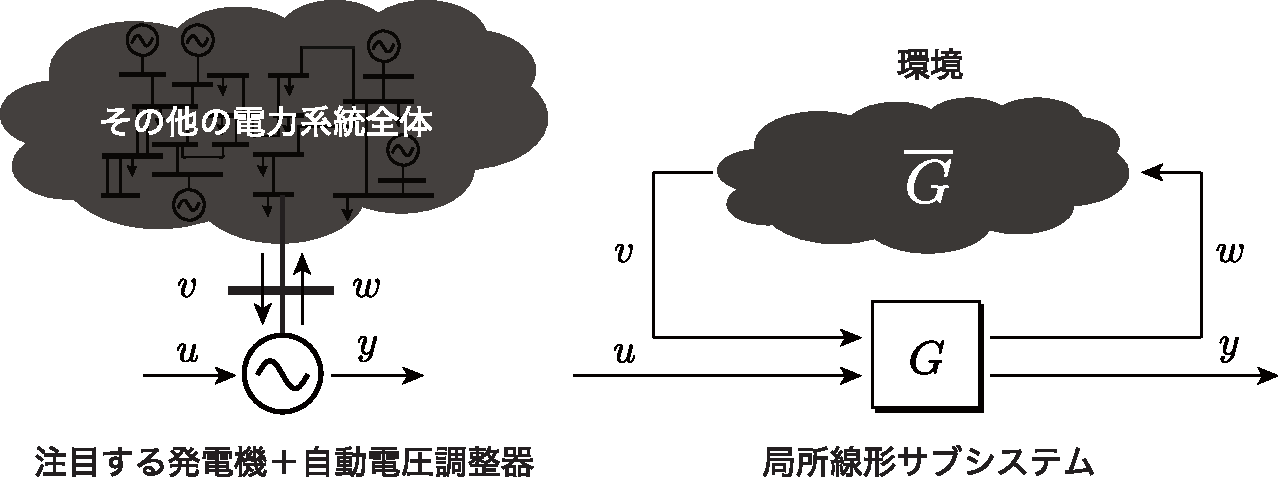
\includegraphics[width = .99\linewidth]{figs/retconsys2}
\medskip
\caption{\textbf{Coupling system of local linear subsystem and environment}}
\label{fig:retconsys}
\medskip
\end{figure}


In preparation for explaining the approximate linear environment model, we introduce a nonlinear subsystem called the \textbf{environment}.
The environment is a global subsystem that expresses “the entire system excluding the local linear subsystem”, which is a nonlinear system that uses the interaction output of the local linear subsystem $w$ as the input, and interaction input $v$ as the output.
Formally, we will present the dynamic relationship of the environment input and output as:
\[
\overline{G} : w\mapsto v
\]
Here, the feedback connection system of the local linear subsystem $G$ and the environment $\overline{G}$ expresses “the entire electrical power system from a viewpoint of the generators of interest” (\FIGref{fig:retconsys}).

Since the environment $\overline{G}$ includes multiple elements, such as power grids, loads, and other generators, it is not realistic to assume that the perfect nonlinear model of environment could be used to design and implement PSS for generators of interest.
Considering this fact, let us imagine a situation where “only the approximate linear environment model” is usable.
Before, for simplification, we consider expressing the approximate linear environment model with a static input-output relationship.
A dynamic approximate linear environment model can be used as well.
Please see \cite{ishizaki2019retrofit} for further details.

Specifically, when expressing the steady value of the interaction input-output under a steady power flow distribution of interest as $(v^{\star},w^{\star})$, the approximate linear environment model is parameterized as:
\begin{align}\label{eq:Gbapxst}
\overline{G}_{\rm apx}:
v_{\rm apx} = v^{\star} + \overline{\mathit{\Theta}} \left(w-w^{\star}\right)
%+ \overline{v}
\end{align}
Here, $\overline{\mathit{\Theta}}$ is a matrix that expresses the model parameters.
The approximate linear environment model $\overline{G}_{\rm apx}$ of Equation \ref{eq:Gbapxst} generates the value $v_{\rm apx}$ that estimates the steady values $(v^{\star},w^{\star})$ of impact of the interaction output $w$ on the interaction input $v$ by approximate linear prediction.
The electrical power system model used to design the retrofit controller is created through feedback connection of the parameters of this approximate linear environmental model $\overline{\mathit{\Theta}}$ and the model of the local linear subsystem $G$ (\FIGref{fig:explocalG}).
Specifically:
\begin{align}\label{eq:Gplus}
G^+: \simode{
\dot{\hat{\xi}} &=  \left( A+L \overline{\mathit{\Theta}} 
\mathit{\Gamma} \right) \hat{\xi} + B \hat{u} \\
\hat{y} & = C \hat{\xi}
}
\end{align}
%ただし,システム行列は
%\[
%A_+ :=
%A+L \overline{\mathit{\Theta}} 
%\mathit{\Gamma}
%,\qquad
%B_+ := B
%,\qquad
%C_+ := C
%\]
%である。
However, since $\hat{u}$ and $\hat{y}$ are virtual input and output signals to design the controller, we differentiated them from $u$ and $y$ with \^{ }.
Since $C$ is an identity matrix in Equation \ref{eq:matlocalm}, output $\hat{y}$ is equal to the internal state $\hat{\xi}$ of $G^+$.

\begin{figure}[t]
\centering
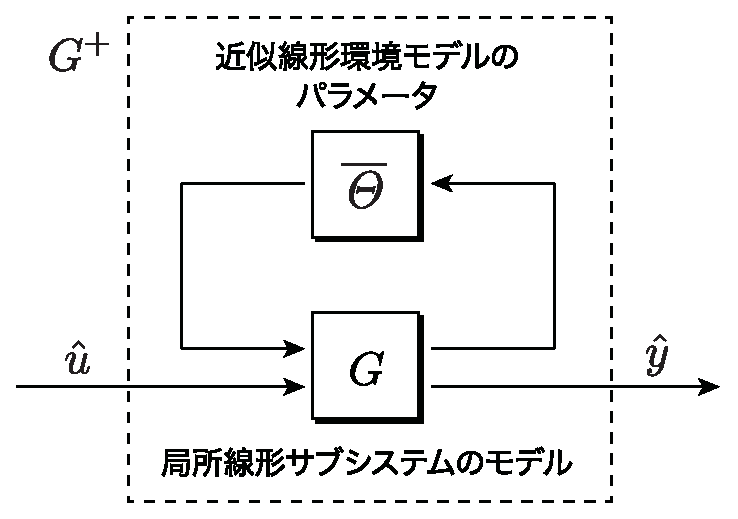
\includegraphics[width = .50\linewidth]{figs/explocalG2}
\medskip
\caption{\textbf{Model used for controller design}}
\label{fig:explocalG}
\medskip
\end{figure}

\subsection{PSS design based on the retrofit control theory\advanced}\label{sec:designret}

\smallskip
\subsubsection{Retrofit controller design method}

In this part, we assume that the approximate linear environment parameters $\overline{\mathit{\Theta}}$ of Equation \ref{eq:Gbapxst} are determined with an appropriate method and explain the design method for the retrofit controller.
The specific steps to create the approximate linear environment model are explained in the next part.

To design a retrofit controller that corresponds to PSS, the standard control system design method in control systems engineering can be used.
For example, let us apply the design method \cite[Section 5.3]{fairman1998linear} of \textbf{ linear-quadratic regulator (LQR)} to the controller design model $G^+$ of Equation \ref{eq:Gplus}.
With LQR, as a state feedback-style control algorithm to minimize the cost function related to the state and input:
\[
J(\hat{\xi},\hat{u}) :=\int_0^{\infty} \left(
\hat{\xi}^{\sf T}(t) Q \hat{\xi}(t)
+
\hat{u}^{\sf T}(t) R \hat{u}(t)
\right) dt
\]
we use the following:
\begin{align}\label{eq:locKhat}
\hat{u}=\underbrace{-R^{-1}B^{\sf T}P(\overline{\mathit{\Theta}}) }_{\hat{K}(\overline{\mathit{\Theta}}) }
\hat{\xi}
\end{align}
where, $Q$ is a positive semi-definite vector and $R$ is a positive definite vector.
The matrix $P(\overline{\mathit{\Theta}})$ is a positive definite solution that satisfies the \textbf{algebraic Riccati equation}.
\[
\left( A+L \overline{\mathit{\Theta}} 
\mathit{\Gamma} \right)^{\sf T} P +
P \left( A+L \overline{\mathit{\Theta}} 
\mathit{\Gamma} \right)
-PB R^{-1} B^{\sf T} P +Q = 0
\]
At this time, using the gain matrix $\hat{K}(\overline{\mathit{\Theta}})$ of Equation \ref{eq:locKhat}, the retrofit controller is built as follows:
\begin{align}\label{eq:retroK}
K: \simode{
\dot{\hat{x}} &=  A \hat{x} + L \left\{
v - \overline{\mathit{\Theta}} (w- \mathit{\Gamma} \hat{x}) 
\right\}\\
u &= \hat{K}(\overline{\mathit{\Theta}}) (y - C\hat{x})
}
\end{align}
PSS based on this retrofit control theory has the following characteristics with any matrix $\overline{\mathit{\Theta}}$ used:
\begin{itemize}
\item If the electrical power system is in a steady power flow distribution, input $u$ becomes 0.
\item Before and after implementation, the stability of the steady power flow distribution (equilibrium point) does not change.
\end{itemize}
The first item means that the retrofit controller does not change the steady state.
The second term means that the equilibrium point that was asymptotically stable before the implementation of the local controller does not change to an unstable equilibrium point because of the local controller.
With the retrofit control theory, it aims to “improve the stability” with robustness against disturbances and the size of the stable range as indicators while maintaining the asymptotic stability of the equilibrium point.
With this method, asymptotic stabilization of unstable equilibrium points is not possible.

Generally, as the prediction accuracy of interaction signals by the approximate linear environment model improves, the system stability improves greatly.
The control algorithm of Equation \ref{eq:locKhat} can be designed with other control system design methods as long as $G^+$ of Equation \ref{eq:Gplus} is stabilized.
$\hat{K}(\overline{\mathit{\Theta}})$ does not have to be static and can be used as a dynamic control algorithm \cite{ishizaki2019retrofit}.

\smallskip
\subsubsection{Method to build the approximate linear environment model}

One of the practical approaches to identify parameters $\overline{\mathit{\Theta}}$ of Equation \ref{eq:Gbapxst} is a method to estimate the relationship between signals $w$ and $v$ of Equation \ref{eq:sigintvw} with approximate linearization.
Specifically, partial differential of $v$ related to each element of $w$ is calculated as follows:
\begin{align}
\spliteq{
\frac{\partial v }{\partial \delta} &= 
\mat{
- \tfrac{E |\bm{V} |}{ \Xt } \sfcos(\delta -  \angle \bm{V})  \\
- \left( \tfrac{\Xs }{ \Xt }-1 \right)
|\bm{V}| \sfsin (\delta - \angle \bm{V} ) \\
0
}
, \qquad
\frac{\partial v }{\partial \Delta \omega} = \mat{0 \\0\\0} \\
\frac{\partial v }{\partial E} &= 
\mat{
- \tfrac{|\bm{V} |}{ \Xt } \sfsin(\delta -  \angle \bm{V}) \\
0\\
0
}
}
\end{align}
Therefore, if we assume that the internal state of the generators of interest and the voltage phasor of the generator buses are near steady power flow distribution, the following is obtained:
\begin{align}\label{eq:basenvm}
\overline{\mathit{\Theta}}^{\rm int} :=
\mat{
- \tfrac{E^{\star} |\bm{V}^{\star} |}{ \Xt } \sfcos(\delta^{\star} -  \angle \bm{V}^{\star}) &
0   & 
- \tfrac{|\bm{V}^{\star} |}{ \Xt } \sfsin(\delta^{\star} -  \angle \bm{V}^{\star})
\\
- \left( \tfrac{ \Xs }{ \Xt }-1 \right) 
|\bm{V}^{\star}| \sfsin (\delta^{\star} - \angle \bm{V}^{\star} ) 
& 0 
& 0 
\\
0 & 0 &0
}
\end{align}
where the steady value $(\delta^{\star},E^{\star})$ of the internal state of the generators and the steady value $(|\bm{V}^{\star}|,\angle \bm{V}^{\star})$ of the bus bar voltage phasor are the values from the same steady power flow distribution of $(v^{\star},w^{\star})$ in Equation \ref{eq:Gbapxst}.
With the matrix $\overline{\mathit{\Theta}}^{\rm int}$ of Equation ref{eq:basenvm}, “a local feedback structure of the internal state of generators on itself” can be modelled.
Since a regular electrical power system is operated near a steady power flow distribution, the steady value necessary to build the model can be identified based on measurement data.

Next, let us estimate the indirect impact of the signal $w$ on the signal $v$ through the automatic generation control.  The partial differential of $v$ related to the input $P_{\rm mech}$ of the automatic generation control is:
\[
\frac{\partial v}{\partial P_{\rm mech}}
=
\mat{
1\\0\\0
}
\]
If the broadcast-type PI controller of Equation (\ref{eq:agccon}) is incorporated as the automatic generation control, since the time integral of $\omega_0 \Delta \omega$ is equivalent to $\delta$:
\[
\frac{\partial P_{\rm mech}}{\partial \delta} = -  \frac{\alpha \beta k_{\rm I}}{\omega_0} 
,\qquad
\frac{\partial P_{\rm mech}}{\partial \Delta \omega}= - \alpha \beta k_{\rm P}
,\qquad
\frac{\partial P_{\rm mech}}{\partial E}= 0
\]
Thus, because of the chain rule of differentials, the impact of the signal $w$ on the signal $v$ through the broadcast-type PI controller can be modelled as:
\begin{align}
\overline{\mathit{\Theta}}^{\rm agc}:=
-  \alpha \beta \mat{
\tfrac{k_{\rm I}}{\omega_0} & k_{\rm P}  & 0\\
0 & 0 & 0\\
0 & 0 & 0
}
\end{align}
To obtain this parameter, the controller gain of the automatic generation control must be acquired with an appropriate method.

Similarly, let us estimate the indirect impact of the signal $w$ on the signal $v$ through the bus bar voltage phasor $\bm{V}$.
The partial differential of $v$ related to voltage phasor variables $(|\bm{V}|,\angle \bm{V})$ can be calculated as:
\begin{align}
\spliteq{
\frac{\partial v }{\partial |\bm{V}|} &= 
\mat{
-\tfrac{E }{ \Xt } \sfsin(\delta -  \angle \bm{V})  \\
\left( \tfrac{ \Xs }{ \Xt }-1 \right)
\sfcos (\delta - \angle \bm{V} ) \\
1
}
\\
\frac{\partial v }{\partial \angle \bm{V}} &= 
\mat{
\tfrac{E|\bm{V} |}{ \Xt } \sfcos(\delta -  \angle \bm{V}) \\
\left( \tfrac{ \Xs }{ \Xt }-1 \right)
|\bm{V}|\sfsin (\delta - \angle \bm{V} ) \\
0
}
}
\end{align}
Meanwhile, as analyzed in Section \ref{sec:allgen}, the bus bar voltage phasor
changes not only based on the internal state of the connected generator but also
dependent on the internal state of all the other generators. Specifically, when
the vectors of the internal state of all generators excluding the generator of
interest are expressed as $\overline{\delta}$, $\overline{E}$, the four partial
differentials
$\tfrac{\partial |\bm{V}| }{\partial \delta}$,
$\tfrac{\partial \angle \bm{V} }{\partial \delta}$,
$\tfrac{\partial |\bm{V}| }{\partial E}$,
$\tfrac{\partial \angle \bm{V} }{\partial E}$become a function that depends on the summary of the
internal state of all generators:
\[
z_{\mathds G}:=(\delta,\overline{\delta},E,\overline{E})
\]
It is not easy to analytically obtain these partial derivatives for a typical electrical power system model, but if the values:
\begin{align}\label{eq:thetaV}
\theta
:=
\mat{
\tfrac{\partial |\bm{V}| }{\partial \delta}(z_{\mathds G}^{\star}) &
0 &
\tfrac{\partial |\bm{V}| }{\partial E}(z_{\mathds G}^{\star}) \\
\tfrac{\partial \angle \bm{V} }{\partial \delta}(z_{\mathds G}^{\star}) &
0 &
\tfrac{\partial \angle \bm{V} }{\partial E}(z_{\mathds G}^{\star})
}
\end{align}
Could be determined using measurement data near a steady power flow distribution, the impact of the signal $w$ on the signal $v$ through the bus bar voltage phasor $\bm{V}$ can be modelled by:
\begin{align}\label{eq:ThetaV}
\overline{\mathit{\Theta}}^{\rm ext}:=
\mat{
-\tfrac{E^{\star} }{ \Xt } \sfsin(\delta^{\star} -  \angle \bm{V}^{\star}) 
 &
\tfrac{E^{\star}|\bm{V}^{\star} |}{ \Xt } \sfcos(\delta^{\star} -  \angle \bm{V}^{\star}) 
\\
\left( \tfrac{ \Xs }{ \Xt }-1 \right)
\sfcos (\delta^{\star} - \angle \bm{V}^{\star} )  
&
\left( \tfrac{ \Xs }{ \Xt }-1 \right)
|\bm{V}^{\star}|\sfsin (\delta^{\star} - \angle \bm{V}^{\star} )
\\
1 & 0
}
\hat{\theta}
\end{align}
$z_{\mathds G}^{\star}$ of Equation \ref{eq:thetaV} expresses the steady value of $z_{\mathds G}$, and the 0 element on the second column corresponds to $\tfrac{\partial |\bm{V}| }{\partial \Delta \omega}$,$\tfrac{\partial \angle \bm{V} }{\partial \Delta \omega}$.
$\hat{\theta}$ of Equation \ref{eq:ThetaV} expresses the identified values of $\theta$.
$\overline{\mathit{\Theta}}^{\rm ext}$ of Equation \ref{eq:ThetaV} models “a global feedback structure the internal state of generators provides to itself.
This is in contrast to $\overline{\mathit{\Theta}}^{\rm int}$ of Equation \ref{eq:basenvm} that models the local feedback structure.

Since the electrical power system must be always in a stable operation, parameters $\hat{\theta}$ of Equation \ref{eq:ThetaV} must be determined using the data measured in operation.
In control systems engineering, determination of the subsystem in an operating feedback system is called \textbf{closed-loop identification}.
Since closed-loop identification cannot freely excite the input of the identification target, it is often more difficult than identification when excitation of input is possible.

If using the above estimates by approximate linearization simultaneously, model parameters of Equation \ref{eq:Gbapxst} are structured as follows:
\begin{align}\label{eq:Thetasum}
\overline{\mathit{\Theta}}=
\overline{\mathit{\Theta}}^{\rm int}+
\overline{\mathit{\Theta}}^{\rm agc}+
\overline{\mathit{\Theta}}^{\rm ext}
\end{align}
As discussed in the previous part, the retrofit controller of Equation \ref{eq:retroK} does not change the stability of the steady power flow distribution for any matrix $\overline{\mathit{\Theta}}$.
In contrast, to maintain the prediction accuracy by the approximate linear environment model, $\overline{\mathit{\Theta}}$ should be updated at a frequency appropriate for the changes in the power flow distribution.

\begin{figure}[t]
%  \centering
%  {
%  \begin{minipage}{0.49\linewidth}
%    \centering
%    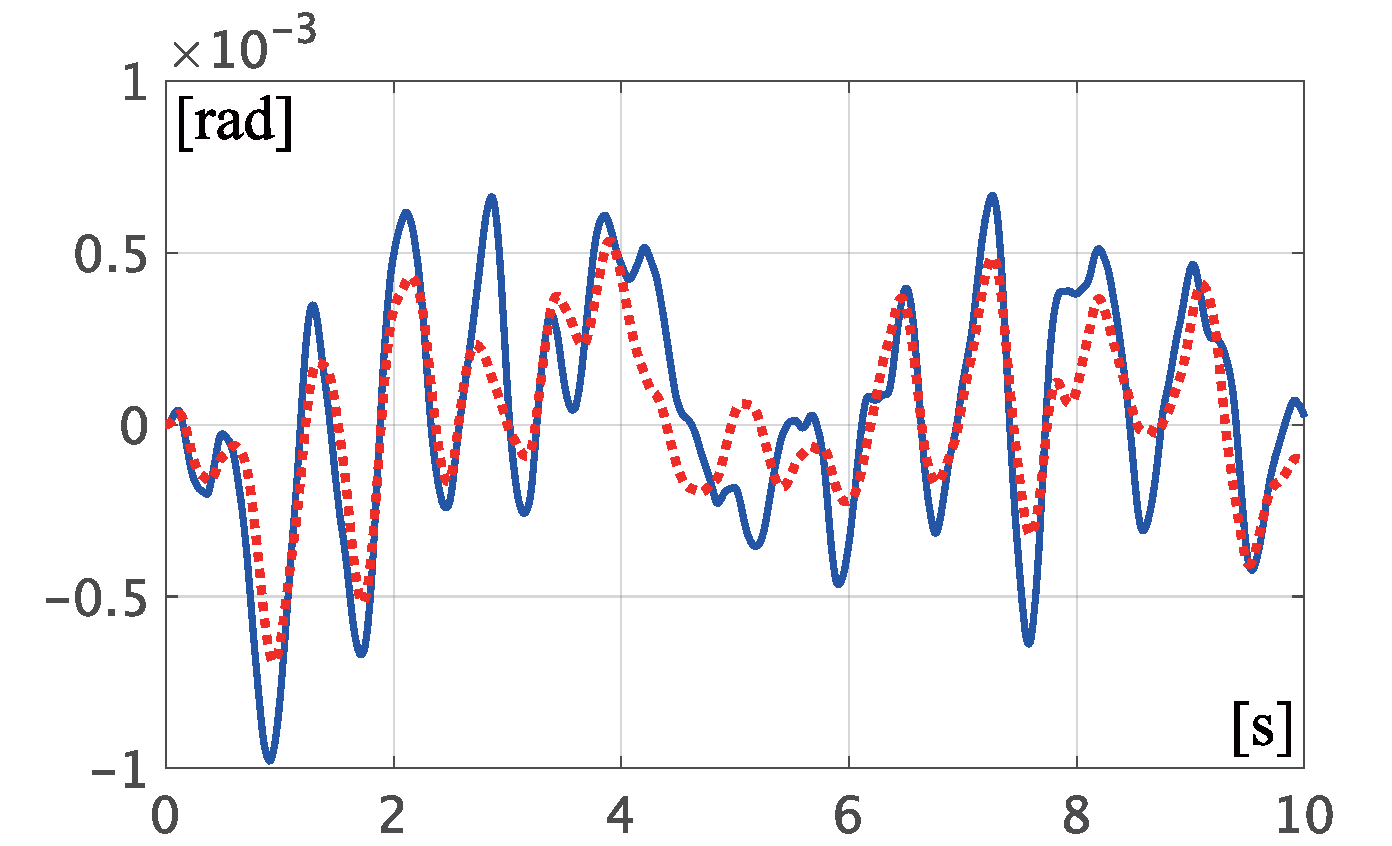
\includegraphics[width = 1.0\linewidth]{figs/timedeltamodel}
%    \subcaption{ $\delta_1$の時系列データ}
%     \medskip
%  \end{minipage}
%  \begin{minipage}{0.49\linewidth}
%    \centering
%    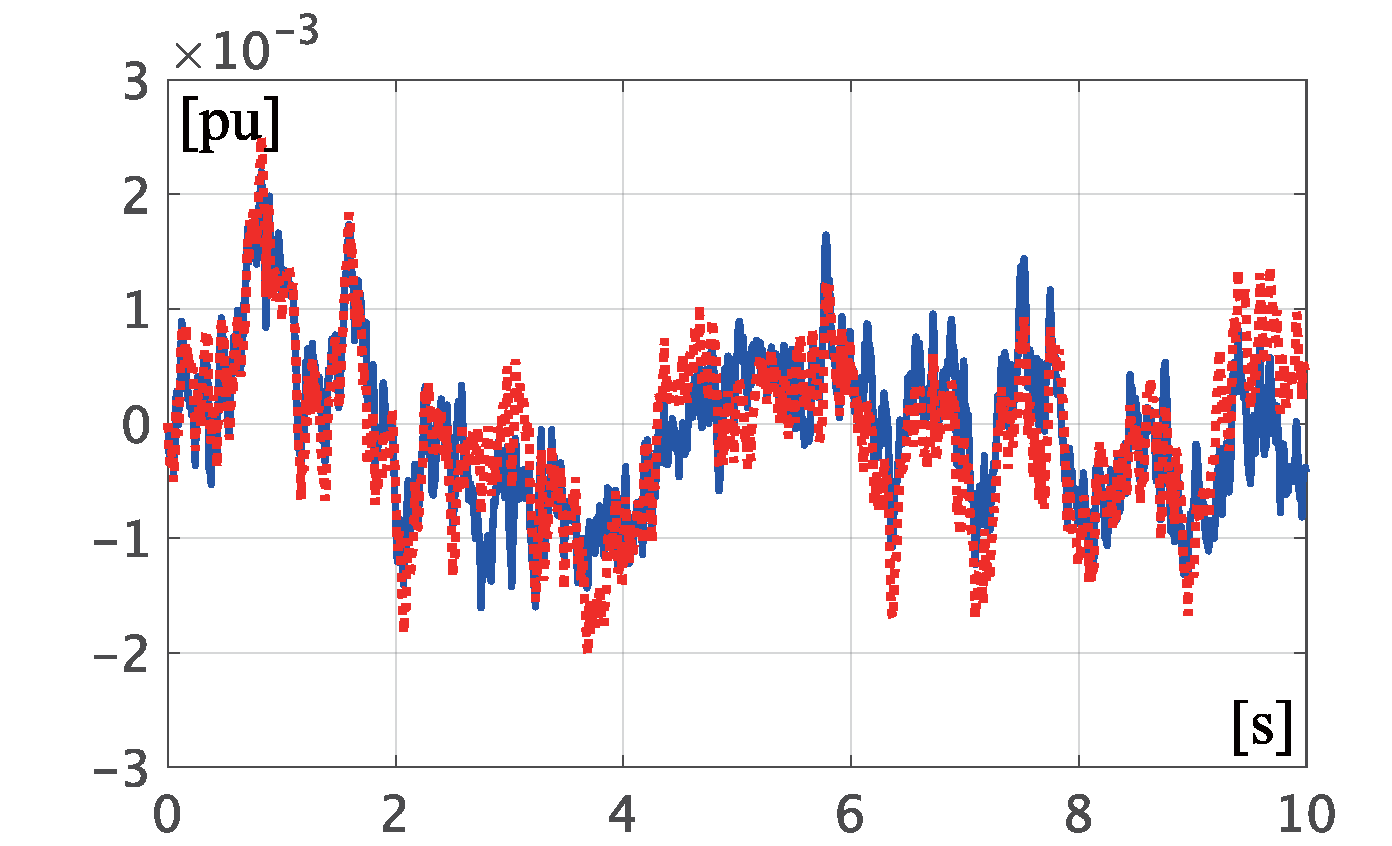
\includegraphics[width = 1.0\linewidth]{figs/timeEmodel}
%    \subcaption{ $E_1$の時系列データ}
%     \medskip
%  \end{minipage}
%    }
  \centering
  {
  \begin{minipage}{0.49\linewidth}
    \centering
    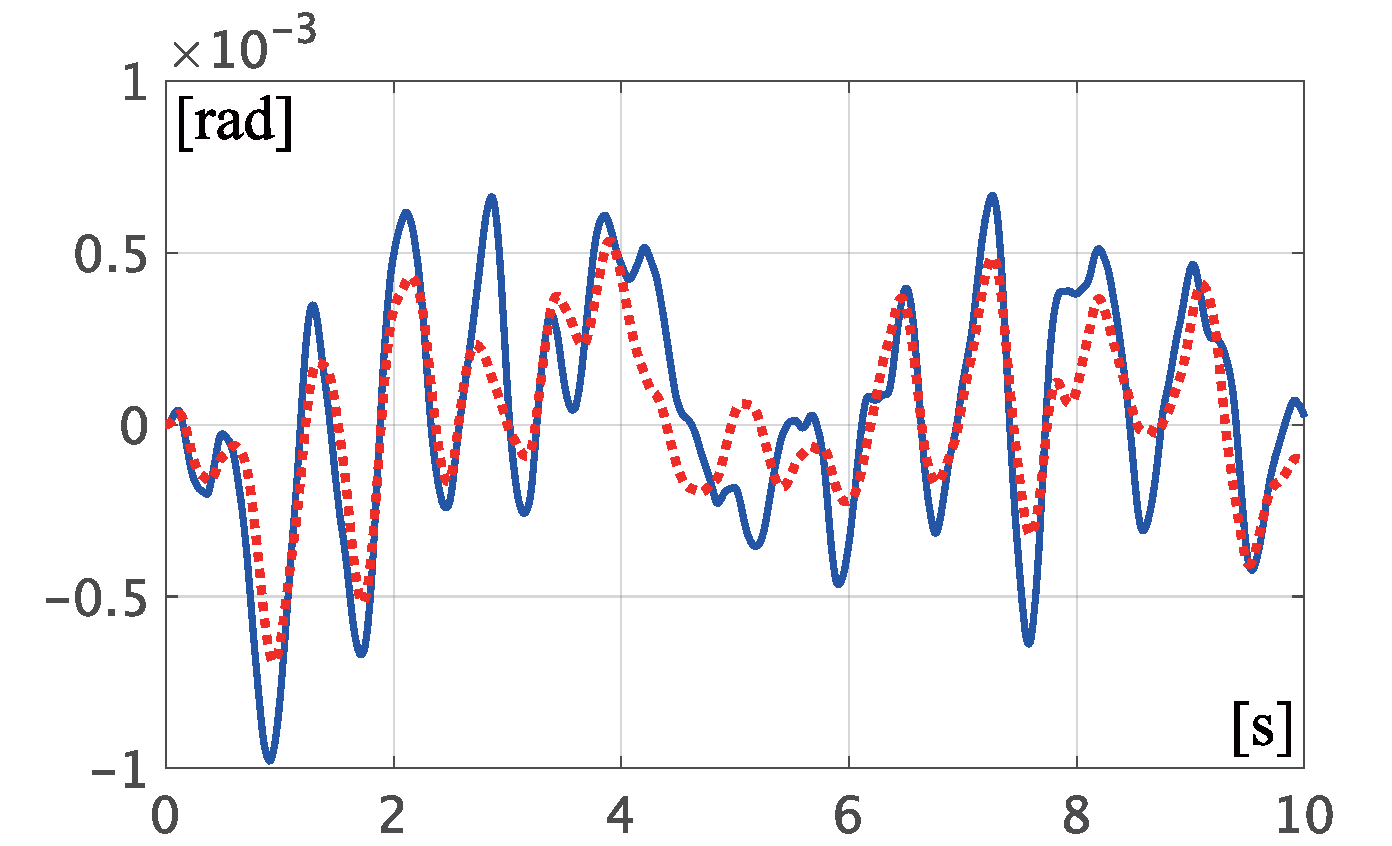
\includegraphics[width = 1.0\linewidth]{figs/timedeltamodel}
    \subcaption{Time series data of $\delta_3$ and $\hat{\delta}_3$}
     \medskip
  \end{minipage}
  \begin{minipage}{0.49\linewidth}
    \centering
    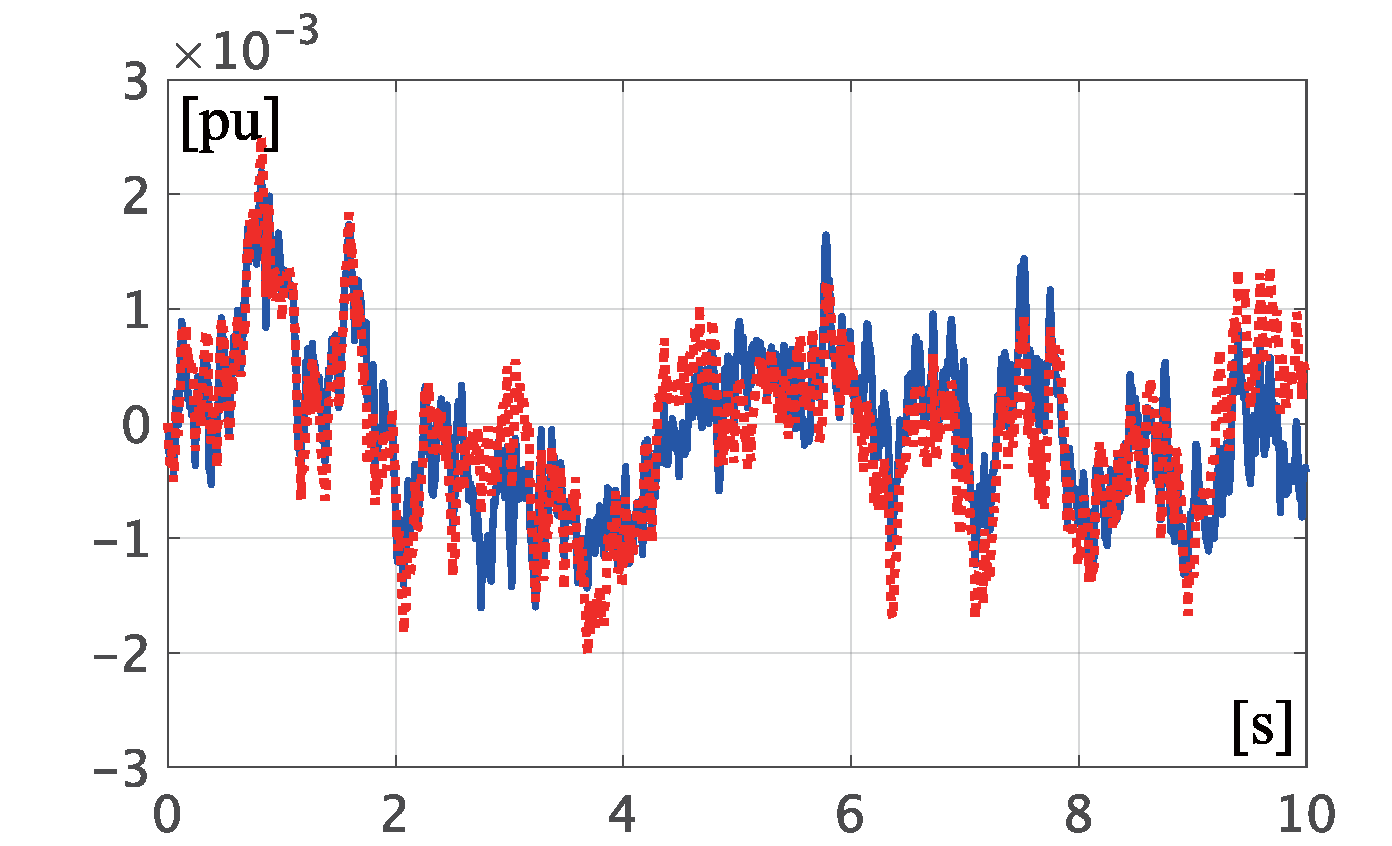
\includegraphics[width = 1.0\linewidth]{figs/timeEmodel}
    \subcaption{Time series data of $E_3$ and $\hat{E}_3$}
     \medskip
  \end{minipage}
    }
\caption{\textbf{Time response to random excitation input}
 \\ \centering(Blue solid line: $\delta_3, E_3$, Red dashed line: $\hat{\delta}_3,\hat{E}_3$)
 }
  \label{fig:timeVmodel}
\medskip
\end{figure}


\begin{figure}[t!]
  \centering
  {
  \begin{minipage}{0.49\linewidth}
    \centering
    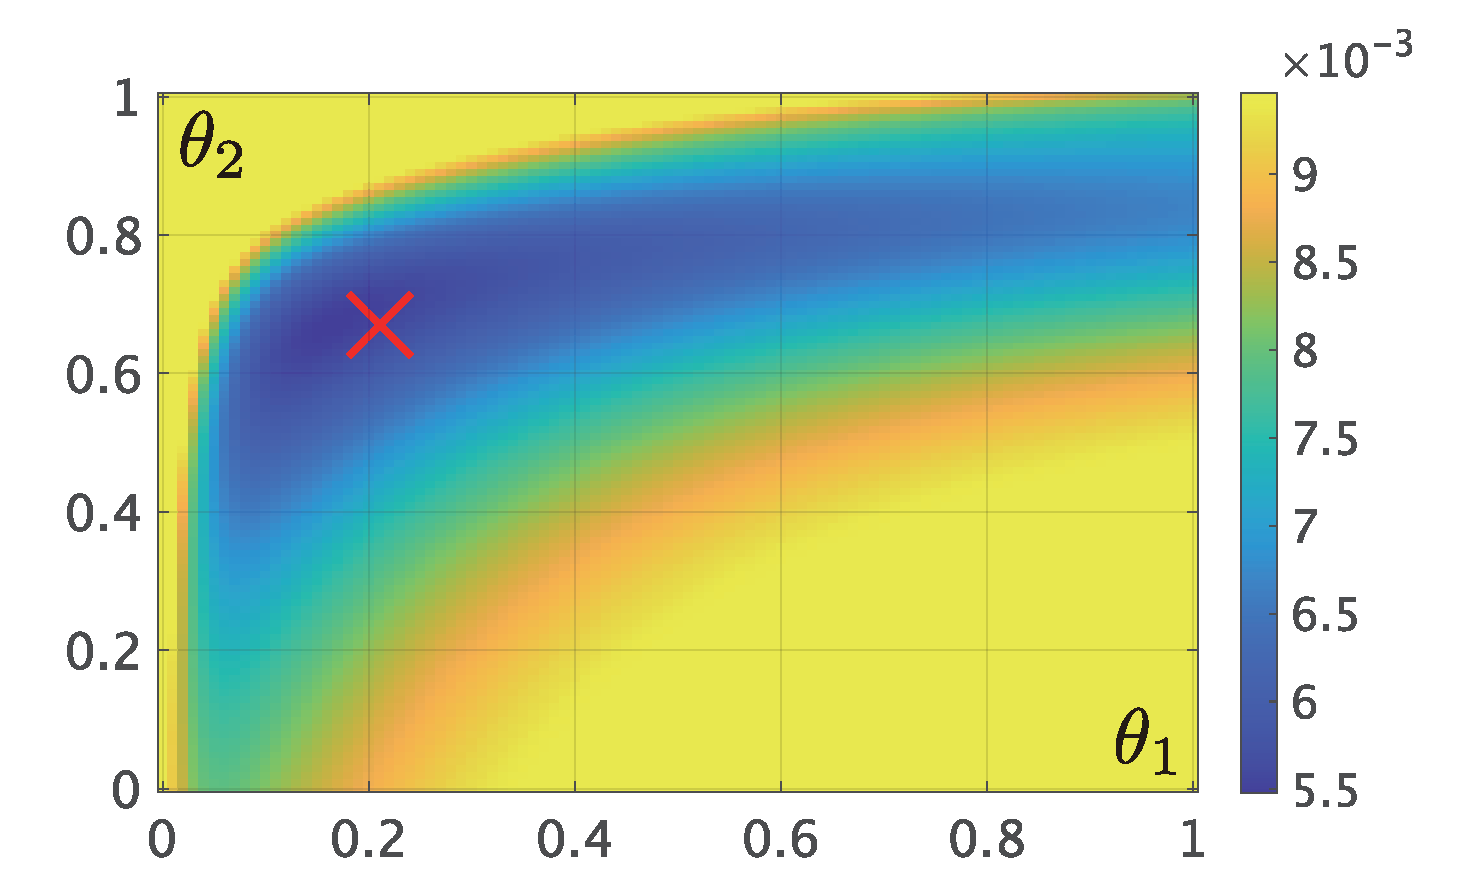
\includegraphics[width = 1\linewidth]{figs/heatdelta}
    \subcaption{ $Q(\delta_3,\hat{\delta}_3)$ }
    \medskip
  \end{minipage}
  \begin{minipage}{0.49\linewidth}
    \centering
    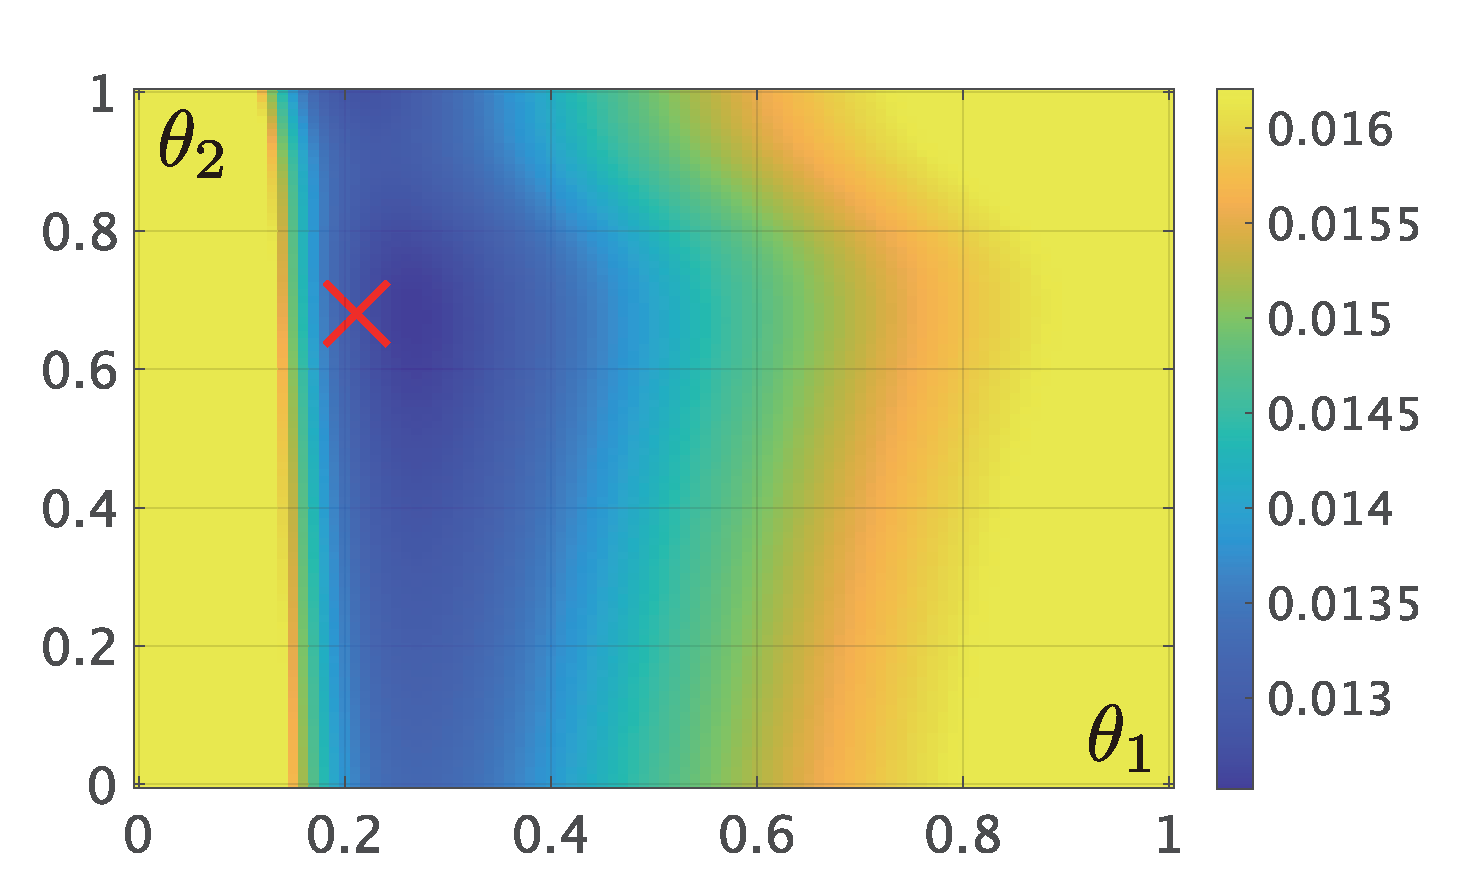
\includegraphics[width = 1\linewidth]{figs/heatE}
    \subcaption{ $Q(E_3,\hat{E}_3)$ }
    \medskip
  \end{minipage}
}
%  \centering
%  {
%  \begin{minipage}{0.49\linewidth}
%      \centering
%    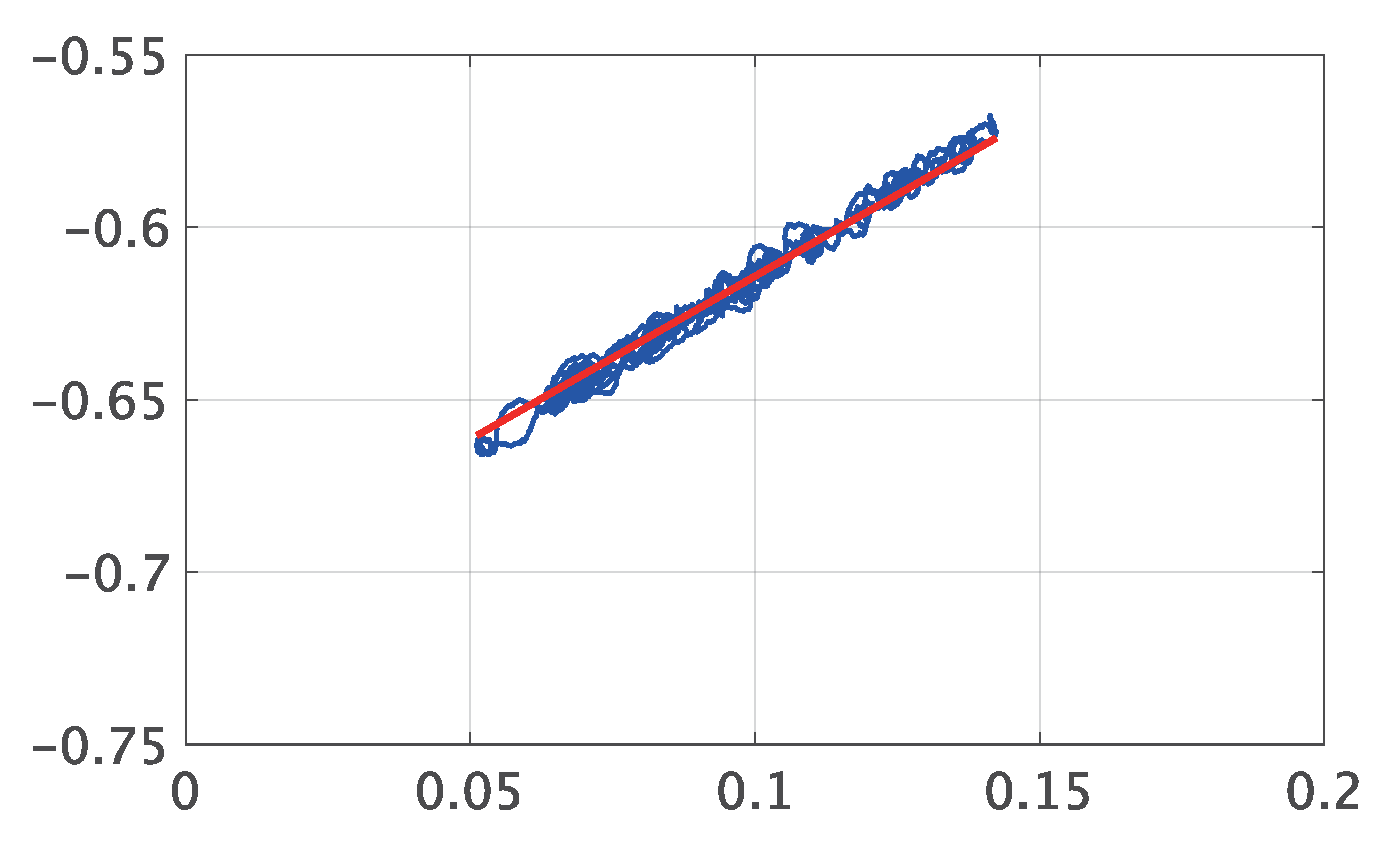
\includegraphics[width = 1\linewidth]{figs/angVdelta}
%    \subcaption{ $\bigl(\delta_1(\tfrac{k}{100}),\angle \bm{V}_1(\tfrac{k}{100}) \bigr)$ }
%    \medskip
%  \end{minipage}
%  \begin{minipage}{0.49\linewidth}
%    \centering
%    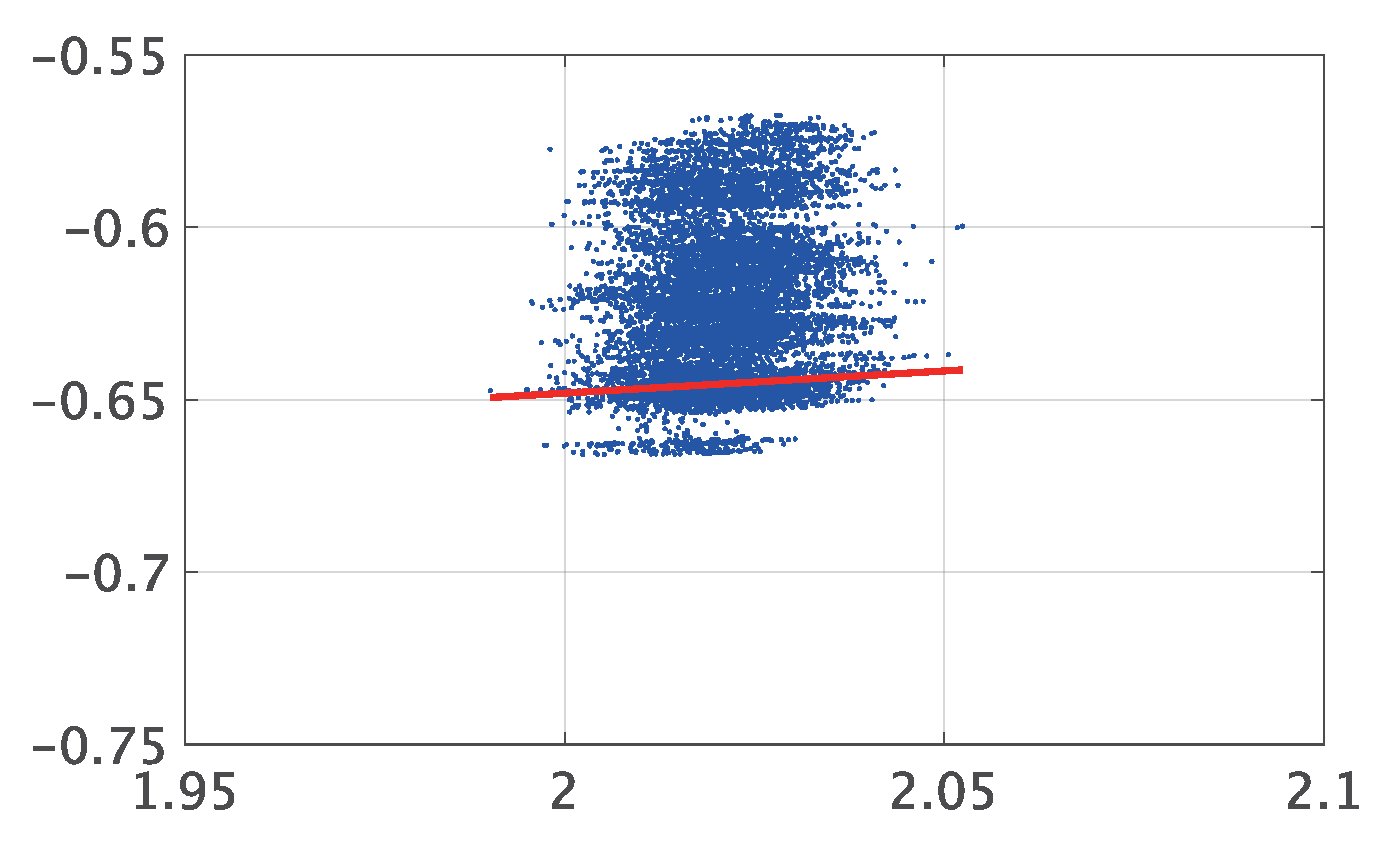
\includegraphics[width = 1\linewidth]{figs/angVE}
%    \subcaption{ $\bigl(E_1(\tfrac{k}{100}), \angle \bm{V}_1(\tfrac{k}{100}) \bigr)$ }
%    \medskip
%  \end{minipage}
%}
% \medskip
 \caption{\textbf{Approximation error of internal state with respect to identification parameter}}
 \label{fig:datamodeling}
\medskip
\end{figure}


\begin{例}[Identification of the approximate linear environment model based on measurement data]\label{ex:modelingV}
Similar to Example \ref{ex:avreffect}, let us consider the same AVR incorporated in generator 1 and generator 3 for the electrical power system model consisting of three bus bars.
Here, the broadcast-type PI controller of Equation (\ref{eq:agccon}), for which parameters of \ref{table:agcpara}(b) are set, is incorporated as the automatic generation control.
The steady power flow distribution corresponds to the power flow calculation result of \ref{table:pflow2}.

Below, we focus on generator 3, and identify the partial differential values, the element of $\theta_3$ of Equation \ref{eq:thetaV}, from measurement data. However, since the size of $\tfrac{\partial |\bm{V}_3|}{\partial \delta_3}(z_{\mathds G}^{\star})$ and $\tfrac{\partial \angle \bm{V}_3}{\partial E_3}(z_{\mathds G}^{\star})$ is relatively small, only two values of:
\[
\theta_1:=
\frac{\partial | \bm{V}_3|}{\partial E_3}(z_{\mathds G}^{\star})
,\qquad
\theta_2:=
\frac{\partial \angle \bm{V}_3}{\partial \delta_3}(z_{\mathds G}^{\star})
\]
are identified from the data. At this time, $\overline{\mathit{\Theta}}^{\rm ext}_3$ of Equation \ref{eq:ThetaV} is parametrized as:
\begin{align}\label{eq:Thext1para}
\overline{\mathit{\Theta}}^{\rm ext}_3=
\mat{
\tfrac{E_3^{\star}|\bm{V}_3^{\star} |}{ \Xt_3 } \Delta^{\sf cos}_3 \theta_2
& 
0
&
- \tfrac{ E_3^{\star} }{ \Xt_3 } \Delta^{\sf sin}_3 \theta_1
\\
\left( \tfrac{ \Xs_3 }{ \Xt_3 }-1 \right)
|\bm{V}_3^{\star}| \Delta^{\sf sin}_3 \theta_2
&
0
&
\left( \tfrac{ \Xs_3 }{ \Xt_3 }-1 \right)
 \Delta^{\sf cos}_3 \theta_1
\\
0 & 0 & \theta_1
}
\end{align}
where $\Delta^{\sf sin}_3$ and $\Delta^{\sf cos}_3$ are constants defined by:
\[
\Delta^{\sf sin}_3 := \sfsin(\delta_3^{\star} -  \angle \bm{V}_3^{\star}) ,\qquad
\Delta^{\sf cos}_3 := \sfcos (\delta_3^{\star} - \angle \bm{V}_3^{\star} )
\]

The optimization of parameters $(\theta_1,\theta_2)$ is performed with the following steps.
The time series data of $(\delta_3,E_3)$ obtained when the input of AVR $V_{{\rm pss}3}$ is randomly excited is acquired from the electrical power system.
In addition, for generator 3, a controller design model $G_{3}^+$ of Equation \ref{eq:Gplus} is built as a feedback system of parameters $\overline{\mathit{\Theta}}_3$ of the local linear subsystem $G_3$ of Equation \ref{eq:desmodl} and the approximate linear environment model.
$\overline{\mathit{\Theta}}_3$ is defined by Equation \ref{eq:Thetasum}.
At this time, as the first and the third elements of $\hat{y}_3$, when signals are added to the excitation of $V_{{\rm pss}3}$ as the input $\hat{u}_3$ of Equation \ref{eq:Gplus}, time series data of $(\hat{\delta}_3,\hat{E}_3)$ is obtained.
Parameters $(\theta_1,\theta_2)$ are optimized so that $\hat{\delta}_3(t)$ and $\hat{E}_3(t)$ become good approximations of $\delta_3(t)$ and $E_3(t)$ for all the time $t$ in the interval where the data was obtained.

%\[
%\delta_3(t) \simeq \hat{\delta}_3(t)
%,\qquad
%E_3(t) \simeq \hat{E}_3(t)
%\]

The blue line in \FIGref{fig:timeVmodel} shows the time series data of $(\delta_3,E_3)$ when $V_{{\rm pss}3}$ is randomly excited between 0 [s] to 10 [s].
The deviation against the steady value $(\delta_3^{\star},E_3^{\star})$ is being shown.
The result of a comprehensive search for the optimal parameters for this data $(\theta_1,\theta_2)$ over an even interval of 0.01 is shown in \FIGref{fig:datamodeling}.
The horizontal and vertical axes show the set values of $\theta_1$ and $\theta_2$, respectively, where the colors of the range of (a) and (b) show the errors $Q(\delta_3,\hat{\delta}_3)$,$Q(E_3,\hat{E}_3)$.
However, the following:
\[
Q(x,\hat{x}):=
\sum_{k=1}^{1000}
\left\|
x\left(
\tfrac{k}{100}
\right)
-
\hat{x}\left(
\tfrac{k}{100}
\right)
\right\|^2
\]
is a function that evaluates the error of 1,000 discrete time signals where continuous time signals $x(t)$,$\hat{x}(t)$ of $t\in [0,10]$ were sampled over a period of 0.01 [s].
Based on this result, we set the parameter values to $(0.215,0.675)$.
These parameter values correspond to "$\times$" of \FIGref{fig:datamodeling}.
The time series data of $(\hat{\delta}_3,\hat{E}_3)$ corresponding to this parameter setting is shown with the broken red line in \FIGref{fig:timeVmodel}.
With the obtained approximate linear environment model, we can see that the behavior of the internal state of generator 3 is captured.
\end{例}


In Example \ref{ex:modelingV}, the parameters of the approximate linear environment model are identified as the index of the precision by which the internal state of the generators is approximated.
The effect of the retrofit control based on this identification method is presented in Chapter \ref{chap:largesim}.

\newpage
%\printindex
%
%
\end{document}